% ******************************* PhD Thesis Template **************************
% Please have a look at the README.md file for info on how to use the template

\documentclass[a4paper,12pt,times,authoryear,print,index]{PhDThesisPSnPDF}

% ******************************************************************************
% ******************************* Class Options ********************************
% *********************** See README for more details **************************
% ******************************************************************************

% `a4paper'(The University of Cambridge PhD thesis guidelines recommends a page
% size a4 - default option) or `a5paper': A5 Paper size is also allowed as per
% the Cambridge University Engineering Deparment guidelines for PhD thesis
%
% `11pt' or `12pt'(default): Font Size 10pt is NOT recommended by the University
% guidelines
%
% `oneside' or `twoside'(default): Printing double side (twoside) or single
% side.
%
% `print': Use `print' for print version with appropriate margins and page
% layout. Leaving the options field blank will activate Online version.
%
% `index': For index at the end of the thesis
%
% `draftclassic': For draft mode without loading any images (same as draft in book)
%
% `draft': Special draft mode with line numbers, images, and water mark with
% timestamp and custom text. Position of the text can also be modified.
%
% `abstract': To generate only the title page and abstract page with
% dissertation title and name, to submit to the Student Registry
%
% `chapter`: This option enables only the specified chapter and it's references
%  Useful for review and corrections.
%
% ************************* Custom Page Margins ********************************
%
% `custommargin`: Use `custommargin' in options to activate custom page margins,
% which can be defined in the preamble.tex. Custom margin will override
% print/online margin setup.
%
% *********************** Choosing the Fonts in Class Options ******************
%
% `times' : Times font with math support. (The Cambridge University guidelines
% recommend using times)
%
% `fourier': Utopia Font with Fourier Math font (Font has to be installed)
%            It's a free font.
%
% `customfont': Use `customfont' option in the document class and load the
% package in the preamble.tex
%
% default or leave empty: `Latin Modern' font will be loaded.
%
% ********************** Choosing the Bibliography style ***********************
%
% `authoryear': For author-year citation eg., Krishna (2013)
%
% `numbered': (Default Option) For numbered and sorted citation e.g., [1,5,2]
%
% `custombib': Define your own bibliography style in the `preamble.tex' file.
%              `\RequirePackage[square, sort, numbers, authoryear]{natbib}'.
%              This can be also used to load biblatex instead of natbib
%              (See Preamble)
%
% **************************** Choosing the Page Style *************************
%
% `default (leave empty)': For Page Numbers in Header (Left Even, Right Odd) and
% Chapter Name in Header (Right Even) and Section Name (Left Odd). Blank Footer.
%
% `PageStyleI': Chapter Name next & Page Number on Even Side (Left Even).
% Section Name & Page Number in Header on Odd Side (Right Odd). Footer is empty.
%
% `PageStyleII': Chapter Name on Even Side (Left Even) in Header. Section Number
% and Section Name in Header on Odd Side (Right Odd). Page numbering in footer

% Uncomment to change page style
%\pagestyle{PageStyleII}

% ********************************** Preamble **********************************
% Preamble: Contains packages and user-defined commands and settings
% ******************************************************************************
% ****************************** Custom Margin *********************************

% Add `custommargin' in the document class options to use this section
% Set {innerside margin / outerside margin / topmargin / bottom margin}  and
% other page dimensions
\ifsetCustomMargin
  \RequirePackage[left=37mm,right=30mm,top=35mm,bottom=30mm]{geometry}
  \setFancyHdr % To apply fancy header after geometry package is loaded
\fi

% Add spaces between paragraphs
%\setlength{\parskip}{0.5em}
% Ragged bottom avoids extra whitespaces between paragraphs
\raggedbottom
% To remove the excess top spacing for enumeration, list and description
%\usepackage{enumitem}
%\setlist[enumerate,itemize,description]{topsep=0em}

% *****************************************************************************
% ******************* Fonts (like different typewriter fonts etc.)*************

% Add `customfont' in the document class option to use this section

\ifsetCustomFont
  % Set your custom font here and use `customfont' in options. Leave empty to
  % load computer modern font (default LaTeX font).
  %\RequirePackage{helvet}

  % For use with XeLaTeX
  %  \setmainfont[
  %    Path              = ./libertine/opentype/,
  %    Extension         = .otf,
  %    UprightFont = LinLibertine_R,
  %    BoldFont = LinLibertine_RZ, % Linux Libertine O Regular Semibold
  %    ItalicFont = LinLibertine_RI,
  %    BoldItalicFont = LinLibertine_RZI, % Linux Libertine O Regular Semibold Italic
  %  ]
  %  {libertine}
  %  % load font from system font
  %  \newfontfamily\libertinesystemfont{Linux Libertine O}
\fi

% *****************************************************************************
% **************************** Custom Packages ********************************

% ************************* Algorithms and Pseudocode **************************

%\usepackage{algpseudocode}


% ********************Captions and Hyperreferencing / URL **********************

% Captions: This makes captions of figures use a boldfaced small font.
%\RequirePackage[small,bf]{caption}

\RequirePackage[labelsep=space,tableposition=top]{caption}
\renewcommand{\figurename}{Fig.} %to support older versions of captions.sty


% *************************** Graphics and figures *****************************

%\usepackage{rotating}
%\usepackage{wrapfig}

% Uncomment the following two lines to force Latex to place the figure.
% Use [H] when including graphics. Note 'H' instead of 'h'
%\usepackage{float}
%\restylefloat{figure}

% Subcaption package is also available in the sty folder you can use that by
% uncommenting the following line
% This is for people stuck with older versions of texlive
%\usepackage{sty/caption/subcaption}
\usepackage{subcaption}

% ********************************** Tables ************************************
\usepackage{booktabs} % For professional looking tables
\usepackage{multirow}

%\usepackage{multicol}
%\usepackage{longtable}
%\usepackage{tabularx}


% *********************************** SI Units *********************************
%\usepackage{siunitx} % use this package module for SI units


% ******************************* Line Spacing *********************************

% Choose linespacing as appropriate. Default is one-half line spacing as per the
% University guidelines

% \doublespacing
% \onehalfspacing
% \singlespacing


% ************************ Formatting / Footnote *******************************

% Don't break enumeration (etc.) across pages in an ugly manner (default 10000)
%\clubpenalty=500
%\widowpenalty=500

%\usepackage[perpage]{footmisc} %Range of footnote options


% *****************************************************************************
% *************************** Bibliography  and References ********************

%\usepackage{cleveref} %Referencing without need to explicitly state fig /table

% Add `custombib' in the document class option to use this section
\ifuseCustomBib
   \RequirePackage[square, sort, numbers, authoryear]{natbib} % CustomBib

% If you would like to use biblatex for your reference management, as opposed to the default `natbibpackage` pass the option `custombib` in the document class. Comment out the previous line to make sure you don't load the natbib package. Uncomment the following lines and specify the location of references.bib file

%\RequirePackage[backend=biber, style=numeric-comp, citestyle=numeric, sorting=nty, natbib=true]{biblatex}
%\addbibresource{References/references} %Location of references.bib only for biblatex, Do not omit the .bib extension from the filename.

\fi

% changes the default name `Bibliography` -> `References'
\renewcommand{\bibname}{References}


% ******************************************************************************
% ************************* User Defined Commands ******************************
% ******************************************************************************

% *********** To change the name of Table of Contents / LOF and LOT ************

%\renewcommand{\contentsname}{My Table of Contents}
%\renewcommand{\listfigurename}{My List of Figures}
%\renewcommand{\listtablename}{My List of Tables}


% ********************** TOC depth and numbering depth *************************

\setcounter{secnumdepth}{2}
\setcounter{tocdepth}{2}


% ******************************* Nomenclature *********************************

% To change the name of the Nomenclature section, uncomment the following line

%\renewcommand{\nomname}{Symbols}


% ********************************* Appendix ***********************************

% The default value of both \appendixtocname and \appendixpagename is `Appendices'. These names can all be changed via:

%\renewcommand{\appendixtocname}{List of appendices}
%\renewcommand{\appendixname}{Appndx}

% *********************** Configure Draft Mode **********************************

% Uncomment to disable figures in `draft'
%\setkeys{Gin}{draft=true}  % set draft to false to enable figures in `draft'

% These options are active only during the draft mode
% Default text is "Draft"
%\SetDraftText{DRAFT}

% Default Watermark location is top. Location (top/bottom)
%\SetDraftWMPosition{bottom}

% Draft Version - default is v1.0
%\SetDraftVersion{v1.1}

% Draft Text grayscale value (should be between 0-black and 1-white)
% Default value is 0.75
%\SetDraftGrayScale{0.8}

% ******************* Better enumeration my MB*************
\usepackage{enumitem}

\usepackage{amsmath}
%\usepackage{amssymb}
\usepackage{bm} % bold maths symbols
\usepackage{graphicx}
\usepackage{float}
\usepackage{hyperref}
\usepackage{algorithm}
\usepackage{algpseudocode}
\usepackage{framed}

% ==============================================================================
% Maths commands
% ==============================================================================


\renewcommand{\vec}[1]{\mathbf{#1}}
\renewcommand{\d}{\,\text{d}}


\newcommand{\A}{\mathcal{A}}
\newcommand{\E}{\mathcal{E}}
\newcommand{\F}{\mathcal{F}}
\renewcommand{\L}{\mathcal{L}}
\newcommand{\X}{\mathcal{X}}
\newcommand{\Y}{\mathcal{Y}}

\newcommand{\Enc}{\mathtt{Enc}}
\newcommand{\Dec}{\mathtt{Dec}}

\newcommand{\Oh}{\mathcal{O}}
\newcommand{\KL}[2]{\mathrm{KL}\left[\,#1\,\,||\,\,#2\,\right]}
\newcommand{\Exp}[2]{\mathbb{E}_{#2}\left[ #1 \right]}
\newcommand{\I}{\mathbb{I}}

\newcommand{\Hypos}{\mathcal{H}}
\newcommand{\Data}{\mathcal{D}}

\newcommand{\ImSpace}{\mathcal{X}}

\newcommand{\Reals}{\mathbb{R}}
\newcommand{\Ints}{\mathbb{Z}}
\newcommand{\Nats}{\mathbb{N}}

\newcommand{\Norm}[1]{\mathcal{N}\left( #1 \right)}
\newcommand{\Unif}[1]{\mathcal{U}\left( #1 \right)}
\newcommand{\Laplace}[1]{\mathcal{L}\left( #1 \right)}

% Bold maths symbols
\newcommand{\MU}{\pmb{\mu}}
\newcommand{\SIGMA}{\pmb{\sigma}}
\newcommand{\PSI}{\pmb{\psi}}
\newcommand{\THETA}{\pmb{\theta}}
\newcommand{\PHI}{\pmb{\phi}}

\DeclareMathOperator*{\argmax}{arg\,max}
\DeclareMathOperator*{\argmin}{arg\,min}

\newtheorem{theorem}{Theorem}

% ************************ Thesis Information & Meta-data **********************
% Thesis title and author information, refernce file for biblatex
% ************************ Thesis Information & Meta-data **********************
%% The title of the thesis
\title{Compression without Quantization}
%\texorpdfstring is used for PDF metadata. Usage:
%\texorpdfstring{LaTeX_Version}{PDF Version (non-latex)} eg.,
%\texorpdfstring{$sigma$}{sigma}

%% Subtitle (Optional)
%\subtitle{Using the CUED template}

%% The full name of the author
\author{Gergely Flamich}

%% Department (eg. Department of Engineering, Maths, Physics)
\dept{Department of Engineering}

%% University and Crest
\university{University of Cambridge}
% Crest minimum should be 30mm.
\crest{
\includegraphics[width=0.2\textwidth]{University_Crest}}
%% Use this crest, if you are using the college crest
%% Crest long miminum should be 65mm
%\crest{
\includegraphics[width=0.45\textwidth]{University_Crest_Long}}

%% College shield [optional] 
% Crest minimum should be 30mm.
%\collegeshield{
\includegraphics[width=0.2\textwidth]{CollegeShields/Kings}}


%% Supervisor (optional)
%% for multiple supervisors, append each supervisor with the \newline command
%\supervisor{Marton Havasi\newline
%Dr Jos\'e Miguel Hern\'andez-Lobato}
%Prof. C.D. Supervisor}

%% Supervisor Role (optional) - Supervisor (default) or advisor
% \supervisorrole{\textbf{Supervisors: }}
%% if no title is desired:
% \supervisorrole{}

%% Supervisor line width: required to align supervisors
%\supervisorlinewidth{0.35\textwidth}

%% Advisor (optional)
%% for multiple advisors, append each advisor with the \newline command
%\advisor{Dr. A. Advisor\newline
%Dr. B. Advisor}
     
%% Advisor Role (optional) - Advisor (default) or leave empty
% \advisorrole{Advisors: }
%% if no title is required
% \advisorrole{}

%% Advisor line width: required to align supervisors
%\advisorlinewidth{0.25\textwidth}


%% You can redefine the submission text:
% Default as per the University guidelines:
% ``This dissertation is submitted for the degree of''
%\renewcommand{\submissiontext}{change the default text here if needed}

%% Full title of the Degree
\degreetitle{Master of Philosophy in Machine Learning and Machine Intelligence}

%% College affiliation (optional)
\college{St John's College}

%% Submission date
% Default is set as {\monthname[\the\month]\space\the\year}
%\degreedate{September 2014} 

%% Meta information
\subject{Image Compression} \keywords{{Compression} {Image Compression} {Images} {Neural Compression}{Bits-back Compression}{Bits-back}{Miracle}}


% ***************************** Abstract Separate ******************************
% To printout only the titlepage and the abstract with the PhD title and the
% author name for submission to the Student Registry, use the `abstract' option in
% the document class.

\ifdefineAbstract
 \pagestyle{empty}
 \includeonly{Declaration/declaration, Abstract/abstract}
\fi

% ***************************** Chapter Mode ***********************************
% The chapter mode allows user to only print particular chapters with references
% Title, Contents, Frontmatter are disabled by default
% Useful option to review a particular chapter or to send it to supervisior.
% To use choose `chapter' option in the document class

\ifdefineChapter
 \includeonly{Chapter3/chapter3}
\fi

% ******************************** Front Matter ********************************
\begin{document}

\frontmatter

\maketitle

% ******************************* Thesis Dedidcation ********************************

\begin{dedication} 

%I would like to dedicate this thesis to my loving parents \dots
Sz\"uleimnek.

\end{dedication}


% ******************************* Thesis Declaration ***************************

\begin{declaration}

% I hereby declare that except where specific reference is made to the work of 
% others, the contents of this dissertation are original and have not been 
% submitted in whole or in part for consideration for any other degree or 
% qualification in this, or any other university. This dissertation is my own 
% work and contains nothing which is the outcome of work done in collaboration 
% with others, except as specified in the text and Acknowledgements. This 
% dissertation contains fewer than 65,000 words including appendices, 
% bibliography, footnotes, tables and equations and has fewer than 150 figures.

\noindent I, Gergely Flamich of St John's College, being a candidate for the
MPhil in Machine Learning and Machine Intelligence, hereby declare that this
report and the work described in it are my own work, unaided except as may be
specified below, and that the report does not contain material that has
already been used to any substantial extent for a comparable purpose.

% Author and date will be inserted automatically from thesis.tex \author \degreedate

\end{declaration}


% ************************** Thesis Acknowledgements **************************

\begin{acknowledgements}      

\paragraph{}

I would like to acknowledge first and foremost my two supervisors, Marton Havasi
and Dr Jos\'e Miguel Hern\'andez-Lobato. They both have been extremely supportive
and resourceful during the completion of this project, and I have been greatly
inspired by their enthusiasm and seemingly endless pool of ideas.

\paragraph{}

I would also like to thank Ferenc Husz\'ar for providing invaluable early
guidance, which has greatly facilitated finding the right direction for our
project and applying the correct methods in the design of our models and
experiments.

\paragraph{}

Finally, I would like to thank Stratis Markou, Joshua Kramer and Nick Tikhonov
for being the amazing friends they were to me during the whole year and who have
helped me get through the many challenging periods of this MPhil. I spent a very
enjoyable and intellectually stimulating year in their company.

\end{acknowledgements}

% ************************** Thesis Abstract *****************************
% Use `abstract' as an option in the document class to print only the titlepage and the abstract.
\begin{abstract}
  \par
  There has been renewed interest in machine learning (ML) based lossy image
  compression, with recently proposed techniques beating traditional
  image codecs such as JPEG, WebP and BPG in perceptual quality on every
  compression rate. A key advantage of ML algorithms in this field are that
  \textbf{a)} they can adapt to the statistics of each individual image to increase
  compression efficiency much better than any hand-crafted method, and
  \textbf{b)} they can be used to very quickly develop efficient codecs for new media such
  as lightfield cameras, $360^\circ$ images, Virtual Reality (VR), where classical
  methods would struggle, and where the develpment of efficient hand-crafted methods
  could take years.
  \par
  In this thesis, we present an introduction to the field of neural image
  compression, first through the lens of image compression, then the lens of
  information theoretic neural compression. We examine how quantization is a
  fundamental block in the lossy image compression pipeline, and emphasize the
  difficulties it presents for gradient-based optimization techniques. We
  review recent influential developments in the field and see how they
  circumvent the issue of quantization in particular.
  \par
  Our approach is different: we propose a generaly lossy compression framework
  that allows us to forgo quantization completely. We use this to develop a novel image
  compression algorithm using an extension of Variational Auto-Encoders (VAEs)
  called Probabilistic Ladder Networks (PLNs) and evaluate its efficiency
  compared to both classical and ML-based approaches on two of the currently
  most popular perceptual quality metrics.
  Surprisingly, with no fine-tuning, we achieve close
  to state-of-the-art performance on low bitrates while slightly underperforming
  on higher bitrates. Finally, we present analysis of important characteristics
  of our method, such as coding time and the effectiveness of our
  chosen model, and discuss key areas where our method could be improved.
\end{abstract}


% *********************** Adding TOC and List of Figures ***********************

\tableofcontents

\listoffigures

\listoftables

% \printnomenclature[space] space can be set as 2em between symbol and description
%\printnomenclature[3em]

\printnomenclature

% ******************************** Main Matter *********************************
\mainmatter

%!TEX root = ../thesis.tex
%*******************************************************************************
%*********************************** First Chapter *****************************
%*******************************************************************************
\chapter{Introduction}

\section{Motivation}
\par
There have been several exciting developments in neural image compression
recently, demonstrating methods that consistently outperform classical methods
such as JPEG, WebP and BPG \cite{toderici2017full}, \cite{theis2017lossy},
\cite{rippel2017real}, \cite{balle2018variational}, \cite{johnston2018cvpr},
\cite{mentzer2018cvpr}.

\par
The first advantage of ML-based image codecs, is that they can adapt to the
statistics of each individual image much better than even the best hand-crafted
methods. This allows them to code images in much fewer bits, while retaining good
perceptual quality. A second advantage is that they are generally far easier to
adapt to new media formats, such as lightfield cameras, $360^\circ$ images,
Virtual Reality (VR), video streaming etc. The purposes of compression and the
devices on which the encoding and decoding is performed varies greatly, from
archiving gigabytes of genetic data for later research on a supercomputer,
through compressing images to be displayed on a blog or a news article, to
streaming video on a mobile device. Classical methods are usually
``one-size-fits-all'', and their compression efficiency can severly degrade when
attempting to compress media for which they were not designed. Designing good
hand-crafted codecs for these is difficult, can take several years, and
requires the knowledge of many experts. ML techniques on the other hand allow to
create equally or better performing, much more flexible codecs within a few months.

\par
The chief limitation of current neural image compression methods is while most
models these days are trained using gradient-based optmizers, quantization, a
key step in the (lossy) image compression pipeline, is an inherently
non-differentiable operation. Hence, all current methods need to resort to
``tricks'' and approximations so that the learning signal can still be passed
through the whole model. A review of these methods will be presented in Chapter 
\ref{chapter:related_works}.

\par
Our approach differs from virtually all previous methods in that we take
inspiration from information theory \cite{rissanen1986stochastic},
\cite{harsha2007communication} and neural network compression
\cite{hinton1993keeping}, \cite{havasi2018minimal} to develop a general compression
framework that allows us to forgo the quantization step in our compression
pipeline completely. We then apply these ideas to image compression and
demonstrate that our codec achieves close to state-of-the-art performance on the
Kodak Dataset \cite{kodakdataset} with no fine-tuning of our architecture.

\section{Our Contributions}
\par
The contributions of our thesis are as follows:
\begin{enumerate}
\item A \textbf{comparative review} of recent influential works in the field of
  neural image compression.

\item The development of a machine learning-based \textbf{general compression
    framework} that forgos the quantization step in the compression pipeline,
  thus allowing end-to-end optimization of models using of gradient-based methods.

\item A \textbf{novel image compression algorithm} using our framework, that 
  achieves close to state-of-the-art performance on the Kodak Dataset
  \cite{kodakdataset} without any fine-tuning of model hyperparameters.

\item An \textbf{approximate sampling algorithm} for multivariate Gaussian
  distributions, that can be readily used in our compression framework.
\end{enumerate}

\section{Thesis Outline}
\par 
Our thesis begins with an introduction to the field of neural image compression
(Section \ref{sec:theoretical_foundations}).
We first review concepts in image compression, such as lossless versus lossy
compression, the rate-distortion trade-off and linear and non-linear transform
coding. We emphasize the fundamental role quantization plays in virtually all
previous approaches in image compression. We then shift our focus to information
theory, where we introduce the Minimum Description Length (MDL) Principle
\cite{rissanen1981universal} and the Bits-back Argument
\cite{hinton1993keeping}. Taking inspiration from these, as well as from
\cite{harsha2007communication} and \cite{havasi2018minimal}, we develop a
general framework for compressing data.

\par
Next, in Chapter \ref{chapter:related_works} we give a comparative review of recent
influential developments in neural image compression. We examine their whole
pipeline: the datasets used, their architectures, the ``trick'' used to
circumvent the non-differentiability of quantization, their coding methds,
training procedures and evaluation methods.

\par
In Chapter \ref{chapter:method} we describe our proposed method. We explain our
choice of dataset, and preprocessing steps. We give a detailed description of
our model and why we ended up choosing it. We then walk the reader through the
training procedure, based on ideas from \cite{sonderby2016train},
\cite{higgins2017beta}, \cite{balle2018variational} and \cite{dai2019diagnosing}.
Next, we present 3 ``codable'' sampling techniques, that can be used in our
compression framework andpoint out their strengths and weaknesses.

\par
Finally, in Chapter \ref{chapter:experiments} we compare our trained models to
current compression algorithms, both classical such as JPEG and BPG, and
the current state-of-the-art neural methods \cite{balle2018variational}. In
particulare, we compare these methods by their compression rates for a given
perceptual quality as measured by the two most popular perceptual metrics, Peak
Signal-to-Noise Ratio (PSNR) \cite{psnr} and the Multi-scale Structural
Similarity Index (MS-SSIM) \cite{msssim}, and show that we achieve close to
state-of-the-art performance, with no fine-tuning of model hyperparameters.
We also present some further analysis of our chosen models, to empyrically
justify their use, as well as to analyze some of the aspects that were not of
primary concern of this work, such as coding speed.
\paragraph{}

\section{Theoretical Foundations}
\label{sec:theoretical_foundations}
\par
As compression is not a standard topic in machine learning, we give a brief
introduction to compression in general, and lossy compression and transform
coding in particular. Second, we examine the motivating line of research to
our project, the MDL framework, the Bits-back argument.
% \section{Notation and Basic Concepts}
% \paragraph{}
% It will be useful to clarify some of the notation throughout this work.
% \begin{itemize}
% \item Vectors will be denoted by boldface lowercase letters: $\vec{u}, \vec{x}, ...$
% \item Matrices will be denoted by uppercase letters: $A, M, ...$
% \item Probability mass functions will be denoted by uppercase letters: $P(x),
%   Q(z), ...$
% \item Probability density functions will be denoted by lowercase letters: $p(y),
%   q(u), ...$
% \item In general, exact/continuous values will be denoted by unannotated letters
%   (e.g. $z_i, \vec{w}$), their quantized counterparts denoted by a hat
%   ($\hat{z}_i, \vec{\hat{w}}$) and their approximate counterparts by a tilde
%   ($\tilde{z}_i, \vec{\tilde{w}}$).
% \item $\Exp_{p(x)}[f(x)]$ denotes the expected value of $f(x)$ with respect to
%   the mass / density $p(x)$, i.e.:
%   \[
%     \Exp_{p(x)}[f(x)] = \int_\Omega f(x) \d p(x),
%   \]
%   where $\Omega$ is the sample space. As $\Omega$ will usually denote $\Reals^n$
%   or will be understood from context, it will be omitted, and the integral will
%   be rewritten as
%   \[
%     \Exp_{p(x)}[f(x)] = \int f(x)p(x) \d x.
%   \]
% \item $H[X]$ denotes the Shannon entropy of the random variable $X$. If $X$ is
%   discrete, then it is defined as
%   \[
%     -\sum_{X=x}P(X=x)\log P(X=x).
%   \]
%   If it is continuous, then it will refer to the \textit{differential entropy}
%   of $X$, namely
%   \[
%     -\int_{\X}\log p(x) \d p(x),
%   \]
%   where $\X$ denotes the support of $X$.
%   \paragraph{Note:} we used the natural logarithm in our definition of entropy,
%   and hence its units are \textbf{nats}. If we used the base 2 logarithm
%   instead, the units would be \textbf{bits}.
% \item $\KL{q(x)}{p(x)}$ denotes the Kullback-Leibler divergence between two
%   distributions and is defined as
%   \[
%     \KL{q(x)}{p(x)} = \Exp_{q(x)}\left[\log\frac{q(x)}{p(x)}\right].
%   \]
% \item $I[X : Y]$ denotes the mutual information between random variables $X$ and
%   $Y$ and is defined as
%   \[
%     I[X : Y] = \KL{p(x, y)}{p(x)p(y)},
%   \]
%   where $(X, Y) \sim p(x, y)$ and $p(x)$ and $p(y)$ denote the marginals.
% \end{itemize}
\section{Image Compression}
\par
The field of image compression is a vast area mainly spanning over computer
science and signal processing, but also mathematics, neuroscience, psychology
and photography. In this section we introduce the reader to the basics of the
topic, starting with source coding, then through lossy compression we arrive at
the concepts of rate and distrotion. Finally, we introduce transform coding, the
category in which our work falls as well.

\subsection{Source Coding}
From a theoretical point of view, given some source $S$, a sender and a
receiver, compression may be described as the aim of the sender communicating an
arbitrary sequence $X_1, X_2, \hdots, X_n$ taken from $S$ to the receiver in as few bits
as possible such that the receiver may recover relevant information from the message.
If the receiver can always recover all the information from the message of the sender, we
call the algorithm \textbf{lossless}, otherwise we call it \textbf{lossy}. 
\par
At first it might seem non-sensical to allow for lossy compression, and in some
domains this is definitely true, e.g. in text compression. However, 
human's audio-visual perception is neither completely aligned with the range of
what can be digitally represented, nor does it always scale the same way. Hence,
there is a huge opportunity for compressing media in a lossy way by discarding
information with the change being imperceptible for a human observer, while
making huge gains in size reduction.
\subsection{Lossy Compression}
As the medium of interest in lossy compression is generally assumed to be a
real-valued vectory $\vec{x} \in \Reals^N$, such as RGB pixel intensities in an
image or frequency coefficients in an audio file, the usual pipeline consists of 
an encoder $C \circ \Enc$ map a point $\vec{x} \in \Reals^N$ to a string of bits and a
decoder mapping from bitstrings to reconstruction $\vec{\hat{x}}$. The
factors of the encoder $\Enc$ and $C$ can be understood as a map from $\Reals^N$ to a
finite symbol set $\A$, called a \textbf{lossy encoder} and a map from $\A$ to a
string of bits called a \textbf{lossless code} \cite{goyal2001theoretical}.
We will examine both $\Enc$ and $C$ in more detail shortly. The decoder then can be
thought of as inverting the code first and then using an approximate inverse of
$\Enc$ to get the reconstruction $\vec{\hat{x}}$: $\Dec \circ C^{-1}$.
\par
It is important to be able to quantify
\begin{itemize}
\item the \textbf{distortion} of the compressor: on average, how closely does
  $\vec{\hat{x}}$ resemble $\vec{x}$?
\item the \textbf{rate} of the compressor: on average, how many bits are
  required to communicate $\vec{x}$? We want this to be as low as possible of course.
\end{itemize}

\subsection{Distortion}
In order to measure ``closeness'' in the space of interest $\ImSpace$,
a distance metric $d(\cdot, \cdot): \ImSpace
\times \ImSpace \rightarrow \Reals$ is introduced. Then, the distortion $D$ is 
is defined as
\[
  D = \Exp{d(\vec{x}, \vec{\hat{x}})}{p(\vec{\hat{x}})}.
\]
A popular choice of $d$, across many domains of compression is the normalized $L_2$ metric
or MSE, defined as
\[
  d(\vec{x}, \vec{\hat{x}}) = \frac{1}{N} \sum_{i}^N (x_i - \hat{x}_i)^2, \quad
  \ImSpace = \Reals^N.
\]
It is a popular metric as it is simple, easy to implement and has nice
interpretations in both a Bayesian \cite{bishop2013pattern} and the MDL
(\cite{hinton1993keeping}, to be introduced in Section \ref{sec:mdl}) settings.
In the image compression setting, however, the MSE is problematic, since it is
optimizing for such metric does not necessarily translate to obtaining pleasant-looking
reconstructions \cite{zhao2015loss}, and hence more appropriate, so-called \textit{perceptual
  metrics} were developed. The ones relevant to our discussion are Peak
Signal-to-Noise Ratio (PSNR) \cite{psnr}, \cite{gupta2011modified} and the
Structural Similarity Index (SSIM) \cite{wang2004image} and its multiscale
version (MS-SSIM) \cite{msssim}. Crucially, these
two metrics are not only the most popular, but are also differentiable, which
means they lend themselves for gradient-based optimization.

\subsection{Rate}
We noted above that the code used after the lossy encoder is lossless. To
further elaborate, in virtually all cases it is an \textbf{entropy code}
\cite{goyal2001theoretical}. This means that we assume that each symbol
in the representation $\vec{z} = \Enc(\vec{x})$ has some probability mass
$P(z_i)$. A fundamental result by Shannon states that $\vec{z}$ may not be
encoded losslessly in fewer than $H[\vec{z}]$ nats
\cite{shannon1998mathematical}. Entropy codes, such as Huffman codes
\cite{huffman1952method} or Arithmetic Coding \cite{rissanen1981universal} can
get very close to this lower bound. We will discuss coding methods further in Sections
\ref{sec:coded_sampling} and \ref{sec:entropy_coding}. The rate (in nats) of the compression algorithm is defined
as the average number of nats required to code a single dimension of the input, i.e.
\[
  R = \frac{1}{N} H[\vec{z}].
\]
\subsection{Transform Coding}
The issue with source coding is that coding $\vec{x}$ might have a lot of
dependencies across its dimensions. For images, this manifests on multiple
scales and semantic levels, e.g. a pixel being blue might indicate that most
pixels around it are blue as the scene is depicting the sky or a body of water;
a portrait of a face will also imply that eyes, a nose and mouth are probably
present, etc. Modelling and coding this dependence structure in very high
dimensions is highly non-trivial or perhaps even impossible, and hence we need
to make simplifying assumptions about it to proceed.
\par
\textit{Transform coding} attempts to solve the above problem by decomposing the
encoder function $\Enc = Q \circ T$ into a so-called \textbf{analysis transform}
$T$ and a \textbf{quantizer} $Q$. The idea is that to transform the input into a
domain, such that the dependencies between the dimensions are removed, and hence
they can be coded individually. The decoder inverts the steps of the encoder,
where the inverse operation of $T$ is called the \textbf{synthesis transform}
\cite{gupta2011modified}.
\par
In \textit{linear transform coding}, $T$ is an invertible linear trasformation,
such as a discrete cosine transformation (DCT), as it is in the case of JPEG
\cite{wallace1992jpeg}, or discrete wavelet transforms in JPEG 2000
\cite{rabbani2002overview}. While simple, fast and elegant, linear transform
coding has the key limitation that it can only at most remove correlations (i.e.
first-order dependencies), and this can severly limit its efficiency
\cite{balle2016endtrans}. Instead, \cite{balle2016endtrans} propose a method for
\textit{non-linear transform coding}, where $T$ is replaced by a highly
non-linear transformation, and its inverse is now replaced by an approximate
inverse, which is a separate non-linear transformation. Both $T$ and its
approximate inverse are learnt, and the authors show that with a more
complicated transformation they can easily surpass the performance of the much
more fine-tuned JPEG codecs.
\par
Our work also falls into this line of research, although with signifcant
differences, which will be pointed out later.

\section{Theoretical Foundations}
\par
We now shift our focus from image compression to the foundations of
neural compression. We begin with the Minimum Description Length (MDL)
Principle (\cite{rissanen1986stochastic}) and the Bits-Back Argument
(\cite{hinton1993keeping}), the two core theoretical guiding
principles of this work. We then see how based on these, as well as on
more recent work (\cite{harsha2007communication}, \cite{havasi2018minimal})
we can develop a general ML-based compression framework that does not include
quantization in its pipeline, thus allowing gradient-based optimization methods
to be used in training our compression algorithms.

\subsection{The Minimum Description Length Principle} 
\label{sec:mdl}
Our approach is based on the Minimum Description Length (MDL) Principle
(\cite{rissanen1986stochastic}). In essence, it is a formalization of Occam's
Razor, i.e. the simplest model that describes the data well is the best model of
the data (\cite{grünwald2007minimum}). Here, ``simple'' and ``well'' need to be
defined, and these definitions are precisely what the MDL principle gives us.
Informally, it asserts that given a class of hypotheses $\Hypos$ (e.g. a certain
statistical model and its parameters) and some data $\Data$, if a particular
hypothesis $H \in \Hypos$ can be described with at most $L(H)$ bits and the using the
hypothesis the data can be described with at most $L(\Data \mid H)$ bits, then the
minimum description length of the data is
\begin{equation}
\label{eq:min_desc_princ}
  L = \min_{H \in \Hypos}\{ L(H) + L(\Data \mid H) \},
\end{equation}
and the best hypothesis is the $H$ that minimizes the above quantity.
\par
Crucially, the MDL principle can thus be interpreted as telling us that
\textbf{the best model of the data is the one that compresses it the most}.
This makes Eq \ref{eq:min_desc_princ} a very appealing learning objective for
optimization-based compression methods, ours included.
Below, we briefly review how this has been applied so far and how it translates
to our case.
\subsection{Bits-Back Argument}
Here we present the Bits-Back Argument, introduced in
\cite{hinton1993keeping}. The main goal of their work was to develop a
regularisation technique for neural networks, and while they talk about the
compression of the model, the first method that realized bits-back
 efficiency came much later, developed by \cite{havasi2018minimal}. 
Although the argument is essentially just the direct application of the MDL
principle, it can seem quite counter-intuitive at first. Hence, we begin this
section with an example to illustrate the the goal of the argument,
and only then move on to formulate it in more generality.

\paragraph{Example}
Let us be given a simple regression problem on the dataset $\Data = (\X, \Y)$,
where $\X = (x_1, \hdots, x_n), \Y = (y_1, \hdots, y_n)$ are both one
dimensional input and target sets and $x_i, y_i$ are a corresponding training
pair. Assume we wish to fit a simple model:
\[
  \hat{y} = f(x) = \alpha x + \beta,
\]
where we wish to learn the parameters $\alpha$ and $\beta$.
Assuming a Gaussian likelihood with mean $\hat{y}$ and variance 1 on the targets
\[
  p(y \mid x, \alpha, \beta) = \Norm{y \mid f(x), 1},
\]
which is equivalent to
\[
  p(\delta = y - \hat{y} \mid x, \alpha, \beta) = \Norm{\delta \mid y - f(x), 1}.
\]
A popular way of fitting the model is using Maximum Likelihood Estimation (MLE),
i.e. maximizing $\prod_i p(\delta_i \mid x_i, \alpha, \beta)$ which is equivalent to
minimizing the negative logarithm of this quantity, $-\sum_i \log p(\delta_i \mid
x_i, \alpha, \beta)$. It can be easily seen that this works out to be equivalent
to minimizing the Mean Squared Error (MSE) between the predicted values and the
targets:
\[
  L(\Data \mid \alpha, \beta) = \frac{1}{n} \sum_i (y_i - f(x_i))^2.
\]
A usual issue with MLE algorithms is that they are heavily overparameterized for
the problem they are supposed to be solving, and hence can easily overfit (this
is most likely not an issue with our toy model, but we shall pretend for the
sake of the argument). In order to solve this issue, a standard technique is to
introduce some regularisation term to the loss. One popular method is Maximum a
Posteriori (MAP) regularisation, which leads to a quadratic shrinkage term on
the model parameters, however, we are more interested in applying the MDL
principle directly here.
\par
Before we discuss how it is applied, we must make precise the setting in which
it \textit{can} apply. In particular, the MDL principle assumes the form of a
communications problem. Assume two parties, Alice and Bob share $\X$, and some
other arbitrary pre-agreed information, but only Alice has access to $\Y$. Then,
the MDL principle asks for the minimal message that Alice needs to send to Bob,
such that he may recover $\Y$ completely. With this setup in mind, we can continue.
\par
In order to apply the MDL principle, we need to be able to calculate the
MDLs of the data given a hypothesis and the MDLs of our hypotheses.
Notice, that the former is in fact already available
in the form of the MSE for a given hypothesis, and hence $L(\Data \mid \alpha,
\beta)$ is not an overload of notation. In order to code the hypothesis
(the pair ($\alpha, \beta$) in our
case), we need to define two distributions over our parameters: a prior $P_\theta$, that
gives us the regularizing effect and stays fixed, and a posterior $Q_\phi$, the
distribution that we learn and assume that our parameters actually come
from it. Note, that we use the $\theta$ and $\phi$ to denote the sufficient
statistics of the prior and posterior, respectively. Now, learning changes, as
we are no longer optimizing a single hypothesis ($\alpha, \beta$), but a whole
class of hypotheses ($Q_\phi(\alpha, \beta)$), by finding the best fitting set
of sufficient statistics $\phi$ for our dataset. Thus, our initial data
description length now becomes an expectation over the possible hypotheses:
\[
  L(\Data \mid \phi) = \Exp{L(\Data \mid \alpha, \beta)}{Q_\phi}.
\]
Defining the regularizing term, however, turns out to be trickier than expected,
and lies at the core of the bits-back argument. We seek to find the minimum
description length of a hypothesis $(\alpha, \beta)$. Using a $Q_\phi$, we know
we can encode a concrete hypothesis in $-\log Q_\phi (\alpha, \beta)$ nats, and thus a
reasonable first guess for the MDL would be
\begin{equation}
\label{eq:hypothesis_entropy}
  \Exp{-\log Q_\phi(\alpha, \beta)}{Q_\phi},
\end{equation}
i.e. the Shannon entropy of $Q_\phi$.
This turns out to be wrong, however, for the reason that Bob should be able to
decode Alice's message, and since he does not have access to $Q_\phi$. 
At this point, we note, that as $P_\theta$ is fixed, we may assume that Alice
and Bob share it a priori. This allows us to code a pair $(\alpha, \beta)$ in
$-\log P_\theta(\alpha, \beta)$ nats that Bob can definitely decode, and hence a
reasonable second guess for the MDL could be
\begin{equation}
\label{eq:hypothesis_cross_entropy}
\Exp{-\log P_\theta(\alpha, \beta)}{Q_\phi},
\end{equation}
i.e. the cross entropy between $Q_\phi$ and $P_\theta$. Note, that since the
hypotheses are still drawn from $Q_\phi$, the expectaion needs to be taken over
it. This also turns out to be wrong, although it is much less obvious why it is wrong.
\par
The reason is, that once Bob has decoded $(\alpha, \beta)$ and each $\delta_i$,
he can fully recover each $y_i$ by calculating $x_i + \delta_i$. Now, since he
has access to both $\X, \Y$ and $P_\theta$, he may also fit a $Q_\psi$ to the
data, using the same learning algorithm as Alice used to fit her $Q_\phi$. The
key observation in (\cite{hinton1993keeping}) is that so long as this learning
algorithm is \textit{deterministic}, after sufficient training Bob he gets
$\psi = \phi$, i.e. he recovers Alice's posterior distribution. This means that
Bob is able to sample the same $(\alpha, \beta)$ pair that was sent to him, i.e.
by also sharing a random seed with Alice either before their communication or
during, at at most an $\Oh(1)$ cost, which is negligible. This must mean, that
Alice not only communicated $Q_\phi$ itself to Bob, but also the \textit{random
  bits} that were used in conjunction with $Q_\phi$ to draw the sample $(\alpha,
\beta)$. This statement is at the heart of the bits-back argument, and
hence the reader should be confident that they understand it well. The fact that
Alice has communicated both $Q_\phi$ and the random bits in a $-\log
P_\theta(\alpha, \beta)$ nat long message, means that in order to get the cost
of communicating $Q_\phi$ only, we simply need to subtract the length of the
random bits. But since $(\alpha, \beta)$ were drawn from $Q_\phi$, their length
is going to be precisely $-\log Q_\phi(\alpha, \beta)$. Hence, the expected
hypothesis description length is the expectation of this difference, namely
\[
  \Exp{-\log P_\theta (\alpha, \beta) - (-\log Q_\phi(\alpha, \beta))}{Q_\phi}
  =  \Exp{\log \frac{Q_\phi(\alpha, \beta)}{P_\theta (\alpha, \beta)}}{Q_\phi}
  = \KL{Q_\phi}{P_\theta}.
\]
Above the rightmost term is called the \textbf{Kullback-Leibler Divergence}
between $Q_\phi$ and $P_\phi$. It is defined as
\[
  \KL{Q}{P} = \sum_{x \in \Omega} Q(x)\log\frac{Q(x)}{P(x)}
\]
for probability mass functions $Q$ and $P$, where $\Omega$ denotes the sample
space, and
\[
  \KL{q}{p} = \int_\Omega q(x) \log\frac{q(x)}{p(x)} \d x
\]
for probability density functions $q$ and $p$.
\par
The fact that Bob recovers the random bits used in sampling the hypothesis is
the namesake of the argument.

\paragraph{The general argument}
We are now ready to state the general bits-back argument. Assume Alice has
trained a model for a regression problem, on a dataset $\Data = (\X, \Y)$, with
training pairs $(\vec{x}_i, \vec{y}_i)$, and shares $\X$ with Bob. Her model has
parameters $\vec{w}$, with prior $p_\theta(\vec{w})$, and uses the likelihood
function $p(\vec{y} \mid \vec{w}, \vec{x})$, both shared with Bob. Assume that
Alice has a learned posterior $q_\phi(\vec{w} \mid \Data)$ over the weights, and now
wishes to communicate the targets $\Y$ to Bob.
\par
Then, the bits-back argument states that if Alice acts according to the MDL
principle, then she can communicate $q_\phi$ to Bob in $\KL{q_\phi}{p_\theta}$
nats, as follows:
\begin{enumerate}
\item Alice draws a random sample $\vec{\hat{w}} \sim q_{\phi}(\vec{w})$. This
  represents a message of $\Exp{- \log q_\phi}{q_\theta}$ nats.
\item $\vec{\hat{w}}$ is then used to calculate the residuals $\vec{r}$ between
  the model's output and the targets.
\item $\vec{r}$ is coded with $\vec{\hat{w}}$ and then $\vec{\hat{w}}$ is coded
  using its prior $p_\theta$. The total length of the message that contains
  the posterior information is hence $\Exp{-\log p(\Data \mid
    \vec{\hat{w}})}{q_\phi} + \Exp{-\log p_{\theta}}{q_\phi}$.
\item Bob, decodes $\vec{w}$ using the same prior $p_\theta$. He then
  recovers all targets $\Y$ by adding each $\vec{r}_i$ to his model's output with
  parameters set to $\vec{w}$ upon input $\vec{x}_i$.
\item He then trains his model using the same deterministic algorithm as Alice
  did, to recover Alice's posterior $q_\phi$. Hence, the random bits that were
  used to communicate the sample must be deducted from the cost of
  communicating $q_\phi$. The cost of these bits is precisely $-\log
  q_\phi(\vec{w})$. Taking the expectation of the difference w.r.t. $q_\phi$,
  the total cost of communicating $q_\phi$ is
  \[
    \Exp{\log q_\phi(\vec{w}) - \log p_\theta(\vec{w})}{q_\phi} = \KL{q_\phi}{p_\theta}.
  \]
\end{enumerate}

\paragraph{Caveats of the argument}
Note, that the original argument merely derives the minimum description length
for the weights $\vec{w}$, but clearly does not achieve it (as we have to send a
message whose expected length is $\Exp{-\log p_\theta(\vec{w})}{q_\phi}$). The
authors merely state that these bits can be ``recovered'', and propose that a
``free'' auxiliary message might be coded in them, but do not give any
propositions as to how sending these bits in the first place might be avoided.
Nonetheless, as the notion of bit-back efficiency has expanded in recent years,
it is customary to call any method that transmits some information in
$\KL{q}{p}$ nats, for some posterior $q$ and prior $p$ over the information a
\textit{bits-back efficient} method.

\section{Compression without Quantization}
\par
In this section, we present a general framework for data compression, based on
the arguments presented above, as well as the works of
\cite{harsha2007communication} and \cite{havasi2018minimal}. 

\par
As mentioned at the end of the previous section, while the bits-back argument
postulates that communicating the distribution of the parameter set of a model
may be achieved in $K = \KL{q(\vec{w})}{p(\vec{w})}$ nats, where $q$ and $p$ are the
posterior and prior over the parameters, respectively. However, they do not give
a method for achieving this, rather they show that only $K$ nats are used to
communicate the posterior in a longer message. Furthermore, in their MDL setup
also includes having to send the residuals from the model output (and in
particular it is a fundamental part of it).
\par
For compression, however, we are only interested the communicating a sample and
not its distribution, though still at bits-back efficiency. This requires a
modification to the original MDL setup that we had for the bits-back argument.
The correct setup was formulated by \cite{harsha2007communication}, and it is as
follows: Let $X$ and $Y$ be two correlated random variables, with sample spaces
$\X$ and $\Y$ respectively. Given a concrete $x \in \X$, what is the minimal
message Alice needs to send to Bob, such he can generate a sample accorting to
the distribution $q(Y \mid X = x)$?
\par 
We can interpret $\X$ as the set of all data that we might wish to compress
(e.g. the set of all RGB-coded natural images, the set of all MP3 coded audio
files, etc.), and $\Y$ as the set of latent codes of the data, from which we may
obtain our lossy reconstruction. 
\par
The solution to the above problem, requires the same mild assumptions as we
required for the bits-back argument, namely that Alice and Bob are allowed to
share a fixed prior $p(Y)$ on the latent codes, as well as the seed used for
their random generators. The significance of the latter assumption is that Alice
and Bob will be able to reconstruct the same sequence of random numbers. Given
these assumptions, \cite{harsha2007communication} propose a rejection sampling
algorithm to sample from $q(Y \mid X = x)$ using $p(Y)$, depicted in Algorithm
\ref{alg:harsha_rej_sampling} in the Appendix. Alice uses this algorithm to
sample $q$, but she also keeps track of the number of proposals made by the
algorithm. Once Alice's algorihtm accepts a proposal from $p$, it is sufficient
for Alice to communicate the sample's index $K$ to Bob. Bob can then obtain the
desired sample from $q$, by simply drawing $K$ samples from $p$, and since he
can generate the same $K$ samples as Alice did, the $K$th sampe he draws is
going to be an exact sample from $q$. Clearly, the communication cost of $K$ is
$\log K$ nats. They also prove the following result.
\begin{theorem}{(\cite{harsha2007communication})}
Let $X$ and $Y$ be random variables as given above. And let the communication
problem be set as above. Let $T[X : Y]$ denote the MDL (in nats) of a sample
$Y=y \sim q(Y \mid X=x)$. Then,
\[
  I[X : Y] \leq T[X : Y] \leq I[X : Y] + 2\log \left[ I[X : Y] + 1 \right] + \Oh(1).
\]
Furthermore, $\log K$, given by Algorithm \ref{alg:harsha_rej_sampling},
achieves this.
\end{theorem}
\par
The above theorem tells us that while the classical sense bits-back efficiency
is the best that we can do, it also tells us that we can get very close to it.
Hence, from now on, we shall refer to any algorithm that achieves this tight
upper bound as bits-back efficient as well.
\par
To translate this to a general ML-based compression framework, we shall switch
to notation more common in statistical modelling, concretely, we shall denote
our data by $\vec{x}$ and the latent code $\vec{z}$. Now, let us assume a
generative model over these variables, $p(\vec{x}, \vec{z}) = p(\vec{x} \mid
\vec{z})p(\vec{z})$, where $p(\vec{x} \mid \vec{z})$ is the data likelihood, and
$p_\theta(\vec{z})$ is the prior over the latent code, with sufficient
statistics $\theta$. Let us also assume an approximate posterior $q_\phi(\vec{z}
\mid \vec{x})$ over the latent code, with sufficient statistics $\phi$. Then our
general compression framewokrk works as follows:
\begin{enumerate}
\item Given some dataset $\Data = \{\vec{x}_1, \hdots, \vec{x}_n\}$, fit our
  generative model to it, by fitting $\theta$ and $\phi$ using the MDL
  objective:
  \begin{equation}
    \label{eq:mdl_elbo}
    L(X) = \Exp{L(X \mid Y) + L(Y)}{q_\phi}
         =  -\Exp{\log p(\vec{x} \mid \vec{z})}{q_\phi} + \KL{q_\phi}{p_\theta}.
  \end{equation}
  This training objective, derived from \cite{hinton1993keeping} is well known
  in the neural generative modelling literature as the Evidence Lower Bound (ELBO).

  \item Once $\theta$ and $\phi$ have been learnined, we fix them (equivalent to
    sharing them with Bob in the communication problem).

  \item Now, if we wish to compress some new data $\vec{x}'$, Use a bits-back
    efficient sampling algorithm (such as Algorithm
    \ref{alg:harsha_rej_sampling}) to sample $q(\vec{z} \mid \vec{x}')$ using
    $p(\vec{z})$. And use the code output of the sampling algorithm as the
    compression code, along with the random seed that was used to obtain the sample. 

  \item To decompress, since we always have access to the fixed prior
    $p_\theta$, and we have the random seed the compressing party used, we may
    run the coded sampling algorithm in ``decode'' mode to recover the sample $\vec{z}'$
    from $q_\phi$. Finally, we may run the reconstruction transformation of our
    generative model to recover a lossy reconstruction $\hat{\vec{x}}'$.
\end{enumerate}

\par
The reason why quantization is required in lossy compression algorithms, is
because it allows to reduce the information content of some data. In particular,
agiven some original data space $R$, and a quantized space $S$, a quantizer is a
function $[\cdot]: R \rightarrow S$, such that for each element $s \in S$, there
is $R_s \subseteq R$, such that $\forall r \in R_s, [r] = s$. Furthermore, we
have two additional requirements, namely that $R_s \cup R_t = \emptyset \forall
s, t \in S, s \neq t$, and $\bigcup_{s \in S}R_s = R$. More succinctly, a
quantizer is an onto function, such that its fibres partition $R$. A popular
option for a quantizer is the rounding function, mapping $[\cdot]: \Reals
\rightarrow \Ints$, where for each integer $z \in \Ints$ it is defined as $x
\in [z - \frac12, z + \frac12) \mapsto z$. Given some probability mass $P(x)$ 
for some data $x$, we have seen that using entropy coding $x$ can be encoded in
$-\log P(x)$ nats. The way quantization enables better compression, is that it
aggregates the probability mass of all elements in $R_s$ into the mass of $s$.
Namely, for each $s$, the quantizer induces a new probability mass function
$\hat{Q}(s)$, such that
\[
  \hat{Q}(s) = \int_{R_s} p(x) \d x,
\]
where the integral is replaced by summation for discrete $R_s$. This will allow
us to code $x$ in potentially much fewer nats, namely
\[
  -\log \hat{Q}([x]) = -\log \int_{R_{[x]}} p(x) \d x \leq -\log P(x).
\]
This is at the cost of introducing distortion, as we will not be
able to reconstruct $x$ from $s$.
In particular, quantization is vital for continuous $x$, as the probability mass of each
individual $x$ is 0, and hence we would require $-\log P(x) = \infty$ nats to
encode them. 
\par
Given a particular $x \in R$, we have seen that quantization allows us to code
it in $-\log \hat{q}([x])$ nats. Some manipulation of this term gives:
\begin{align*}
  -\log \hat{q}([x]) &= \sum_{s \in S} \left[ -\delta_{[x]}(s)\log \hat{q}([x]) + \underbrace{\delta_{[x]}(s) \log \delta_{[x]}(s)}_{= 0} \right] \\
                     &= \sum_{s \in S} \delta_{[x]}(s)\log\frac{\delta_{[x]}(s)}{\hat{q}([x])} \\
                     &= \KL{\delta_{[x]}}{\hat{Q}}.
\end{align*}
This shows that quantization of a deterministic random variable is also
bits-back efficient, with the posterior family restricted to point masses. Thus
the clear advantage of our framework comes from the fact that we allow much more
posteriors than point masses. In the above, $\delta_{[x]}$ denotes the Kronecker
delta function on $[x]$, defined as 
\[
  \delta_{[x]}(s) = 
  \begin{cases}
    1 & \text{if } s = [x] \\
    0 & \text{otherwise}.
  \end{cases}
\]
\par
In this thesis, we use this framework to train $\beta$-VAEs as our choice of
generative models, and demonstrate the efficiency of our method compared to the
state-of-the-art in neural compression. More details on this will be given in
Chapter \ref{chapter:method}. 

\nomenclature[z-VAE]{VAE}{Variational Auto-Encoder}
\nomenclature[z-MSE]{MSE}{Mean Squared Error}
\nomenclature[z-MAE]{MAE}{Mean Absolute Error}
\nomenclature[z-PLN]{PLN}{Probabilistic Ladder Network}

%!TEX root = ../thesis.tex
%*******************************************************************************
%****************************** Second Chapter *********************************
%*******************************************************************************

\chapter{Related Works}
\label{chapter:related_works}

\graphicspath{{../img/related_works/}}

\par
In this chapter, we give a brief overview of the history of ML-based image
compression. Then, we focus on recent advances in lossy neural image compression
and describe and compare them against each other.

\section{Machine Learning-based Image Compression}
\par
Neural image compression goes back to at least as far as the early 1980s
(\cite{mougeot1991image}, \cite{jiang1999image}). These methods very closely
resemble in high-level structure to contemporary methods, in that they were
designed as transform coding methods. In particular, virtually all early methods
used some flavour of linear auto-encoders (LAEs, no non-linearities applied on
the hidden layer), with a single-layer encoder and
decoder (\cite{jiang1999image}). As convolutional layers had not yet been
available back then, all architectures were fully connected,
and relied on splitting up images into equal-sized blocks and feeding them
block-by-block to the LAE. Most methods optimized the MSE between the
reconstruction and the orginal image, although different learning objectives
were also explored (\cite{mougeot1991image}). Furthermore, the issue of
quantization was not formally addressed. While the pipeline was to quantize the hidden
layer activations of the LAE, no explicit treatment of the distortion introduced
by quantization was given (\cite{jiang1999image}).

\par
A notable early example of a non-neural ML-based practical compression method
is DjVu (\cite{bottou1998high}), which focused on segmenting foreground and
background in documents and using K-means clustering to for the analysis
transforming followed by entropy coding the background.

\par 
More recently, the work of \cite{denton2015deep}, \cite{gregor2015draw} focused
on discovering compressive representations using auto-encoders on low-resolution
images, using datasets such as CIFAR-10 (\cite{krizhevsky2009learning}).
\cite{toderici2015variable} proposed an RNN-based auto-encoder for compressing $32
\times 32$ thumbnails and outperformed classical methods such as JPEG and WebP
on these sizes. Their method has been later extended in \cite{toderici2017full}
for large-scale images. 

\section{Comparison of Recent Works}
\label{sec:lit_comparison}
\par
In this section we focus on compression methods that allow for the compression
of arbitrary-sized images. The most notable recent works in this area (that we
are aware of) are \cite{balle2016end}, \cite{toderici2017full}, \cite{theis2017lossy},
\cite{rippel2017real}, \cite{balle2018variational}, \cite{johnston2018cvpr} and
\cite{mentzer2018cvpr}. Of these, \cite{balle2016end}, \cite{theis2017lossy},
\cite{rippel2017real} and \cite{balle2018variational} are closest to our work and
thus we present a review of these below.

\paragraph{Note on Notation:} In this chapter, we denote the output of the
encoders by $\vec{z}$, their quantized values by $\hat{\vec{z}}$ and their
continuous relaxations by $\tilde{\vec{z}}$.

\subsection{Datasets and Input Pipelines}
\label{sec:related_works_datasets}
\par
Somewhat surprisingly, it appears that there appears to be no canonical dataset
yet for general lossy neural image compression. Such a dataset should be
comprised of a set of high-resolution, variable-sized losslessly
encoded colour images, although the CLIC Dataset (\cite{clic2018}) seems to be
an emerging one. Perhaps the reason is that generally in other domains, such as
image-based classification, cropping and rescaling images can effectively
side-step the need to deal with variable-sized images. However, when it comes
to compression, if we hope to build anything useful, side-stepping the size
issue is not an option.

\paragraph{\cite{balle2016end}} trained on 6507 images, selected from ImageNet
\cite{deng2009imagenet}. They removed images with excessive saturation and
since their method is based on dithering, they added unifrom noise to the
remaining images to imitate the noise introduced by quantization. Finally,
they downsampled and cropped images to be $256 \times 256$ pixels in size.
They only kept images whise resampling factor was 0.75 or less, in order to
avoid high frequency noise.

\paragraph{\cite{theis2017lossy}} used 434 high resolution images from \url{flickr.com}
under the creative commons license. As \texttt{flickr} store its images as
JPEGs, they downsampled all images to be below $1536 \times 1536$ in
resolution and saved them as PNGs in order to reduce the effects of the lossy
compression. Then, they extracted several $128 \times 128$ patches from each
image and trained on those.

\paragraph{\cite{rippel2017real}} took images from the Yahoo Flickr Creative Commons
100 Million dataset, with $128 \times 128$ patches randomly sampled from the
images. They do not state whether they used the whole dataset or just a
subset, neither do they describe further preprocessing steps.

\paragraph{\cite{balle2018variational}} scraped $\approx$ 1 million colour JPEG images
of dimensions at most $3000 \times 5000$. They filtered out images with
excessive saturation similarly to \cite{balle2016end}. They also
downsampled images by random factors such that the image's height and width
stayed above 640 and 1200 pixels, respectively. Finally, they use several
randomly cropped $256 \times 256$ pixel patches extracted from each image.

\paragraph{}
A clear trend is downsampling large, lossy-encoded images to get rid of the
compression artifacts as an easy way of obtaining reasonable ``approximations''
of losslessly encoded images. Another trend is that (as we see in the next
section) since all architectures are fully-convolutional, it is sufficient to
train on small image patches to train the convolution kernels to speed up
training, as well as to heavily ``increase'' the training set size.

\paragraph{Datasets for testing}
In contrast to the lack of datasets for training, all authors have used standard
datasets for testing their methods, taken from classical lossy image
compression research. These are the Kodak (\cite{kodakdataset}) and Tecnick
(\cite{asuni2014testimages}) datasets. In order for our results to be comparable
to these methods, we have also decided to test our method on the Kodak dataset.

\subsection{Architectures}
\par
This is the most diverse aspect of recent approaches, and so we will only
discuss them on a high level. We incorporated ideas from all of these papers
as well as others into our work, we discuss these in Chapter \ref{chapter:method}. All
architectures (including ours) realize a form of non-linear transform
coding. This means all architectures will have an \textit{analysis transform} or
\textit{encoder}, and a \textit{synthesis transform} or \textit{decoder} (see
Section \ref{sec:transform_coding}), both of whose parameters the methods learn
using gradient descent.
\par
All methods
achieve the ability to deal with arbitrary-sized images by only utilizing
convolutional and deconvolutional layers as their linear transformations. This
leads to the very natural consequence that the number of latent dimensions, and
thus the latent code length increases linearly in the number of pixels of the
input image. They all utilise downsampling after some convolutions.
Every work that gives details
on how they perform downsampling do it by using a stride larger than 1 on the
convolutions, and it is reasonable to assume that the rest do it likewise.
Padding and convolution mode is generally not discussed except in
\cite{theis2017lossy}, but we believe all other methods use one of the two ways
they present, namely zero-padded or mirror-padded convolutions in \texttt{same}
mode. The further details of each individual work is detailed below.

\paragraph{\cite{balle2016end}} They build a relatively shallow autoencoder (5
layers) (Shown in the left half of Figure \ref{fig:balle_ladder_arch}).
They propose their own activation function, custom tailored for image
compression. These non-linearities are a form of adaptive local gain control
for the images, called Generalized Divisive Normalization (GDN). At the $k$th layer for
channel $i$ at position $(m, n)$, for input $w_i^{(k)}(m, n)$, the GDN
transform is defined as
\begin{equation}
  \label{eq:gdn_def}
  u_i^{(k + 1)}(m, n) = \frac{w_i^{(k)}(m, n)}{
    \left( \beta_{k, i} + \sum_j \gamma_{k, i, j}
      \left( w_{j}^{(k)}(m, n)\right)^2 \right)}.
\end{equation}
Its approximate inverse, IGDN for input $\hat{u}_i^{(k)}(m, n)$ is defined as
\begin{equation}
  \label{eq:igdn_def}
  \hat{w}_i^{(k)}(m, n) = \hat{u}_i^{(k)}(m, n) \cdot \left(
    \hat{\beta}_{k, i} + \sum_{j} \hat{\gamma}_{k, i, j} \left(
      \hat{u}_j^{(k)}(m, n)\right)^2 \right)^{\frac{1}{2}}.
\end{equation}
Here, the set $\beta_{k, i}, \gamma_{i, j, k}, \hat{\beta}_{k, i},
\hat{\gamma}_{i, j, k}$ are learned during training and fixed at test time.

\paragraph{\cite{theis2017lossy}} They define a Compressive Autoencoder (CAE) as a regular
autoencoder with the quantization step between the encoding and decoding step.
(In this sense, the architectures of \cite{balle2016end} and
\cite{balle2018variational} are also CAEs.) They mirror pad the input first
and then they follow it up by a deep, fully convolutional, residual
architecture \cite{he2016deep}. They use valid convolutions and downsample by
using a stride of 2. Between convolutions they use leaky ReLUs as
nonlinearities, which are defined as 
\[
  f_\alpha(x) = \max\{x, \alpha x\}, \quad \alpha \in [0, 1].
\]
The decoder mirrors the encoder. When upsampling is required, they use what
they term \textit{subpixel} convolutions, where they perform a regular
convolution operation with an increased number of filters, and then reshape
the resulting tensor into one with larger spatial extent but fewer channels.
Their architecture can be seen in Figure \ref{fig:comp_auto_arch}.
\begin{figure}
  \centering 
  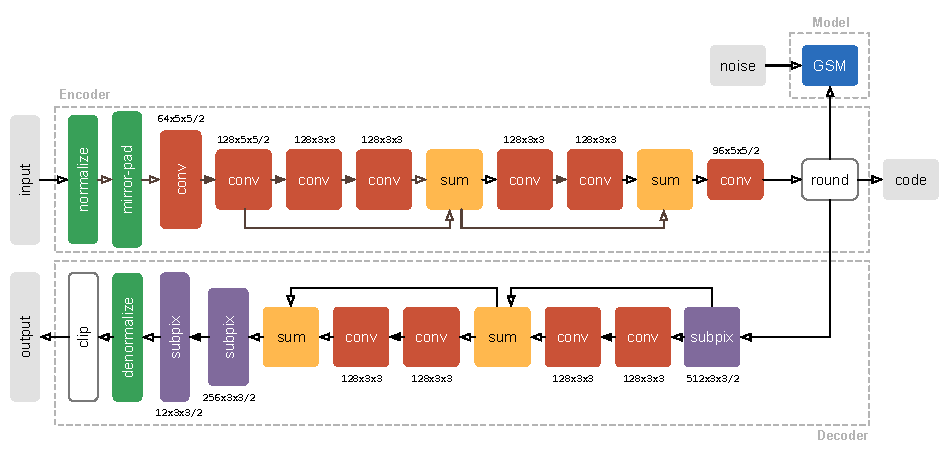
\includegraphics[width=\textwidth]{compressive_autoencoders_architecture.pdf}
  \caption{Compressive Auto-Encoder architecture used by \cite{theis2017lossy}.
    Note that for visual clarity only 2 residual blocks are displayed,
    in their experiments they used 3. They use a 6-component Gaussian Scale
    Mixture model (GSM) to model the quantization noise during the training of
    the architecture. The normalization layer performs batch normalization
    separately for each channel, denormalization is the analogous inverse
    operation. (Image taken from their \cite{theis2017lossy}.)}
  \label{fig:comp_auto_arch}
\end{figure}

\paragraph{\cite{rippel2017real}} They use a reasonably shallow architecture as well,
but also add in an additional residual connections from every layer to the last,
summing at the end. They call this
\textit{pyramidal decomposition} and \textit{interscale alignment}, with the
rationale behind it being that the residual connections extract features at
different scales, and so the latent representations can take advantage of this.
Their encoder architecture is shown in Figure \ref{fig:rippel_arch}.
\begin{figure}
  \centering 
  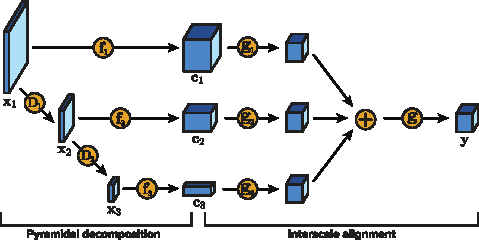
\includegraphics[width=0.7\textwidth]{rippel_architecture.pdf}
  \caption{Encoder architecture used by \cite{rippel2017real}. All circular blocks
    denote convolutions. (Image taken from \cite{rippel2017real}.)}
  \label{fig:rippel_arch}
\end{figure}
\paragraph{\cite{balle2018variational}} They extend the architecture presented in
\cite{balle2016end}, see Figure \ref{fig:balle_ladder_arch}.
In particular, the encoder and decoder remain the same,
and they add an additional stochastic layer on top of the architecture,
resembling a probabilistic ladder network (PLN) (\cite{sonderby2016train}).
The layers leading to the second level are more standard. They are still fully
convlutional with downsampling after convolutions, however, instead of GDN
they use ReLUs.
\par

\begin{figure}
  \centering 
  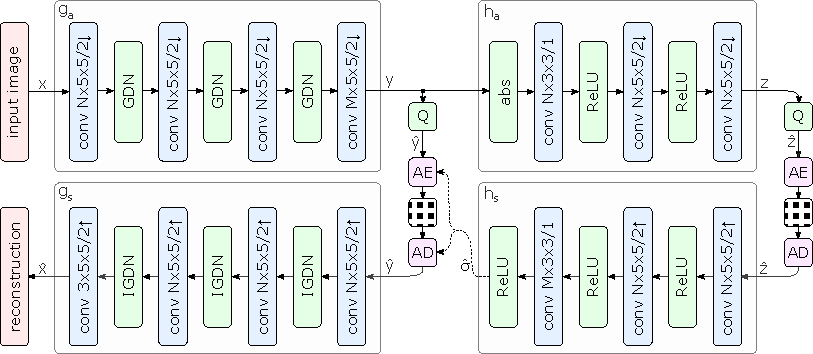
\includegraphics[width=\textwidth]{balle_ladder_architecture.pdf}
  \caption{Analysis and synthesis transforms $g_a$ and $g_s$ along with first
    level quantizer $Q(\vec{y})$ used in \cite{balle2016end}. This architecutre
    was then extended by \cite{balle2018variational} with second level analysis
    and synthesis transforms $h_a$ and $h_s$, along with second level quantizer
    $Q(\vec{z})$. This full architecture is also the basis of our model. A
    slightly strange design choice on their part is since they will wish to
    force the second stage activations to be positive (it will be predicting
    a scale parameter), instead of using an exponential or softplus
    ($\log (1 + \exp\{x\})$) activation at the end, they take the absolute value
    of the input to the first layer, and rely on the ReLUs never giving negative
    values. We are not sure if this was meant to be a computational saving, as
    taking absolute values is certainly cheaper then either of the
    aforementioned standard ways of forcing positive values, or it if it gave
    better results.
    (Image taken from \cite{balle2018variational})}
  \label{fig:balle_ladder_arch}
\end{figure}

\subsection{Addressing Non-Differentiability}
\label{sec:comp_quant}
\par
As all methods surveyed here are trained using gradient-based methods, a crucial
question that needs to be answered is how they dealt with the issue of
quantization. This is because end-to-end optimizing the transform coding
pipeline involves back-propagating gradients through the quantization step, which
yields 0 derivatives almost everywhere, stopping the learning signal.
In fact, there are two issues that need to be addressed and that we examine
below: first, the quantization operation itself, and second,
the rate estimator $H[P(\vec{z})]$ (except for \cite{rippel2017real} as they do
not use it). As we have
seen in Section \ref{sec:compression_without_quantization}, not only is there
inherent error in whatever approximation is used to circumvent the
non-differentiability of quantization, the use of quantization itself already
fundamentally limits how
effective these methods can be. A graphical representation of various continuous
relaxations / approxiamtions of quantization error can be seen in Figure
\ref{fig:quantization_models}. 
\begin{figure}
  \centering 
  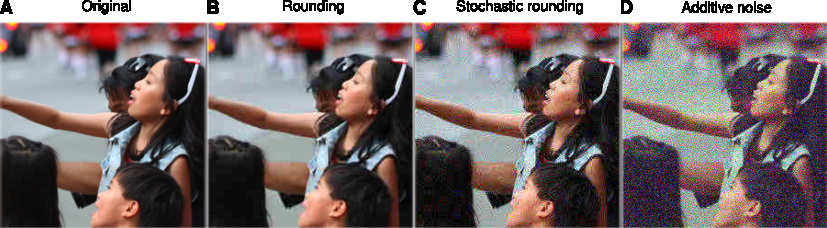
\includegraphics[width=\textwidth]{compressive_autoencoders_quant_comparison.pdf}
  \caption{Comparison of quantization error and its relaxations. \textbf{A)}
    Original image. \textbf{B)} Artifacts that result from using rounding as the
    quantizer. \textbf{C)} Stochastic rounding used by \cite{toderici2017full}.
    \textbf{D)} Uniform additive noise used by \cite{balle2016end} and
    \cite{balle2018variational}. (Image taken from \cite{theis2017lossy}.)}
  \label{fig:quantization_models}
 \end{figure}

\subsubsection{Quantization}
\par
All methods use some form of rounding $\vec{z}$ as
\begin{equation}
\label{eq:quantization_step}
  \hat{z}_i = \frac{1}{2^B}\left[2^B \times z_i\right], 
\end{equation}
for some $B$ (usually $B = 0$). Below we see what continuous relaxations are used
during training time.
 
\paragraph{\cite{balle2016end} and \cite{balle2018variational}}
They model quantization
error as dither, i.e. they replace their quantized latents
$\hat{z}_i$ by additive unifrom noise
\[
  \tilde{z}_i = z_i + \delta z_i, \quad \delta z_i \sim \Unif{0, 1}. 
\]

\paragraph{\cite{theis2017lossy}} They replace the derivative of the rounding
operation in the backpropagation chain by the constant function 1:
\[
  \frac{d}{d y} [y] = 1.
\]
This is a smooth approximation of rounding and they report that empirically it
gave good results. However, as quantization itself creates an important
bottleneck in the flow of information, it is key that only the derivative is
replaced during the backward pass and not the operation itself during the
forward pass.

\paragraph{\cite{rippel2017real}} use $B = 6$ in Eq \ref{eq:quantization_step},
however, they do not reveal their relaxation of the quantization step during
the learning phase. They cite \cite{balle2016end} and \cite{toderici2017full}
though, so our best guess is that they most likely picked a method proposed in
either one of those.

\subsubsection{Rate Estimation}
\par
As all methods but \cite{rippel2017real} under review aim to optimize
the rate-distrotion trade-off
directly, they also need to estimate the rate $H[\hat{\vec{z}}] = -\Exp{\log
  P(\hat{\vec{z}})}{P(\hat{\vec{z}})}$. Hence to model the rate during training,
they also require a distribution over the $\tilde{z}_i$s.

\paragraph{\cite{balle2016end}}
  They assume that the latents are independent, and hence they
  can model the the joint as a fully factorized distribution. They use linear
  splines to do this, whose parameters $\psi^{(i)}$ they update separately every
  $10^6$ iterations using SGD to maximize its log-likelihood on the latents,
  independently from the optimization of the rest of the model parameters.
  Then, they use this prior to replace the entropy term as
  \[
   H[\tilde{\vec{z}}] = \Exp{-\sum_i \log_2 p(z_i + \delta z_i \mid \psi^{(i)})}{}.
  \]

\paragraph{\cite{theis2017lossy}} They note that
  \[
    P(\vec{z}) = \int_{\left[-\frac{1}{2}, \frac{1}{2}\right)^M} q(\vec{z} + \vec{u}) \d \vec{u}
  \]
  for some appropriate density $q$,
  where the integral is taken over the centered $M$ dimensional hypercube.
  Then, they replace the the rate estimator with an upper bound using Jensen's
  inequality:
  \[
    -\log_2P(\vec{z}) = -\log_2\int_{\left[-\frac{1}{2}, \frac{1}{2}\right)^M} q(\vec{z} +
    \vec{u}) \d \vec{u} \leq -\int_{\left[-\frac{1}{2}, \frac{1}{2}\right)^M} \log_2q(\vec{z} +
    \vec{u}) \d \vec{u}.
  \]
  This upper bound is now differentiable. They pick Gaussian Scale Mixtures for
  $q$, with $s = 6$ components, with the mixing proportions fixed across spatial
  dimensions, which gives the negative log likelihood
  \[
    -\log_2 q(\vec{z} + \vec{u}) =
    \sum_{i, j, k} \log_2 \sum_s \pi_{k, s} \Norm{z_{k,i,j} + u_{k, i, j} \mid
    0, \sigma_{k, s}^2},
  \]
  where $i,j$ iterate through the spatial dimensions and $k$ indexes the
  filters. The integration of this in the architecture can be seen in Figure
  \ref{fig:comp_auto_arch}.  This allows them to replace the rate estimator with
  \[
    H[\tilde{\vec{z}}] = -\Exp{\log_2 q(\vec{z} + \vec{u})}{}.
  \]

  \paragraph{\cite{balle2018variational}} They us a non-parametric,
  fully factorized prior for the second stage:
  \[
    p(\tilde{\vec{z}}^{(2)} \mid \psi) =
    \prod_i \left(  p\left(\tilde{z}^{(2)}_i \mid \psi_i\right) *
      \Unif{-\frac{1}{2}, -\frac{1}{2}\right)}.
  \]
  Then, they model the first stage as dithered zero-mean Gaussians with variable
  scale depending on the second stage, thereby relaxing the initial independence
  assumption on the latent space to a more general \textit{conditional
    indepenence} assumption \cite{bishop1998latent}:
  \[
    p(\tilde{\vec{z}}^{(1)} \mid \tilde{\vec{z}}^{(2)}) = 
    \prod_i \left(  \Norm{\tilde{z}^{(1)}_i \mid 0, \tilde{\sigma}^2_i\right)*
      \Unif{-\frac{1}{2}, -\frac{1}{2}}}.
  \]
  They then replace the rate estimator similarly to \cite{balle2016end}.

\subsection{Coding}
\par
Another important part of the examined methods is the entropy coding. In particular, an
interesting caveat of entropy codes is that they tend to perform slightly worse
than the predicted rate, due to neglected constant factors in the algorithm
\cite{rissanen1981universal}. Hence, it is always more informative to present
results where the actual coding has been performed and not just the theoretical
rate reported. All examined works have implemented their own coding algorithms,
and we briefly review them here. 

\paragraph{\cite{balle2016end}} Use a context adaptive binary arithmetic coding (CABAC).
  They code dimensions in raster-scan order, which means they do not fully leverage the
  spatial dependencies between adjacent latent dimensions.
  As the authors note, this means that CABAC does not yield much improvement
  over non-adaptive artihmetic coding. 

\paragraph{\cite{theis2017lossy}} used their estimated probabilities $q(\vec{z})$ and
  used an off-the-shelf publicly available range coder to compress their latents.

\paragraph{\cite{rippel2017real}} treat each bit of their $B$-bit precision quantized
  representations individually, because they want to utilize the sparsity of
  more significant bits. They train a separate binary classifier to predict
  probabilities for each individual bit based on a set of features (they call
  it a \textit{context}) to use in an adaptive arithmetic coder. They further
  add a regularizing term during training based on the codelength of a batch to
  match a length target. This is to encourage sparsity for high-resolution, but
  low entropy images and a longer codelength for low resolution but high entropy
  images.

\paragraph{\cite{balle2018variational}} use a non-adaptive arithmetic coder as their
  entropy code. As they have two stochastic levels, with the
  first depending on the second, they have to code them sequentially. For the
  second level, they get their frequency estimates for $\hat{\vec{z}}^{(2)}$
  from the non-parametric prior:
  \[
    p(\hat{z}^{(2)}_i) =
    \int_{\hat{z}^{(2)}_i-\frac{1}{2}}^{\hat{z}^{(2)}_i+\frac{1}{2}}p(\tilde{z}_i \mid \psi_i) \d \tilde{z}_i.
  \]
  Then, on the first level, their probaibilities are given by:
  \[
    p(\hat{z}^{(1)} \mid \tilde{z}^{(2)}) = p(\hat{z}^{(1)} \mid
    \tilde{\sigma}^2_i) = 
    \int_{\hat{z}^{(1)}_i-\frac{1}{2}}^{\hat{z}^{(1)}_i + \frac{1}{2}}\Norm{\tilde{z}_i \mid 0, \tilde{\sigma}^2_i} \d \tilde{z}_i.
  \]

\subsection{Training}
\par
\cite{balle2016end}, \cite{theis2017lossy} and \cite{balle2018variational}
optimize the rate-distrotion trade-off directly,
\[
  L(\Data) = H[\hat{\vec{z}}] + \beta \Exp{d(\vec{x}, \hat{\vec{x}})}{},
\]
where the expectation is taken over training batches. This turns out to be
equivalent to maximizing the ELBO for a certain VAE, whereas \cite{rippel2017real} use a
more complex loss function, see below for details. All methods train their model
using Adam \cite{kingma2014adam}, but most do not state the number of
training epoch.

\paragraph{\cite{balle2016end}} Since they use MSE as the distance metric,
they note that their
architecture could be considered as a (somewhat
unconventional), VAE with Gaussian likelihood
\[
  p(\vec{x} \mid \tilde{\vec{z}}, \beta) =
  \Norm{\vec{x} \mid \hat{\vec{x}}, (2\beta)^{-1}\vec{1}},
\]
mean-field prior
\[
  p(\tilde{\vec{z}} \mid \psi^{1}, \hdots, \psi^{N}) =
  \prod_i p(\tilde{z}_i \mid \psi^{(i)})
\]
and mean-field posterior
\[
  q(\tilde{\vec{z}} \mid \vec{x}) =
  \prod_i \Unif{\tilde{z}_i \mid z_i, 1},
\]
where $\Unif{\tilde{z}_i \mid z_i, 1},$ is the uniform distribution centered
on $z_i$ of width 1. They used learning rate decay during training.

\paragraph{\cite{theis2017lossy}}
  They performed the training incrementally, in the sense that they masked most
  latents at the start, such that their contribution to the loss was 0. Then, as
  the training performance saturated, they unmasked them incrementally. They
  also used learning rate decay during training.

\paragraph{\cite{rippel2017real}} They use a complex loss function, with an MS-SSIM
distrotion cost, a code length regularization term (not equivalent to the rate
term) as well as an adversarial loss term. In their adversarial setup they feed
ground truth, reconstruction pairs to the discriminator, where they shuffle the
images in the pair with probability $\frac12$ and their discriminator was
trained to predict which image was the reconstruction. Their setup can be seen
in Figure \ref{fig:rippel_pipeline}. To stabilize the
adversarial training procedure, they also introduce an adaptive learning signal
scheduler, preventing any of the signals from dominating the total.
\begin{figure}
  \centering 
  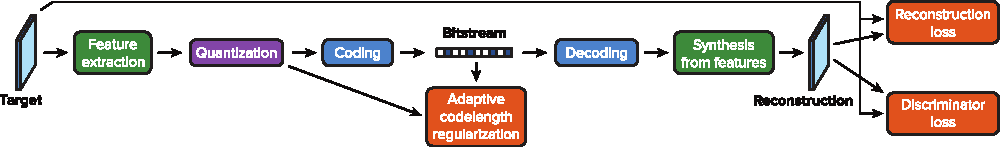
\includegraphics[width=\textwidth]{rippel_pipeline.pdf}
  \caption{Compression pipeline used by \cite{rippel2017real}. The red boxes
    show the terms used in their loss function. (Image taken from \cite{rippel2017real}.)}
  \label{fig:rippel_pipeline}
\end{figure}

\paragraph{\cite{balle2018variational}} In the same vein as they laid out their
  VAE-based training objective in \cite{balle2016end}, the data log-likelihood
  term stays, but now the regularizing term is the KL divergence between the
  joint posterior $q(\tilde{\vec{z}}^{(1)}, \tilde{\vec{z}}^{(2)} \mid \vec{x})$
  and the joint prior 
  $q(\tilde{\vec{z}}^{(1)}, \tilde{\vec{z}}^{(2)})$. Here, as due to the
  dithering assumption, the joint posterior works out to be
  \[
    q\left(\tilde{\vec{z}}^{(1)}, \tilde{\vec{z}}^{(2)} \mid \vec{x}\right) =
    \prod_i \Unif{\tilde{z}^{(1)}_i \mid \hat{z}^{(1)}, 1} \cdot
    \prod_i \Unif{\tilde{z}^{(2)}_i \mid \hat{z}^{(2)}, 1}.
  \]
  \par
  Then, taking the KL between these, the full traning objective works out to be
  \begin{equation}
    \label{eq:balle_var_train_objective}
    L = \Exp{ -\sum_i \log_2 p(\tilde{z}^{(2)}_i \mid \psi^{(i)}) 
      -\sum_i \log_2 p(\tilde{z}^{(1)}_i \mid \tilde{\sigma}^2_i) +
      \beta d(\vec{x}, \hat{\vec{x}})}{}.
  \end{equation}
  Eq \ref{eq:balle_var_train_objective} is important from our prespective, as
  it will be
  directly translated to our learning objective.
  \par
  They train 32 models, half using the architecture from \cite{balle2016end} and
  half using the current one, half optimized for MSE and half of MS-SSIM, with 8
  different $\beta$s. They report that neither batch normalization nor learning
  rate decay gave better results, which they attribute to GDN.

\subsection{Evaluation}
\par
As mentioned at the end of Section \ref{sec:related_works_datasets}, all
methods were tested on the Kodak dataset (\cite{kodakdataset}). All authors
report the (interpolated) rate-distrotion curves achieved by their models. All
methods report the curves using PSNR (\cite{psnr}) as the distrotion metric as
well as MS-SSIM (\cite{msssim}), except for \cite{rippel2017real}, who only
report MS-SSIM. Based on these reported curves, the current state-of-the-art in
neural compression is set by \cite{balle2018variational}. 
\par
An important issue raised in \cite{balle2016end} and \cite{balle2018variational}
is how aggregate results over should be reported, or whether reporting such
figures is meaninful in the first place. This is because since models were
trained on different datasets, with different model design philosophies, there
might be significant fluctuation in the comparative model performance between
individual images. Furthermore, averaging results achieved by classical methods
that were not directly optimized for the rate-distrotion trade-off (virtually
all of them) might lead to inconsistent results even on the same image, depending on what settings were used to achieve
a given bitrate. Hence, they argue that the efficiency of the methods should
be examined on individual images instead. This is also the philosophy we follow,
and hence we will be reporting model performances on individual images.
%!TEX root = ../thesis.tex
%*******************************************************************************
%****************************** Second Chapter *********************************
%*******************************************************************************

\chapter{Related Works}
\label{chapter:related_works}

\graphicspath{{../img/related_works/}}

\par
In this chapter, we give a brief overview of the history of ML-based image
compression. Then, we focus on recent advances in lossy neural image compression
and describe and compare them against each other.

\section{Machine Learning-based Image Compression}
\par
Neural image compression goes back to at least as far as the early 1980s
(\cite{mougeot1991image}, \cite{jiang1999image}). These methods very closely
resemble in high-level structure to contemporary methods, in that they were
designed as transform coding methods. In particular, virtually all early methods
used some flavour of linear auto-encoders (LAEs, no non-linearities applied on
the hidden layer), with a single-layer encoder and
decoder (\cite{jiang1999image}). As convolutional layers had not yet been
available back then, all architectures were fully connected
and relied on splitting up images into equal-sized blocks and feeding them
block-by-block to the LAE. Most methods optimized the MSE between the
reconstruction and the original image, although different learning objectives
were also explored (\cite{mougeot1991image}). Furthermore, the issue of
quantization was not formally addressed. While the pipeline was to quantize the hidden
layer activations of the LAE, no explicit treatment of the distortion introduced
by quantization was given (\cite{jiang1999image}).

\par
A notable early example of a non-neural ML-based practical compression method
is DjVu (\cite{bottou1998high}), which focused on segmenting foreground and
background in documents and using K-means clustering to for the analysis
transforming followed by entropy coding the background.

\par 
More recently, the work of \cite{denton2015deep}, \cite{gregor2015draw} focused
on discovering compressive representations using auto-encoders on low-resolution
images, using datasets such as CIFAR-10 (\cite{krizhevsky2009learning}).
\cite{toderici2015variable} proposed an RNN-based auto-encoder for compressing $32
\times 32$ thumbnails and outperformed classical methods such as JPEG and WebP
on these sizes. Their method has been later extended in \cite{toderici2017full}
for large-scale images. 

\section{Comparison of Recent Works}
\label{sec:lit_comparison}
\par
In this section, we focus on compression methods that allow for the compression
of arbitrary-sized images. The most notable recent works in this area (that we
are aware of) are \cite{balle2016end}, \cite{toderici2017full}, \cite{theis2017lossy},
\cite{rippel2017real}, \cite{balle2018variational}, \cite{johnston2018cvpr} and
\cite{mentzer2018cvpr}. Of these, \cite{balle2016end}, \cite{theis2017lossy},
\cite{rippel2017real} and \cite{balle2018variational} are closest to our work and
thus we present a review of these below.

\paragraph{Note on Notation:} In this chapter, we denote the output of the
encoders by $\vec{z}$, their quantized values by $\hat{\vec{z}}$ and their
continuous relaxations by $\tilde{\vec{z}}$.

\subsection{Datasets and Input Pipelines}
\label{sec:related_works_datasets}
\par
Somewhat surprisingly, it appears that there appears to be no canonical dataset
yet for general lossy neural image compression. Such a dataset should be
comprised of a set of high-resolution, variable-sized losslessly
encoded colour images, although the CLIC Dataset (\cite{clic2018}) seems to be
an emerging one. Perhaps the reason is that generally in other domains, such as
image-based classification, cropping and rescaling images can effectively
side-step the need to deal with variable-sized images. However, when it comes
to compression, if we hope to build anything useful, side-stepping the size
issue is not an option.

\paragraph{\cite{balle2016end}} trained on 6507 images, selected from ImageNet
\cite{deng2009imagenet}. They removed images with excessive saturation and
since their method is based on dithering, they added uniform noise to the
remaining images to imitate the noise introduced by quantization. Finally,
they downsampled and cropped images to be $256 \times 256$ pixels in size.
They only kept images while resampling factor was 0.75 or less, to
avoid high-frequency noise.

\paragraph{\cite{theis2017lossy}} used 434 high-resolution images from \url{flickr.com}
under the creative commons license. As \texttt{flickr} store its images as
JPEGs, they downsampled all images to be below $1536 \times 1536$ in
resolution and saved them as PNGs to reduce the effects of the lossy
compression. Then, they extracted several $128 \times 128$ patches from each
image and trained on those.

\paragraph{\cite{rippel2017real}} took images from the Yahoo Flickr Creative Commons
100 Million dataset, with $128 \times 128$ patches randomly sampled from the
images. They do not state whether they used the whole dataset or just a
subset, neither do they describe further preprocessing steps.

\paragraph{\cite{balle2018variational}} scraped $\approx$ 1 million colour JPEG images
of dimensions at most $3000 \times 5000$. They filtered out images with
excessive saturation similarly to \cite{balle2016end}. They also
downsampled images by random factors such that the image's height and width
stayed above 640 and 1200 pixels, respectively. Finally, they use several
randomly cropped $256 \times 256$ pixel patches extracted from each image.

\paragraph{}
A clear trend is downsampling large, lossy-encoded images to get rid of the
compression artefacts as an easy way of obtaining reasonable ``approximations''
of losslessly encoded images. Another trend is that (as we see in the next
section) since all architectures are fully convolutional, it is sufficient to
train on small image patches to train the convolution kernels to speed up
training, as well as to heavily ``increase'' the training set size.

\paragraph{Datasets for testing}
In contrast to the lack of datasets for training, all authors have used standard
datasets for testing their methods, taken from classical lossy image
compression research. These are the Kodak (\cite{kodakdataset}) and Tecnick
(\cite{asuni2014testimages}) datasets. For our results to be comparable
to these methods, we have also decided to test our method on the Kodak dataset.

\subsection{Architectures}
\par
This is the most diverse aspect of recent approaches, and so we will only
discuss them on a high level. We incorporated ideas from all of these papers
as well as others into our work, we discuss these in Chapter \ref{chapter:method}. All
architectures (including ours) realize a form of non-linear transform
coding. This means all architectures will have an \textit{analysis transform} or
\textit{encoder}, and a \textit{synthesis transform} or \textit{decoder} (see
Section \ref{sec:transform_coding}), both of whose parameters the methods learn
using gradient descent.
\par
All methods
achieve the ability to deal with arbitrary-sized images by only utilizing
convolutional and deconvolutional layers as their linear transformations. This
leads to the very natural consequence that the number of latent dimensions, and
thus the latent code length increases linearly in the number of pixels of the
input image. They all utilise downsampling after some convolutions.
Every work that gives details
on how they perform downsampling do it by using a stride larger than 1 on the
convolutions, and it is reasonable to assume that the rest do it likewise.
Padding and convolution mode is generally not discussed except in
\cite{theis2017lossy}, but we believe all other methods use one of the two ways
they present, namely zero-padded or mirror-padded convolutions in \texttt{same}
mode. The further details of each work are detailed below.

\paragraph{\cite{balle2016end}} They build a relatively shallow autoencoder (5
layers) (Shown in the left half of Figure \ref{fig:balle_ladder_arch}).
They propose their own activation function, custom-tailored for image
compression. These non-linearities are a form of adaptive local gain control
for the images, called Generalized Divisive Normalization (GDN). At the $k$th layer for
channel $i$ at position $(m, n)$, for input $w_i^{(k)}(m, n)$, the GDN
transform is defined as
\begin{equation}
  \label{eq:gdn_def}
  u_i^{(k + 1)}(m, n) = \frac{w_i^{(k)}(m, n)}{
    \left( \beta_{k, i} + \sum_j \gamma_{k, i, j}
      \left( w_{j}^{(k)}(m, n)\right)^2 \right)}.
\end{equation}
Its approximate inverse, IGDN for input $\hat{u}_i^{(k)}(m, n)$ is defined as
\begin{equation}
  \label{eq:igdn_def}
  \hat{w}_i^{(k)}(m, n) = \hat{u}_i^{(k)}(m, n) \cdot \left(
    \hat{\beta}_{k, i} + \sum_{j} \hat{\gamma}_{k, i, j} \left(
      \hat{u}_j^{(k)}(m, n)\right)^2 \right)^{\frac{1}{2}}.
\end{equation}
Here, the set $\beta_{k, i}, \gamma_{i, j, k}, \hat{\beta}_{k, i},
\hat{\gamma}_{i, j, k}$ are learned during training and fixed at test time.

\paragraph{\cite{theis2017lossy}} They define a Compressive Autoencoder (CAE) as a regular
autoencoder with the quantization step between the encoding and decoding step.
(In this sense, the architectures of \cite{balle2016end} and
\cite{balle2018variational} are also CAEs.) They mirror pad the input first
and then they follow it up by a deep, fully convolutional, residual
architecture \cite{he2016deep}. They use valid convolutions and downsample by
using a stride of 2. Between convolutions they use leaky ReLUs as
nonlinearities, which are defined as 
\[
  f_\alpha(x) = \max\{x, \alpha x\}, \quad \alpha \in [0, 1].
\]
The decoder mirrors the encoder. When upsampling is required, they use what
they term \textit{subpixel} convolutions, where they perform a regular
convolution operation with an increased number of filters, and then reshape
the resulting tensor into one with a larger spatial extent but fewer channels.
Their architecture can be seen in Figure \ref{fig:comp_auto_arch}.
\begin{figure}
  \centering 
  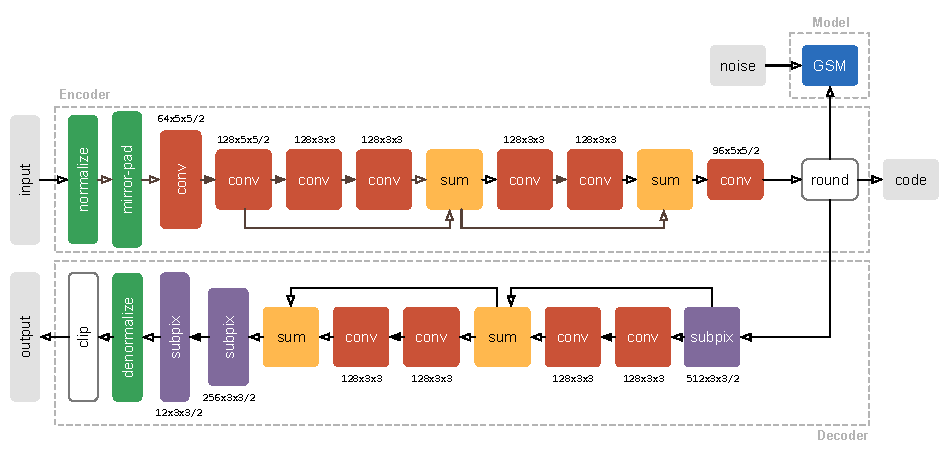
\includegraphics[width=\textwidth]{compressive_autoencoders_architecture.pdf}
  \caption[Compressive Auto-Encoder architecture used by \cite{theis2017lossy}.]
  {Compressive Auto-Encoder architecture used by \cite{theis2017lossy}.
    Note that for visual clarity only 2 residual blocks are displayed,
    in their experiments they used 3. They use a 6-component Gaussian Scale
    Mixture model (GSM) to model the quantization noise during the training of
    the architecture. The normalization layer performs batch normalization
    separately for each channel, denormalization is the analogous inverse
    operation. (Image is taken from their \cite{theis2017lossy}.)}
  \label{fig:comp_auto_arch}
\end{figure}

\paragraph{\cite{rippel2017real}} They use a reasonably shallow architecture as well,
but also add in additional residual connections from every layer to the last,
summing at the end. They call this
\textit{pyramidal decomposition} and \textit{interscale alignment}, with the
rationale behind it being that the residual connections extract features at
different scales, and so the latent representations can take advantage of this.
Their encoder architecture is shown in Figure \ref{fig:rippel_arch}.
\begin{figure}
  \centering 
  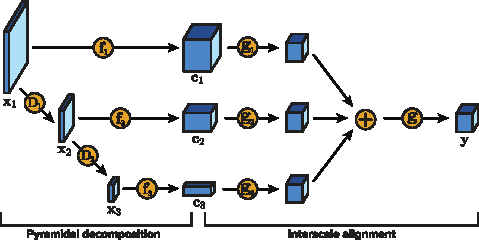
\includegraphics[width=0.7\textwidth]{rippel_architecture.pdf}
  \caption[Encoder architecture used by \cite{rippel2017real}.]
  {Encoder architecture used by \cite{rippel2017real}. All circular blocks
    denote convolutions. (Image taken from \cite{rippel2017real}.)}
  \label{fig:rippel_arch}
\end{figure}
\paragraph{\cite{balle2018variational}} They extend the architecture presented in
\cite{balle2016end}, see Figure \ref{fig:balle_ladder_arch}.
In particular, the encoder and decoder remain the same,
and they add one more stochastic layer on top of the architecture,
resembling a probabilistic ladder network (PLN) (\cite{sonderby2016train}).
The layers leading to the second level are more standard. They are still fully
convolutional with downsampling after convolutions, however, instead of GDN
they use ReLUs.
\par

\begin{figure}
  \centering 
  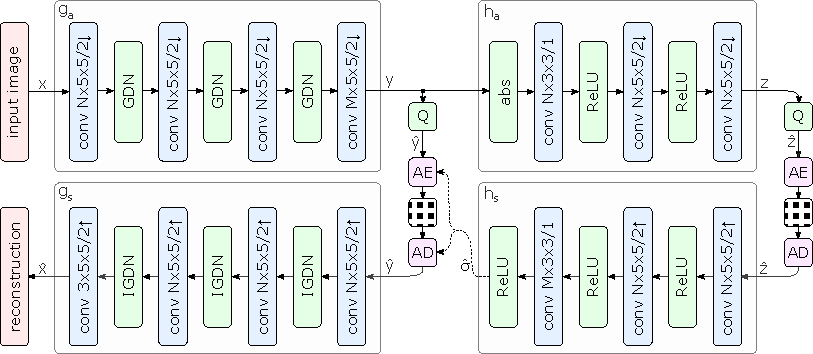
\includegraphics[width=\textwidth]{balle_ladder_architecture.pdf}
  \caption[Architecture used by \cite{balle2018variational}.]
  {Analysis and synthesis transforms $g_a$ and $g_s$ along with first
    level quantizer $Q(\vec{y})$ used in \cite{balle2016end}. This architecture
    was then extended by \cite{balle2018variational} with second-level analysis
    and synthesis transforms $h_a$ and $h_s$, along with second level quantizer
    $Q(\vec{z})$. This full architecture is also the basis of our model. A
    slightly strange design choice on their part is since they will wish to
    force the second stage activations to be positive (it will be predicting
    a scale parameter), instead of using an exponential or softplus
    ($\log (1 + \exp\{x\})$) activation at the end, they take the absolute value
    of the input to the first layer, and rely on the ReLUs never giving negative
    values. We are not sure if this was meant to be a computational saving, as
    taking absolute values is certainly cheaper then either of the
    aforementioned standard ways of forcing positive values or it if it gave
    better results.
    (Image is taken from \cite{balle2018variational})}
  \label{fig:balle_ladder_arch}
\end{figure}

\subsection{Addressing Non-Differentiability}
\label{sec:comp_quant}
\par
As all methods surveyed here are trained using gradient-based methods, a crucial
question that needs to be answered is how they dealt with the issue of
quantization. This is because end-to-end optimizing the transform coding
pipeline involves back-propagating gradients through the quantization step, which
yields 0 derivatives almost everywhere, stopping the learning signal.
Two issues that need to be addressed and that we examine
below: first, the quantization operation itself, and second,
the rate estimator $H[P(\vec{z})]$ (except for \cite{rippel2017real} as they do
not use it). As we have
seen in Section \ref{sec:compression_without_quantization}, not only is there
an inherent error in whatever approximation is used to circumvent the
non-differentiability of quantization, the use of quantization itself already
fundamentally limits how
effective these methods can be. A graphical representation of various continuous
relaxations / approximations of quantization error can be seen in Figure
\ref{fig:quantization_models}. 
\begin{figure}
  \centering 
  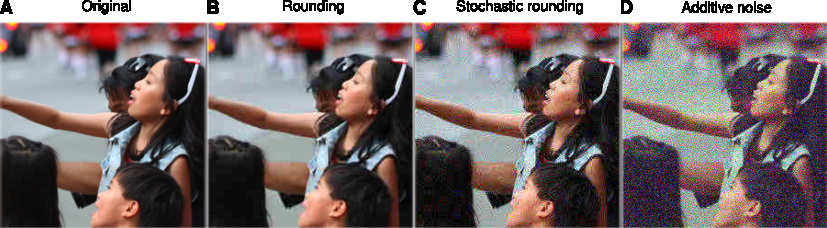
\includegraphics[width=\textwidth]{compressive_autoencoders_quant_comparison.pdf}
  \caption[Comparison of quantization error and its relaxations.]
  {Comparison of quantization error and its relaxations. \textbf{A)}
    Original image. \textbf{B)} Artefacts that result from using rounding as the
    quantizer. \textbf{C)} Stochastic rounding used by \cite{toderici2017full}.
    \textbf{D)} Uniform additive noise used by \cite{balle2016end} and
    \cite{balle2018variational}. (Image taken from \cite{theis2017lossy}.)}
  \label{fig:quantization_models}
 \end{figure}

\subsubsection{Quantization}
\par
All methods use some form of rounding $\vec{z}$ as
\begin{equation}
\label{eq:quantization_step}
  \hat{z}_i = \frac{1}{2^B}\left[2^B \times z_i\right], 
\end{equation}
for some $B$ (usually $B = 0$). Below we see what continuous relaxations are used
during training time.
 
\paragraph{\cite{balle2016end} and \cite{balle2018variational}}
They model quantization
error as dither, i.e. they replace their quantized latents
$\hat{z}_i$ by additive uniform noise
\[
  \tilde{z}_i = z_i + \delta z_i, \quad \delta z_i \sim \Unif{0, 1}. 
\]

\paragraph{\cite{theis2017lossy}} They replace the derivative of the rounding
operation in the backpropagation chain by the constant function 1:
\[
  \frac{d}{d y} [y] = 1.
\]
This is a smooth approximation of rounding and they report that empirically it
gave good results. However, as quantization itself creates an important
bottleneck in the flow of information, it is key that only the derivative is
replaced during the backward pass and not the operation itself during the
forward pass.

\paragraph{\cite{rippel2017real}} use $B = 6$ in Eq \ref{eq:quantization_step},
however, they do not reveal their relaxation of the quantization step during
the learning phase. They cite \cite{balle2016end} and \cite{toderici2017full}
though, so our best guess is that they most likely picked a method proposed in
either one of those.

\subsubsection{Rate Estimation}
\par
As all methods but \cite{rippel2017real} under review aim to optimize
the rate-distortion trade-off
directly, they also need to estimate the rate $H[\hat{\vec{z}}] = -\Exp{\log
  P(\hat{\vec{z}})}{P(\hat{\vec{z}})}$. Hence to model the rate during training,
they also require a distribution over the $\tilde{z}_i$s.

\paragraph{\cite{balle2016end}}
  They assume that the latents are independent, and hence they
  can model the joint as a fully factorized distribution. They use linear
  splines to do this, whose parameters $\psi^{(i)}$ they update separately every
  $10^6$ iterations using SGD to maximize its log-likelihood on the latents,
  independently from the optimization of the rest of the model parameters.
  Then, they use this prior to replace the entropy term as
  \[
   H[\tilde{\vec{z}}] = \Exp{-\sum_i \log_2 p(z_i + \delta z_i \mid \psi^{(i)})}{}.
  \]

\paragraph{\cite{theis2017lossy}} They note that
  \[
    P(\vec{z}) = \int_{\left[-\frac{1}{2}, \frac{1}{2}\right)^M} q(\vec{z} + \vec{u}) \d \vec{u}
  \]
  for some appropriate density $q$,
  where the integral is taken over the centred $M$ dimensional hypercube.
  Then, they replace the rate estimator with an upper bound using Jensen's
  inequality:
  \[
    -\log_2P(\vec{z}) = -\log_2\int_{\left[-\frac{1}{2}, \frac{1}{2}\right)^M} q(\vec{z} +
    \vec{u}) \d \vec{u} \leq -\int_{\left[-\frac{1}{2}, \frac{1}{2}\right)^M} \log_2q(\vec{z} +
    \vec{u}) \d \vec{u}.
  \]
  This upper bound is now differentiable. They pick Gaussian Scale Mixtures for
  $q$, with $s = 6$ components, with the mixing proportions fixed across spatial
  dimensions, which gives the negative log likelihood
  \[
    -\log_2 q(\vec{z} + \vec{u}) =
    \sum_{i, j, k} \log_2 \sum_s \pi_{k, s} \Norm{z_{k,i,j} + u_{k, i, j} \mid
    0, \sigma_{k, s}^2},
  \]
  where $i,j$ iterate through the spatial dimensions and $k$ indexes the
  filters. The integration of this in the architecture can be seen in Figure
  \ref{fig:comp_auto_arch}.  This allows them to replace the rate estimator with
  \[
    H[\tilde{\vec{z}}] = -\Exp{\log_2 q(\vec{z} + \vec{u})}{}.
  \]

  \paragraph{\cite{balle2018variational}} They us a non-parametric,
  fully factorized prior for the second stage:
  \[
    p(\tilde{\vec{z}}^{(2)} \mid \psi) =
    \prod_i \left(  p\left(\tilde{z}^{(2)}_i \mid \psi_i\right) *
      \Unif{-\frac{1}{2}, -\frac{1}{2}\right)}.
  \]
  Then, they model the first stage as dithered zero-mean Gaussians with variable
  scale depending on the second stage, thereby relaxing the initial independence
  assumption on the latent space to a more general \textit{conditional
    independence} assumption \cite{bishop1998latent}:
  \[
    p(\tilde{\vec{z}}^{(1)} \mid \tilde{\vec{z}}^{(2)}) = 
    \prod_i \left(  \Norm{\tilde{z}^{(1)}_i \mid 0, \tilde{\sigma}^2_i\right)*
      \Unif{-\frac{1}{2}, -\frac{1}{2}}}.
  \]
  They then replace the rate estimator similarly to \cite{balle2016end}.

\subsection{Coding}
\par
Another important part of the examined methods is entropy coding. In particular, an
interesting caveat of entropy codes is that they tend to perform slightly worse
than the predicted rate, due to neglected constant factors in the algorithm
\cite{rissanen1981universal}. Hence, it is always more informative to present
results where the actual coding has been performed and not just the theoretical
rate reported. All examined works have implemented their own coding algorithms,
and we briefly review them here. 

\paragraph{\cite{balle2016end}} Use a context adaptive binary arithmetic coding (CABAC).
  They code dimensions in raster-scan order, which means they do not fully leverage the
  spatial dependencies between adjacent latent dimensions.
  As the authors note, this means that CABAC does not yield much improvement
  over non-adaptive arithmetic coding. 

\paragraph{\cite{theis2017lossy}} used their estimated probabilities $q(\vec{z})$ and
  used an off-the-shelf publicly available range coder to compress their latents.

\paragraph{\cite{rippel2017real}} treat each bit of their $B$-bit precision quantized
  representations individually because they want to utilize the sparsity of
  more significant bits. They train a separate binary classifier to predict
  probabilities for individual bits based on a set of features (they call
  it a \textit{context}) to use in an adaptive arithmetic coder. They further
  add a regularizing term during training based on the code length of a batch to
  match a length target. This is to encourage sparsity for high-resolution, but
  low entropy images and a longer codelength for low resolution but high entropy
  images.

\paragraph{\cite{balle2018variational}} use a non-adaptive arithmetic coder as their
  entropy code. As they have two stochastic levels, with the
  first depending on the second, they have to code them sequentially. For the
  second level, they get their frequency estimates for $\hat{\vec{z}}^{(2)}$
  from the non-parametric prior:
  \[
    p(\hat{z}^{(2)}_i) =
    \int_{\hat{z}^{(2)}_i-\frac{1}{2}}^{\hat{z}^{(2)}_i+\frac{1}{2}}p(\tilde{z}_i \mid \psi_i) \d \tilde{z}_i.
  \]
  Then, on the first level, their probabilities are given by:
  \[
    p(\hat{z}^{(1)} \mid \tilde{z}^{(2)}) = p(\hat{z}^{(1)} \mid
    \tilde{\sigma}^2_i) = 
    \int_{\hat{z}^{(1)}_i-\frac{1}{2}}^{\hat{z}^{(1)}_i + \frac{1}{2}}\Norm{\tilde{z}_i \mid 0, \tilde{\sigma}^2_i} \d \tilde{z}_i.
  \]

\subsection{Training}
\par
\cite{balle2016end}, \cite{theis2017lossy} and \cite{balle2018variational}
optimize the rate-distortion trade-off directly,
\[
  L(\Data) = H[\hat{\vec{z}}] + \beta \Exp{d(\vec{x}, \hat{\vec{x}})}{},
\]
where the expectation is taken over training batches. This turns out to be
equivalent to maximizing the ELBO for a certain VAE, whereas \cite{rippel2017real} use a
more complex loss function, see below for details. All methods train their model
using Adam \cite{kingma2014adam}, but most do not state the number of
training epoch.

\paragraph{\cite{balle2016end}} Since they use MSE as the distance metric,
they note that their
architecture could be considered as a (somewhat
unconventional), VAE with Gaussian likelihood
\[
  p(\vec{x} \mid \tilde{\vec{z}}, \beta) =
  \Norm{\vec{x} \mid \hat{\vec{x}}, (2\beta)^{-1}\vec{1}},
\]
mean-field prior
\[
  p(\tilde{\vec{z}} \mid \psi^{1}, \hdots, \psi^{N}) =
  \prod_i p(\tilde{z}_i \mid \psi^{(i)})
\]
and mean-field posterior
\[
  q(\tilde{\vec{z}} \mid \vec{x}) =
  \prod_i \Unif{\tilde{z}_i \mid z_i, 1},
\]
where $\Unif{\tilde{z}_i \mid z_i, 1},$ is the uniform distribution centred
on $z_i$ of width 1. They used learning rate decay during training.

\paragraph{\cite{theis2017lossy}}
  They performed the training incrementally, in the sense that they masked most
  latents at the start, such that their contribution to the loss was 0. Then, as
  the training performance saturated, they unmasked them incrementally. They
  also used learning rate decay during training.

\paragraph{\cite{rippel2017real}} They use a complex loss function, with an MS-SSIM
distortion cost, a code length regularization term (not equivalent to the rate
term) as well as an adversarial loss term. In their adversarial setup, they feed
ground truth, reconstruction pairs to the discriminator, where they shuffle the
images in the pair with probability $\frac12$ and their discriminator was
trained to predict which image was the reconstruction. Their setup can be seen
in Figure \ref{fig:rippel_pipeline}. To stabilize the
adversarial training procedure, they also introduce an adaptive learning signal
scheduler, preventing any of the signals from dominating the total.
\begin{figure}
  \centering 
  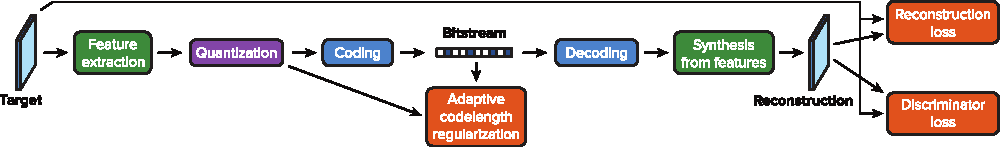
\includegraphics[width=\textwidth]{rippel_pipeline.pdf}
  \caption[Compression pipeline used by \cite{rippel2017real}.]
  {Compression pipeline used by \cite{rippel2017real}. The red boxes
    show the terms used in their loss function. (Image is taken from
    \cite{rippel2017real}.)}
  \label{fig:rippel_pipeline}
\end{figure}

\paragraph{\cite{balle2018variational}} In the same vein as they laid out their
  VAE-based training objective in \cite{balle2016end}, the data log-likelihood
  term stays, but now the regularizing term is the KL divergence between the
  joint posterior $q(\tilde{\vec{z}}^{(1)}, \tilde{\vec{z}}^{(2)} \mid \vec{x})$
  and the joint prior 
  $q(\tilde{\vec{z}}^{(1)}, \tilde{\vec{z}}^{(2)})$. Here, as due to the
  dithering assumption, the joint posterior works out to be
  \[
    q\left(\tilde{\vec{z}}^{(1)}, \tilde{\vec{z}}^{(2)} \mid \vec{x}\right) =
    \prod_i \Unif{\tilde{z}^{(1)}_i \mid \hat{z}^{(1)}, 1} \cdot
    \prod_i \Unif{\tilde{z}^{(2)}_i \mid \hat{z}^{(2)}, 1}.
  \]
  \par
  Then, taking the KL between these, the full traning objective works out to be
  \begin{equation}
    \label{eq:balle_var_train_objective}
    L = \Exp{ -\sum_i \log_2 p(\tilde{z}^{(2)}_i \mid \psi^{(i)}) 
      -\sum_i \log_2 p(\tilde{z}^{(1)}_i \mid \tilde{\sigma}^2_i) +
      \beta d(\vec{x}, \hat{\vec{x}})}{}.
  \end{equation}
  Eq \ref{eq:balle_var_train_objective} is important from our perspective, as
  it will be
  directly translated to our learning objective.
  \par
  They train 32 models, half using the architecture from \cite{balle2016end} and
  the other half using the current one, half optimized for MSE and the other
  half of MS-SSIM, with 8
  different $\beta$s. They report that neither batch normalization nor learning
  rate decay gave better results, which they attribute to GDN.

\subsection{Evaluation}
\par
As mentioned at the end of Section \ref{sec:related_works_datasets}, all
methods were tested on the Kodak dataset (\cite{kodakdataset}). All authors
report the (interpolated) rate-distortion curves achieved by their models. All
methods report the curves using PSNR (\cite{psnr}) as the distortion metric as
well as MS-SSIM (\cite{msssim}), except for \cite{rippel2017real}, who only
report MS-SSIM. Based on these reported curves, the current state-of-the-art in
neural compression is set by \cite{balle2018variational}. 
\par
An important issue raised in \cite{balle2016end} and \cite{balle2018variational}
is how aggregate results over should be reported, or whether reporting such
figures is meaningful in the first place. This is because since models were
trained on different datasets, with different model design philosophies, there
might be significant fluctuation in the comparative model performance between
individual images. Furthermore, averaging results achieved by classical methods
that were not directly optimized for the rate-distortion trade-off (virtually
all of them) might lead to inconsistent results even on the same image, depending on what settings were used to achieve
a given bitrate. Hence, they argue that the efficiency of the methods should
be examined on individual images instead. This is also the philosophy we follow,
and hence we will be reporting model performances on individual images.
%!TEX root = ../thesis.tex
%*******************************************************************************
%****************************** Third Chapter **********************************
%*******************************************************************************

\chapter{Method}
\label{chapter:method}

% **************************** Define Graphics Path **************************
\graphicspath{{../img/thesis/}{../img/plots/vae_latents/}{../img/related_works/}}

\par
In this chapter, we describe the models we use to demonstarte the efficiency of the
general lossy compression framework developed in Section
\ref{sec:compression_without_quantization}. We begin by describing the input
pipeline, followed by our model architectures and their training procedure. We
then present 3 tractable, coded sampling algorithms that can be used within our
framework.

Based on our framework, at a high level our image compression algorithm is as
follows:

\begin{framed}
\begin{enumerate}
\item Pick an appropriate VAE-based architecture (Probabilistic Ladder Networks
  (PLNs) in our case) for image reconstruction. (Section \ref{sec:architectures})

\item Train the model on a reasonably selected dataset for this task. (Sections
  \ref{sec:dataset_preproc} and \ref{sec:architectures})

\item Once the VAE is trained, given a new image
  $\vec{x}$, we can use the latent posterior $q(\vec{z} \mid \vec{x})$ and
  prior $p(\vec{z})$ for our coded sampling algorithm. (Section
  \ref{sec:coded_sampling})

\item We may consider to use entropy codes to further increase the efficiency of
  our coding, if appropriate. 

\end{enumerate}
\end{framed}

\par
A rather pleasing aspect of this is the modularity that is allowed by the
removal of quantization from the training pipeline: our method is reusable with
virtually any regular VAE architecture, which opens up the possibility of
creating efficient compression algorithms for any domain where a VAE can be used
to reconstruct the objects of interest. 

\section{Dataset and Preprocessing}
\label{sec:dataset_preproc}
\par
We trained our models on the CLIC 2018 dataset (\cite{clic2018}), as it seemed
sufficiently extensive for our project. It was also curated for an image
compression challenge, and thus ``bad'' images have been
filtered out, which reduced the amount of preprocessing required on our side.
\par
The dataset contains high-resolution PNG encoded photographs, 585 in the
training set and 41 photos in the validation set. The test set is not
publicly available, as it was reserved for the competition. 
To make training tractable, similarly to previous works, we randomly extracted
$256 \times 256$ pixel patches from each image. The number of patches $P$ was
based on their size of the image, according to the formula
\[
  P(W, H) = C \times \left \lfloor \frac{W}{256} \right \rfloor \times
  \left \lfloor \frac{H}{256} \right \rfloor,
\]
where $W, H$ are the width and height of the current image, respectively and $C$
is an integer constant we set. We used $C = 15$, which yielded us a training set
of 93085 patches.
\par
We note that all image data we used for learning was in RGB format. It is
possible to achieve better compression rates using the YCbCr format
(\cite{balle2016end}, \cite{rippel2017real}), however, for simplicity's sake as
well as due to time constraints we leave investigating this for later work.
\section{Architectures}
\label{sec:architectures}
\par
In this section we describe the various architectures that we experimented with.
The basis of all our architectures were inspired by the ones used in
\cite{balle2016end} and \cite{balle2018variational}. In particular, we use the
General Divisive Normalization (GDN) layer for encoding and its approximate
inverse, the IGDN layer for decoding (\cite{balle2015density}, \cite{balle2016end}).

\subsection{VAEs}
\label{sec:method_vaes}
\par
As a baseline, we started by replicating the exact architecture
presented in \cite{balle2016end}, but using a Gaussian prior and posterior
instead. We chose mirror padding with our convolutions, as it is standard
for in this setting (\cite{theis2017lossy}). Luckily, the most
error-prone part, the implementation of the GDN and IGDN layers was already
available in \texttt{Tensorflow}\footnotemark.

\par While VAEs are by now fairly standard and we assume that the reader is at
least somewhat familiar with them, our later models build on them and are
non-standard, hence it is useful to briefly go over them and introduce
notation that we extend in the following sections.

\footnotetext{\url{https://www.tensorflow.org/api_docs/python/tf/contrib/layers/gdn}}

\paragraph{Note:} In the following, we will assume that all multivariate
distributions have diagonal covariance structure, and hence we
parameterize their scales using vectors, to be understood as the diagonal of the
covariance matrix. Furthermore, In the case of Gaussians, in this section only
we parameterize them using their standard deviations instead of their variances.
All arithmetc operations on vectors are also to be understood elementwise.

\begin{figure}
  \centering
  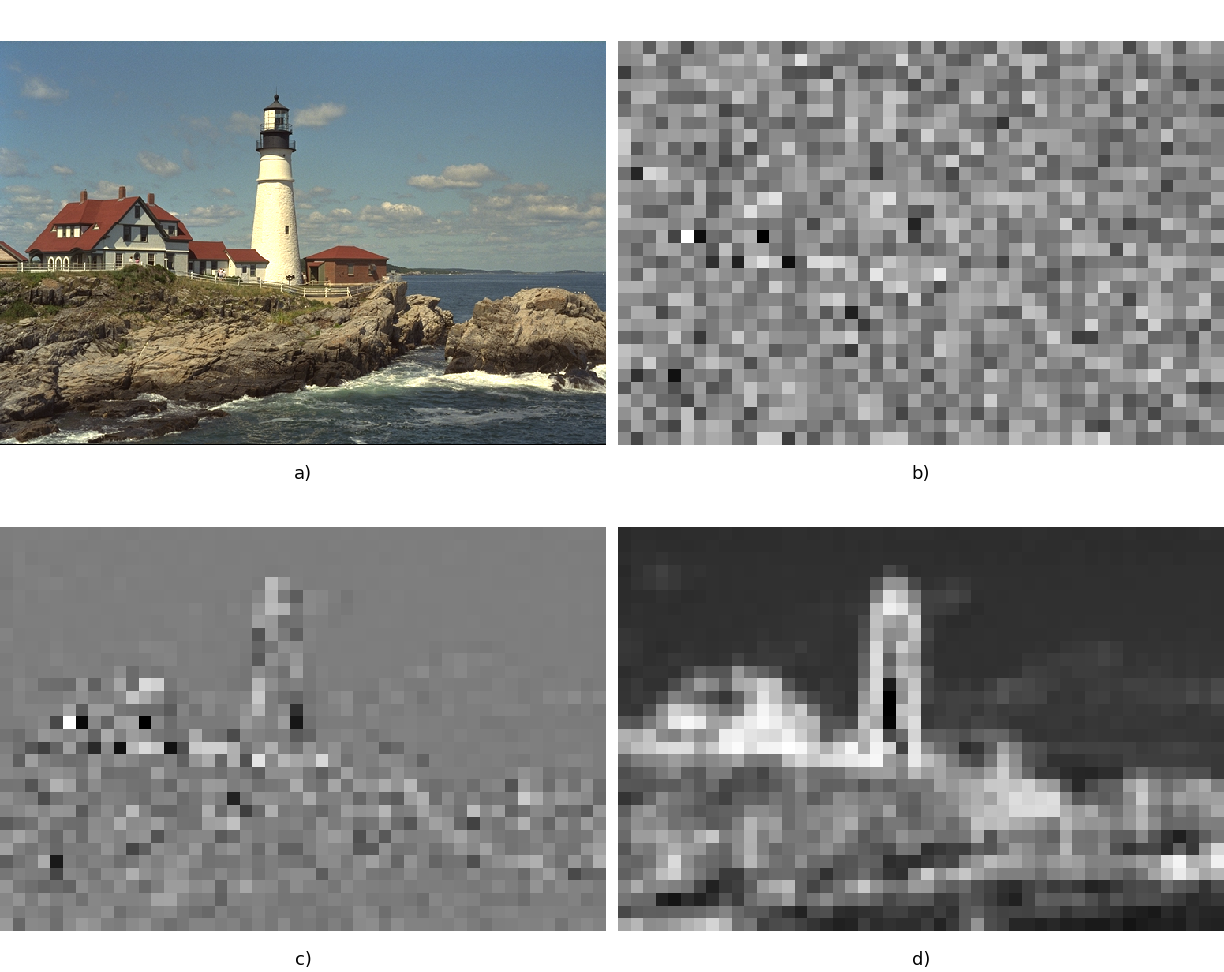
\includegraphics[width=\textwidth]{vae_rand_posterior.png}
  \caption[Latent spaces induced by \texttt{kodim21} in our VAE.]
  {\textbf{a)} \texttt{kodim21.png} from the Kodak Dataset. \textbf{b)}
    A random sample from the VAE posterior. \textbf{c)} Posterior means in a
  randomly selected channel. \textbf{d)} Posterior standard deviations in the same
  randomly selected channel. We can see that there is a lot of structure in the
  latent space, on which the full indepenence assumption will have a detrimental
  effect. (We have examined several random channels and observed the
  similarly high structure. We present the above cross-section without preference.)}
  \label{fig:vae_rand_posterior}
\end{figure}

\paragraph{}
In a regular VAE, we have a first level encoder, that given some input
$\vec{x}$ predicts the posterior
\[
  q^{(1)}(\vec{z}^{(1)} \mid \vec{x}) = \Norm{\vec{z}^{(1)} \mid
  \MU^{e, (1)}(\vec{x}), \SIGMA^{e, (1)}(\vec{x})},
\]
where $\MU^{e, (1)}(\vec{x}) = (m \circ f)(\vec{x})$ predicts the mean and
$\SIGMA^{e, (1)}(\vec{x}) = (\exp \circ s \circ f)(\vec{x})$ predicts the
standard deviation of the posterior. Here $f$ is a highly nonlinear mapping of
the input; in reality corresponding to several layers of neural network
layers. Notice that $f$ is shared for the two statistics. Then, $m$ and $s$ are
custom linear transformations, and finally we take the exponential of $s \circ f
$ to force the standard deviation to be positive. We sample $\tilde{\vec{z}}^{(1)}
\sim q^{(1)}$. We show a typical posterior distribuion given an image in Figure
\ref{fig:vae_rand_posterior}.
The first level prior is usually assumed to be a diagonal Gaussian
\[
  p^{(1)}(\vec{z}^{(1)})  = \Norm{\vec{z}^{(1)} \mid \vec{0}, I}.
\]
Finally, the first level decoder predicts the statistics of the data likelihood,
\[
  p(\vec{x} \mid \tilde{\vec{z}}^{(1)}).
\]

\paragraph{A note on the latent distributions} We have chosen to use Gaussian
latent distributions due to their simplicity, as well as their extenesibility to
PLNs (see Section \ref{sec:prob_ladder_networks}). On the other hand, we note
that Gaussians are inappropriate, as it has been shown that the filter responses
of natural images usually follow a heavy-tailed distribution, usually assumed to
be a Laplacian (\cite{jain1989fundamentals}), as used directly in
(\cite{clic2018winner}), but can also be approximated reasonably well by Gaussian
Scale Mixtures (\cite{portilla2003image}), as adopted by \cite{theis2017lossy}.
While it would be interesting to investigate incorporating these into our
model, as they do not extend trivially to our more complex model settings (in
particular PLNs, as we formulated them here requre the latent posterior
distribution's family to be self-conjugate), we leave this for future work.




\subsection{Data Likelihood and Training Objective}
\begin{figure}
  \centering
  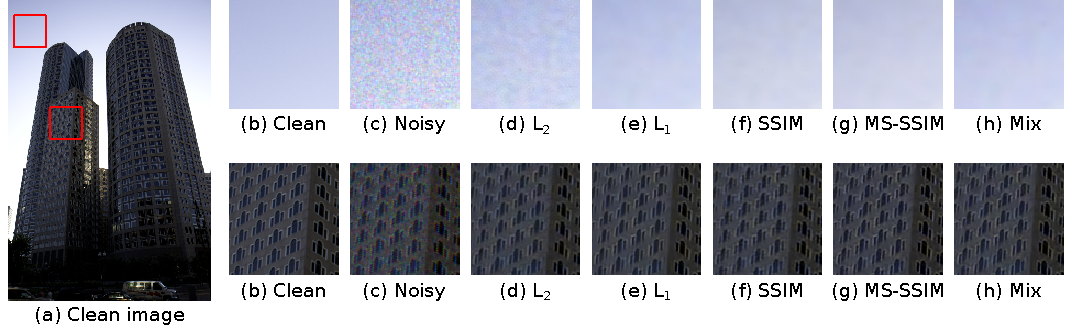
\includegraphics[width=\textwidth]{zhao_loss_comparison.pdf}
  \caption[Loss comparison for neural image reconstruction.]
  {Image reconstruction quality comparison on the task of joint
    image denoising and demosaicing, for the same architecture optimized using
    different distortion metrics. \textbf{a)-b)} Show the original image.
    \textbf{c)} Show the input to the networks. \textbf{d) - h)} Show
    reconstructions using various distrotion metrics. Mix is (approximately)
    defined as $(1 - \lambda) L_1 + \lambda \text{MS-SSIM}$ for $\lambda = 0.84$.
    The differences are best
    seen on the electronic version, zoomed in. We can clearly see the patchy
    artifacts introduced by Mean Squared Error (\textbf{d)}), and how much
    better Mean Absolute Error (\textbf{e)}) performs compared to it.
    (Image taken from \cite{zhao2015loss}. We changed the fonts of their
    captions to a sans-serif font for better readabitity.)}
  \label{fig:zhao_loss_comparison}
\end{figure}
\par
Based on the framework presented in Section
\ref{sec:compression_without_quantization}, the training objective used to train
the VAE is the (weighted) ELBO:
\begin{equation}
\label{eq:regular_vae_elbo}
\Exp{\log p(\vec{x} \mid \vec{z}^{(1)})}{q^{(1)}(\vec{z}^{(1)})}
- \beta \KL{q^{(1)}(\vec{z}^{(1)} \mid \vec{x})}{p^{(1)}(\vec{z}^{(1)})}.
\end{equation}
As the latent posterior and prior are both Gaussians, the KL can be computed
analytically, and there is no need for a Monte Carlo estimation. A popular and
simple choice for the likelihood to be chosen a Gaussian, in which case the
expectectation of the log-likelihood corresponds to the mean squared error
between the original image and its reconstruction. This also corresponds to
optimizing for the PSNR as the perceptual metric. However, PSNR correlates badly
with the HVS's perception of image quality (\cite{girod1993s}
\cite{eskicioglu1994image}). This is mainly because an MSE training objective is
tolerant to small deviations regardless of the structure in the image, and hence
this leads to blurry colour patch artifacts in low-textured regions, which the
HVS quickly picks up as unpleasant. A thorough survey of different
training losses for image reconstruction was performed by
\cite{zhao2015loss}, see Figure \ref{fig:zhao_loss_comparison}. Optimizing the
MS-SSIM distortion for the same architecture, they show that the artifacts are
greatly reduced. They also show that, somewhat surprisingly, Mean Absolute Error
(MAE) also significantly reduces and in some cases completely removes the
unpleasant artifacts introduced by MSE.
This is because MAE no longer underestimates small deviations, at the cost of
somewhat blurrier edges, which MSE penalized more. The MAE corresponds to a
diagonal Laplacian log-likelihood with unit scale, which is what we decided to
use in our experiments. This results in efficient training (an MS-SSIM
training loss, though differentiable, is very expensive to compute) as well as
it will enable us to use a further enchancement, see Section
\ref{sec:learn_gamma}.

Concretely, our likelihood is going to be
\begin{equation}
\label{eq:laplace_likelihood}
  p(\vec{x} \mid \vec{z}^{(1)}) = \Laplace{\hat{\vec{x}} \mid
  \MU^{d, (1)}(\tilde{\vec{z}}^{(1)}), I},
\end{equation}
where $\MU^{d, (1)}$ is the reverse operation of $\MU^{e, (1)}$.


\subsection{Probabilistic Ladder Network}
\label{sec:prob_ladder_networks}

\begin{figure}
  \centering
  \includegraphics[width=\textwidth]{VAE_architecture.png}
  \caption[Our Probabilistic Ladder Network (PLNl) architecture.]
  {PLN network architecture. The blocks signal data transformations, the
    arrows signal the flow of information. \textbf{Block descriptions:}
    \textit{Conv2D:} 2D convolutions along the spatial dimensions, where the
    $W\times H \times C / S$ implies a $W \times H$ convolution kernel, with $C$
  target channels and $S$ gives the downsampling rate (given a preceding letter
  ``d'') or the upsampling rate (given a preceding letter ``u''). If the slash
  is missing, it means that there is no up/downsampling. All convolutions operate
  in \texttt{same} mode with mirror padding. \textit{GDN / IGDN:} these are the
  non-linearities described in \cite{balle2016end}. \textit{Leaky ReLU:}
  elementwise non-linearity defined as $\max\{x, \alpha x\}$, where we set
  $\alpha=0.2$. \textit{Sigmoid:} Elementwise non-linearity defined as
  $\frac{1}{1 + \exp\{-x\}}$. We ran all
  experiments presented here with $N = 196, M = 128, F = 128, G = 24$.}
  \label{fig:pln_architecture}
\end{figure}

\par
We now introduce two extensions of VAEs to accomodate more complex latent
dependency structures: hierarchical VAEs (H-VAEs) and Probabilistic Ladder
Networks (PLNs) (\cite{sonderby2016train}). For simplicity's sake, we only
consider two-level H-VAEs and PLNs, the these can be easily extended to more
stochastic levels. In both cases, we essentially stack VAEs on top of each
other and train them together, though the way this is done is crucial for our
use case.

\par
To extend the VAE architecture from Section \ref{sec:method_vaes} to get a
2-level H-VAE, once $\tilde{\vec{z}}^{(1)}$ is sampled, we use it to predict
the statistics of the second level posterior
\[
  q^{(2)}(\vec{z}^{(2)} \mid \tilde{\vec{z}}^{(1)}) = \Norm{\vec{z}^{(2)} \mid 
  \MU^{e, (2)}(\tilde{\vec{z}}^{(1)}), \SIGMA^{e, (2)}(\tilde{\vec{z}}^{(1)})},
\]
where $\MU^{e, (2)}(\tilde{\vec{z}}^{(1)})$ and
$\SIGMA^{e, (2)}(\tilde{\vec{z}}^{(1)})$ are analogous to their first level
counterparts. Next the second level is sampled $\tilde{\vec{z}}^{(2)} \sim
q^{(2)}$. The second level prior $p^{(2)}(\vec{z}^{(2)})$ is now the diagonal
unit-variance Gaussian, and the first level priors' statistics are predicted
using $\tilde{\vec{z}}^{(2)}$:
\[
  p^{(1)}(\vec{z}^{(1)} \mid \tilde{\vec{z}}^{(2)}) =
  \Norm{\vec{z}^{(1)} \mid \MU^{d, (2)}(\tilde{\vec{z}}^{(2)}),
    \SIGMA^{e, (2)}(\tilde{\vec{z}}^{(2)})}.
\] 
The data likelihood's mean is predicted using $\tilde{\vec{z}}^{(1)}$ as before
(\cite{sonderby2016train}).
\par
The issue with H-VAEs is that the flow of information is limited by the
bottleneck of the final stochastic layer. PLNs resolve this issue by allowing
the flow of information between lower levels as well. To arrive at them, we
make the following modification to our H-VAE: first, once $q^{(1)}$ is known,
instead of sampling it immediately, we instead use its mean to predict the
statistics of the second level posterior:
\[
  q^{(2)}(\vec{z}^{(2)} \mid \tilde{\vec{z}}^{(1)}) = \Norm{\vec{z}^{(2)} \mid 
  \MU^{e, (2)}(\MU_{\vec{x}}), \SIGMA^{e, (2)}(\MU_{\vec{x}})},
\]
where $\MU_{\vec{x}} = \MU^{e, (1)}(\vec{x})$. Now, $\tilde{\vec{z}}^{(2)} \sim
q^{(2)}$ is sampled. The first level prior $p^{(1)}$ is calculated as before.
Finally, we allow the flow information on the first level by setting the
posterior $q^{(1)}$ as the combination of the statistics predicted on the first
level from the data and the statistics of $p^{(1)}$, inspired by the
self-conjugacy of the Normal distribution in Bayesian inference\footnotemark:
\[
  q^{(1)}(\tilde{\vec{z}}^{(1)} \mid \tilde{\vec{z}}^{2}, \vec{x}) =
  \Norm{\tilde{\vec{z}}^{(1)} \,\bigg|\,
    \frac{\SIGMA_{\vec{z}^{(1)}}^{-2} \MU_{\vec{x}} + \SIGMA_{\vec{x}}^{-2}
      \MU_{\vec{z}^{(1)}}}{\SIGMA_{\vec{x}}^{-2} + \SIGMA_{\vec{z}^{(1)}}^{-2}
    },
  \frac{1}{\sqrt{\SIGMA_{\vec{x}}^{-2} + \SIGMA_{\vec{z}^{(1)}}^{-2} }}},
\]
where $\MU_{\vec{x}} = \MU^{e, (1)}(\vec{x}), \MU_{\vec{z}^{(1)}} = \MU^{d, (2)}(\tilde{\vec{z}}^{(2)})$
and $\SIGMA_{\vec{x}} = \SIGMA^{e, (1)}(\vec{x}), \SIGMA_{\vec{z}^{(1)}} = \SIGMA^{d, (2)}(\tilde{\vec{z}}^{(2)})$.
We sample $\tilde{\vec{z}}^{(1)} \sim q^{(1)}(\tilde{\vec{z}}^{(1)} \mid
\tilde{\vec{z}}^{(2)}, \vec{x})$, and predict the mean of the likelihood using it.
\par 
The reason why H-VAEs and PLNs are more powerful models than regular VAEs, is
because regular VAEs make an independence assumption between the latents to make
the model tractable to compute, while H-VAEs and PLNs relax this to a
\textit{conditional indpendence} assumption. In this sense, the architecture of 
\cite{balle2018variational} also defines a PLN. We present the PLN architecture
we used in our experiments in Figure \ref{fig:pln_architecture}. We demonstarte
the power of the conditional independence in PLNs compared to the full independence
assumption in Figure \ref{fig:ladder_rand_posterior}.

\footnotetext{We note that the formula we used in our definition is the actual
  combination rule for a Gaussian likelihood and Gaussian prior. The formula given in
  \cite{sonderby2016train} is slightly different. We are not sure if it is a
  typo or it is what they actually used. We found our combination rule worked
  quite well in practice.}

\begin{figure}
  \centering
  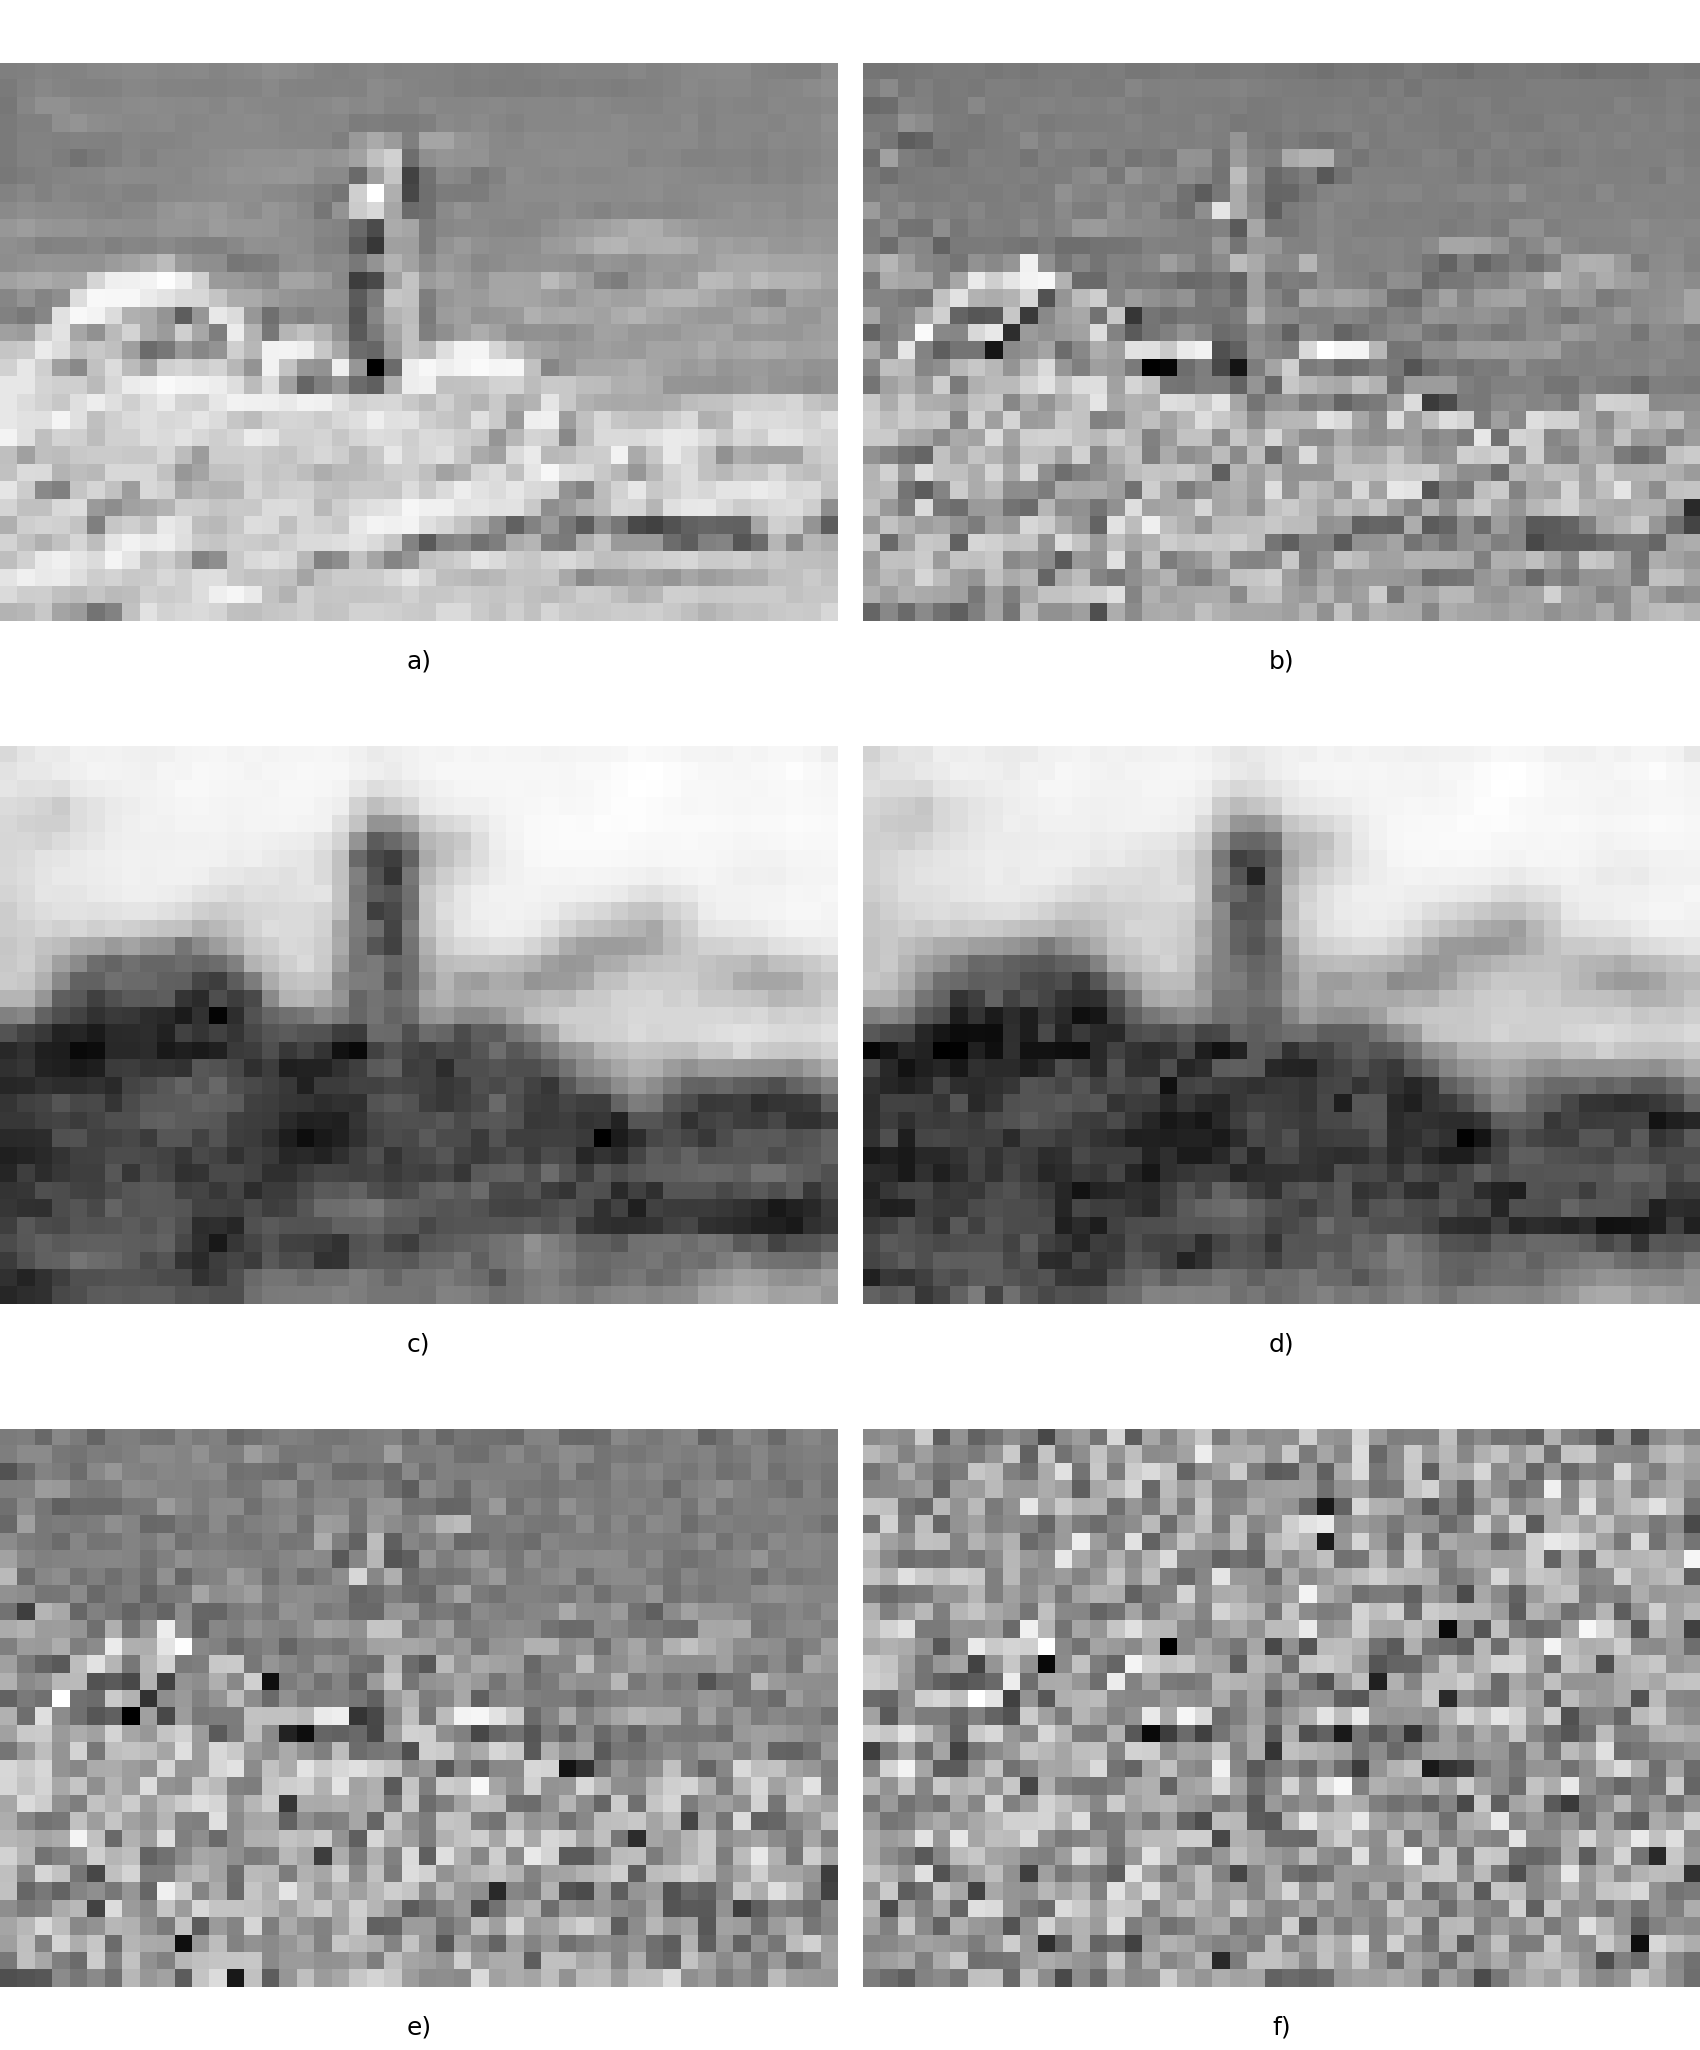
\includegraphics[width=\textwidth]{ladder_rand_posterior.png}
  \caption[Latent spaces induced by \texttt{kodim21} in our PLN]
  {We continue the analysis of the latent spaces induced by
    \texttt{kodim21} from the Kodak Dataset. Akin to Figure
    \ref{fig:vae_rand_posterior}, we have selected a random channel for both the
    first and second levels each and present the spatial cross-sections along these
    channels. \textbf{a)} Level 1 prior means. \textbf{b)} Level 1 posterior means.
    \textbf{c)} Level 1 prior standard deviations. \textbf{d)} Level 1 posterior
    standard deviations. \textbf{e)} Random sample from the Level 1 posterior.
    \textbf{f)} The sample from \textbf{e)} standardized according to the level
    1 prior. Most structure from the sample is removed, hence we see that the
    second level has successfully learned a lot of the dependencies between the
    latents. We have checked cross-sections along several randomly selected
    channels and observed the same phenomenon. We present the above with no preference.}
  \label{fig:ladder_rand_posterior}
\end{figure}

\paragraph{}
Finally we need to update the regularizing term of the ELBO to incorporate the
joint posterior and priors over the latents. This works out to be
\begin{align*}
  \KL{q(\vec{z}^{(1)}, \vec{z}^{(2)} \mid \vec{x})}{p(\vec{z}^{(1)}, \vec{z}^{(2)})} =\,\,& 
  \KL{q(\vec{z}^{(2)} \mid \vec{x})}{p(\vec{z}^{(2)})} + \\
  &\KL{q(\vec{z}^{(1)} \mid \vec{z}^{(2)} , \vec{x})}{p(\vec{z}^{(1)} \mid \vec{z}^{(2)})},
\end{align*}
which we can also compute analytically.

\section{Training}
\par \cite{sonderby2016train} give two key advices to train PLNs:
\begin{itemize}
\item Use batch normalization (BN) (\cite{ioffe2015batch}).
\item Use a warmup on the coefficient of the KL term in the loss.
  Concretely, given a target coefficient $\beta_0$, the actual coefficient they
  recommend should be
  \[
    \beta(t) = \min\left\{ \frac{t}{W}, 1 \right\} \times \beta_0,
  \]
  where $t$ is the current iteration and $W$ is the \textit{warmup period}.
\end{itemize} 
We ended up not utilizing point 1, due to an argument of
\cite{balle2018variational}, namely that GDN already performs a similar kind of
normalization as BN, and it did not improve their results. 

\subsection{Learning the Variance of the Likelihood}
\label{sec:learn_gamma}
\par
As we have noted, the reconstructions are blurry.
A solution offered by \cite{dai2019diagnosing} is to introduce a new parameter
$\gamma$ to the model, that will be the scale of the data likelihood. In our
case, since we are using a Laplace likelihood, we will have
\[
  p(\hat{\vec{x}} \mid \vec{z}^{(1)}) = \Laplace{\hat{\vec{x}} \mid \MU^{d,
      (1)}(\tilde{\vec{z}}^{(1)}), \gamma}.
\]
In the case of a Gaussian, $\gamma$ would be the variance of the distribution.
Then, it is suggested that instead of predicting gamma (i.e. using a
heteroscedastic model), or setting it as a hyperparameter, \textit{we learn it}.
In \cite{dai2019diagnosing} this is used in conjunction with another novel
technique to achieve generative results with VAEs that are competitive with
state-of-the-art GANs (\cite{goodfellow2014generative}). In this work, however,
as the second technique is irrelevant to us, we focus on learning $\gamma$ only.
\par
Let us examine this concept a bit more: let $D$ be the (original) log-likelihood
term with unit scale, and $R$ the (original) regularizing term, already
multiplied by our target coefficient $\beta$. Then, our new loss is going to be
\[
  L = \frac{1}{\gamma}D + R.
\]
Multiplying this through by $\gamma$ does not change the minimizer\footnotemark of the
expression, but we get the new loss
\[
  L' = D + \gamma R.
\]
\cite{dai2019diagnosing} show that if $\gamma$ is learned, then under some mild
assumptions $\gamma \rightarrow 0$ as $t \rightarrow \infty$ (where $t$ is the
number of iterations in the training procedure). This means that if we set some
target $\gamma_\infty$, and use
\[
  \gamma' = \max\{ \gamma, \gamma_\infty \},
\]
as the scale of the data likelihood, we actually get a dual effect to the warmup
recommended by \cite{sonderby2016train}, but with automatic scaling.
\footnotetext{\url{https://openreview.net/forum?id=B1e0X3C9tQ&noteId=ByeNgv9KTQ}}
\par
In parctice, $\gamma$ does not converge to 0, but to a number very close to
zero, which in experiments was around $\approx 0.02$, and hence instead of using
$\gamma'$, we set different $\beta$s to achieve different rate-distrotion
results. From now on, we will refer to PLNs where we also learned $\gamma$ as
$\gamma$-PLNs. In Figure \ref{fig:gamma_rand_posterior} we show the posterior of 
one of our $\gamma$-PLNs.
\begin{figure}
  \centering
  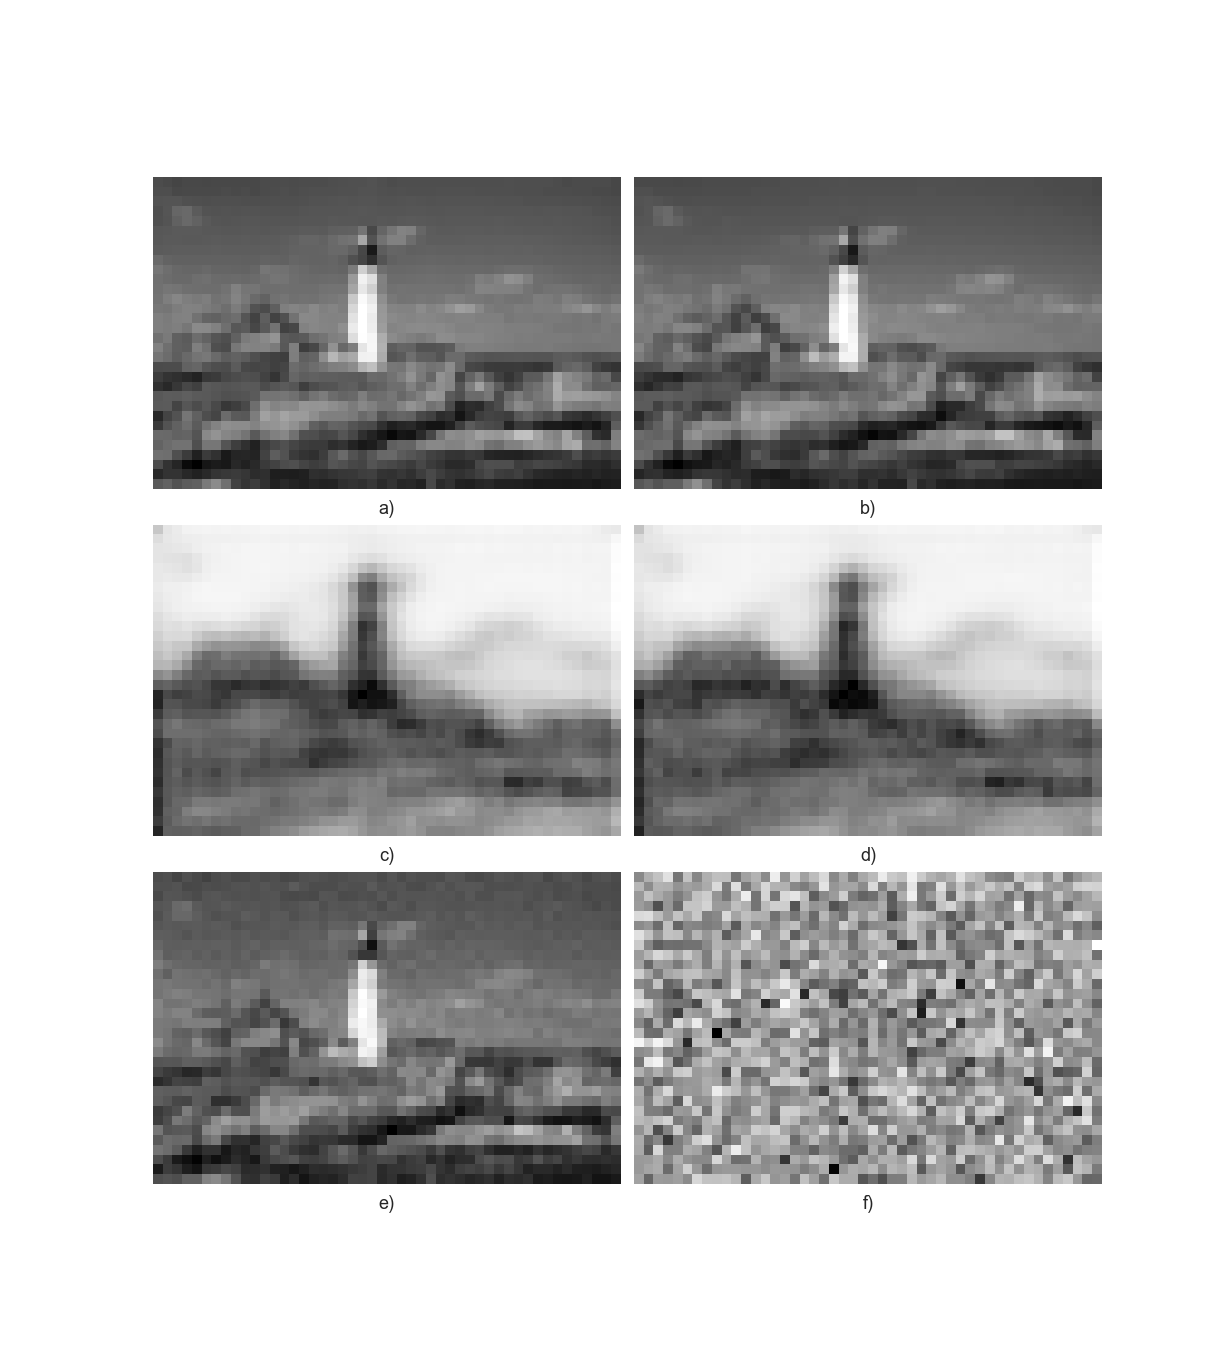
\includegraphics[width=\textwidth]{gamma_rand_posterior.png}
  \caption[Latent spaces induced by \texttt{kodim21} in our $\gamma$-PLN.]
  {We continue the analysis of the latent spaces induced by
    \texttt{kodim21} from the Kodak Dataset. Akin to Figures
    \ref{fig:vae_rand_posterior} and \ref{fig:ladder_rand_posterior},
    we have selected a random channel for both the
    first and second levels each and present the spatial cross-sections along these
    channels. \textbf{a)} Level 1 prior means. \textbf{b)} Level 1 posterior means.
    \textbf{c)} Level 1 prior standard deviations. \textbf{d)} Level 1 posterior
    standard deviations. \textbf{e)} Random sample from the Level 1 posterior.
    \textbf{f)} The sample from \textbf{e)} standardized according to the level
    1 prior. We observe the same phenomenon, with no significant difference, as
    in Figure \ref{fig:ladder_rand_posterior}. We note that while the posterior
    sample may seem like it has more significant structure than the one in the
    previous Figure. This is only coincidence; some of the regular PLN's
    channels contain similar structure, and some of the $\gamma$-PLN's channels
    contain more noisy elements.
  }
  \label{fig:gamma_rand_posterior}
\end{figure}

\section{Sampling and Coding}
\label{sec:coded_sampling}
\par
Once the appropriate network has been trained, this means that for any image $\vec{x}$
we are able to produce a latent posterior $q(\vec{z} \mid \vec{x})$ and prior
$p(\vec{z})$. The next step in our framework is to use a bits-back efficient coded sampling
algorithm to code a sample from the posterior. The first practical coded
sampling algorithm to was described in \cite{havasi2018minimal}, but there
are several key differences between our setting and theirs:

\begin{itemize}
\item \textbf{Variable sized latent space:} The original method was
  developed for compressing the weight distribution of a BNN, whose dimension is
  fixed. In our case, due to our fully convolutional architecture, our rendition
  of the algorithm must be able to adapt gracefully to a range of latent space
  dimensions. 

\item \textbf{Different posterior effects:} As our latent spaces will carry much
  more information about the topological nature of the coded image, the
  distribution of informative versus non-informative posteriors and their
  properties will be different from the original setting, and we will need to
  adapt to these effects. These effects can be clearly seen in Figures
  \ref{fig:vae_rand_posterior}, \ref{fig:ladder_rand_posterior} and
  \ref{fig:gamma_rand_posterior}.

\item \textbf{Practicality / Resource efficiency:} Since the original method has
  been proposed to compress neural networks after they have been trained, the
  algorithm was proposed with people who have sufficient resources to train them
  in mind. In particular, the original method incorporates several rounds of
  incremental retraining during the compression process to maintain low distortion, which
  might require several GPU hours to complete. As our aim in this work to
  present a practical, universal compression algorithm, we must also design our
  method with a much broader audience in mind. Though we still assume the
  presence of a GPU, our requirements and coding times are much lighter than
  that of the original work.
\end{itemize}

In the rest of this section we present the ways we addressed the above points.

\subsection{Parallelized Rejection Sampling and Arithmetic Coding}

\paragraph{Sampling}
As a baseline, we designed a parallelized version of Algorithm
\ref{alg:harsha_rej_sampling}, the original bits-back efficient sampling
algorithm presented by \cite{harsha2007communication}. As pointed out by
\cite{havasi2018minimal}, this algorithm quickly becomes intractable once
we leave the univariate setting. Fortunately, as we are working with
(conditional) independence assumptions between the latents, 
sampling each dimension individually and then concatenating them will also
give an exact multivariate sample.

\begin{algorithm}
  \caption{Parallelized, bit-budgeted rejection sampling based on Algorithm
    \ref{alg:harsha_rej_sampling}.}
  \label{alg:multivariate_rej_samp}
  \begin{algorithmic}
    \State \textbf{Inputs:}
    \State $B$ - Bit budget for coding the rejection sample indices
    \State $P$ - Prior probability mass function
    \State $Q$ - Posterior probability mass function
    \State $\langle x_i \sim Q \mid i \in \Nats \rangle$ - Sequence of random draws
    from $Q$
    \Statex
    \Procedure{Rej-Sampler}{$B, P, Q, \langle x_i \sim Q \mid i \in \Nats \rangle$}
    \State $D \gets \text{dim}(P)$
    \State $p_{d, 0}(x) \gets 0 \quad \forall x \in \X, \forall d = 1,\hdots D$.
    \State $p_{d, 0}^* \gets 0, \forall d = 1,\hdots D$.
    \State $A = \vec{0} \in \{0, 1\}^D$
    \Comment Keeps track of whether a dimension has been accepted or not

    \State $S = \vec{0} \in \Reals^D$
    \Comment Sample we are ``building''

    \State $I = -\vec{1} \in \Nats^D$
    \Comment Index vector for each dimension

    \For{$i \gets 1, \hdots 2^B$}

    \For{$d \gets 1, \hdots D$}

    \If{$A_d = 1$}

    \State Skip

    \EndIf


    \State
    $\alpha_{d, i}(x) \gets \min{P_d(x) - p_{d, i - 1}(x), (1 - p_{d, i - 1}^*)Q_d(x)}\quad
    \forall x \in \X$

    \State $p_{d, i}(x) \gets p_{d, i - 1}(x) + \alpha_{d, i}(x)$
    
    \State $p_{d, i}^* \gets \sum_{x \in \X}p_{d, i}(x)$

    \State $\beta_{d, i}(x_i) \gets \frac{\alpha_{d, i}(x)}{(1 - p_{d, i}^*)Q_d(x)}$

    \State Draw $u \sim \Unif{0, 1}$

    \If{$u < \beta_{d, i}(x_i)$}

    \State $A_d \gets 1$
    \Comment Indicate we accepted the sample

    \State $S_d \gets x_i$
    \State $I_d \gets i$

    \EndIf
    
    \EndFor
    \EndFor

    \State Draw $S' \sim Q_{\text{where } I = -1}$
    \Comment Sample dimensions where we have not accepted.

    \State $S_{\text{where } I = -1} \gets S'$
    \Comment Set the ``built'' sample's missing dimensions to $S'$.

    \State $I_{\text{where } I = -1} \gets $ \Call{Quantize}{$S', 16$}
    \Statex
    \Comment Set the missing dims. of $I$ to $S'$ quantized to 16 bits. 

    \State\Return $I, S$
    \EndProcedure
  \end{algorithmic}
\end{algorithm}

\par
We modify Algorithm \ref{alg:harsha_rej_sampling} in two ways to make it more
efficient. While their algorithm is Las Vegas, i.e. it always gives the right
answer, but in random time, this can get very inefficient if we have a few
dimensions with very high KL divergence. We circumvent this issue and fix the
runtime of the algorithm by allocating a bit budget $B$ to each dimension, and
only allowing $2^B$ samples to be examined. If the sample is accepted within
these draws, then we have a code for them. The dimensions where all $2^B$ samples were
rejected, we sample from the target $q$, and quantize the samples to 16 bits.
This gave about a 1\% increase in size at a much imporved runtime. In
particular, for dimensions with KL larger than 16 bits this is actually more
efficient than coding them with Algorithm \ref{alg:harsha_rej_sampling}.
We then use the quantized samples as code. The concrete details can be seen in Algorithm
\ref{alg:multivariate_rej_samp}. Instead of using the density of the posterior
and the prior to sample, we finely quantized them and used the probability
masses in the algorithm.

% why doesnt rejection sampling work exactly?
% - the cost is not arising from bad independence assumptions, because we have
%   indepenedence
% - so does it come from a bad match of the actual image posteriors?

\paragraph{Coding}
Simply writing the codes of the individual dimensions given by the rejection
sampler would be very inefficient, because without additional assumptions the
way to uniquely decode them would be to block code them (i.e. code all indices
in 8 bits, say). This would however would add an $\Oh(1)$ cost per dimension on
the coding length, which is very undesirable. Hence, we implemented a simple
non-adaptive arithmetic coder (\cite{rissanen1981universal}) to mitigate this issue.
Probabilities for the symbol table have been estimated by encoding the entire
CLIC training set and using the empirical probability distribution on the
indices. We used Laplace/additive smoothing for unseen indices (\cite{chen1999empirical}).
In particular, given the empirical distribution of the sample indices $P$,
the probability distribution used is
\[
  \tilde{P}(i) = \begin{cases}
    (1 - \alpha)P(i) & \text{if } i \in I \\
    \frac{\alpha}{N} & \text{otherwise}
    \end{cases}
\]
where $I = \{i \in \Nats \mid P(i) > 0\}$.
In our case we allocated $B = 8$ bits for each individual dimension,
$I = \{0, \hdots 255\}$ as all codable indices appeared. Since we quantized the
outliers to 16 bits, $N = 2^{16} - 2^{8}$. We found that choosing $\alpha
\approx 0.01$ gave the best results.

\paragraph{A note on the Arithmetic Coder}
\par
While for small alphabets the naive implementation of the arithmetic coder is
very fast, the decoding time actually grows as $\Oh(|\A|)$ in the size of the
alphabet. In particular, decoding the arithmetic code of a reasonably large
image would take up to 30 minutes using the naive implementation on a CPU. The
inefficiency is due to a bottleneck where we need to find in a partition of $[0,
1]$ into which the currently coded interval fits. The naive
uses a linear search over the partitions. This can be made more efficient by
using height-balanced binary search trees (BSTs). In particular, we need to find
the least upper bounding item in the BST for the given point, which can be done
in $\Oh(\log_2|\A|)$ time.
Using this additional trick, we can decode large images' code in a few seconds.
In particular we implemented an AVL-tree to serve as the BST, which is always
guaranteed to be height balanced (\cite{adel1962algorithm}).

\paragraph{Issues} Theorem \ref{thm:bits-back_efficiency} guarantees that the
MDL of a realization of a random variable $Y$ given $X$ by using Algorithm
\ref{alg:harsha_rej_sampling} is
\[
  L(X) \leq \KL{q(Y \mid X)}{p(Y)} + 2\log\left( \KL{q(Y \mid X)}{p(Y)} + 1
  \right) + c,
\]
for some small constant $c$.
However, to achieve this for the joint latents $\vec{z}$, we would need to
sample them jointly, which is intractable. Instead, we sample the
dimensions individually, which by the same theorem introduces a $D\cdot c$ nat
extra length to the code, where we assumed $\vec{z} \in \Reals^D$. This is
because the constant cost $c$ is now incurred in every dimension. Since in our
case $D$ is usually on the magintudes of $10^5 - 10^6$ even for small $c$ this
cost becomes non-negligible. In our experiments (not show here) this lead to coding
efficiencies $2.5 - 3.5$ times worse than the optimal efficiency predicted by Theorem
\ref{thm:bits-back_efficiency} for the whole multivariate sample. This lead us
to abandon rejection sampling early on in the project for more efficient approximate methods,
which we describe below.

\subsection{Greedy Coded Sampling}
\begin{algorithm}
  \caption{Greedy Coded Sampler}
  \label{alg:greedy_sampler}
  \begin{algorithmic}
    \State \textbf{Inputs:}
    \State $K$ - Number of proposal shards
    \State $B$ - Bit budget for coding the seed of individual shards. 
    \State Will result in $2^B$ samples to be examined per shard.
    \State $\MU_p$ - Mean of proposal distribution
    \State $\SIGMA_p^2$ - Variance of proposal distribution
    \State $q$ - Posterior distribution
    \Statex
    \Procedure{Greedy-Sampler}{$K, B, \MU_p, \SIGMA_p^2, q$}

    \State $\tilde{\vec{z}}_0 \gets \vec{0}$
    \Comment Initialize the sample

    \State $I = ()$
    \Comment Initialize the index set to an empty list
    \For{$k = 1, \hdots, K$}

    \State Set random seed of generator to $k$.
    
    \State Draw $\vec{s}_{k, b} \sim \Norm{\frac{\MU_p}{K}, \frac{\SIGMA_p}{K}}
    \quad$ for $b = 1,\hdots,B$
    
    \State $\vec{c}_{k, b} = \tilde{\vec{z}}_{k - 1} + \vec{s}_{k, b}$

    \State $\tilde{\vec{z}}_k \gets \argmax_{\vec{c}_{k, b}} \left\{ \log q(\vec{c}_{k, b}) \right\}$
    \Comment Create new sample

    \State $i_k \gets \argmax_{b} \left\{ \log q(\vec{c}_{k, b}) \right\}$
    \Comment Store the index of the shard sample that we used

    \State Append $i_k$ to $I$.
    
    \EndFor

    \State \Return $\tilde{\vec{z}}_K, I$
    
    \EndProcedure
  \end{algorithmic}
\end{algorithm}
\par
To solve the issue of dimensionality, we need a way to code a sample
drawn from the multivariate distribution. The strategy of the greedy sampler is
to progressively ``build'' a reasonable sample from the posterior. A well
known fact about Gaussian distributed random variables is that they are
closed under addition. Concretely,
if $X \sim \Norm{\mu_X, \sigma^2_X}, Y \sim \Norm{\mu_Y, \sigma^2_Y}$, then
\[
  X + Y \sim \Norm{\mu_X + \mu_Y, \sigma_X^2 + \sigma_Y^2}.
\]
In the multivariate case assuming they are diagonal, the extension of
the above is straight forward.
Using this, we may now do the following: pick an integer $K$, that
we will call the \textit{number of shards}. Then, given the prior
$p(\vec{z} \mid \MU, \SIGMA^2)$, we can break it up into $K$ equal
shards $p_k\left(\vec{z} \mid \frac{\MU}{K}, \frac{\SIGMA^2}{K}\right)$.
Note, if we assign a different, but preagreed sequence of random seeds to each
shard, then each shard sample can be coded in $B$ bits that we can set. Start
with an initial sample $\tilde{\vec{z}}_0 = \vec{0}$ and draw $2^B$
samples $\vec{s}_{1, b}$ from the first shard $p_1$ and create
``candidate samples'' $\vec{c}_{1, b} =
\tilde{\vec{z}}_0 + \vec{s}_{1, b}$ and calculate their log-likelihoods under the
target. Finally, set $\tilde{\vec{z}}_1 = \argmax_{\vec{c}_{1, b}}\log
q(\vec{c}_{1, b})$, and repeat until we reach $\tilde{\vec{z}}_K$, at which
point we return it. Then the returned vector will be approximately from the
target. More precisely, this is a ``guided'' random walk, where we bias the
trajectory towards the median of the distribution. The code of the distribution
is then the codes of the selected shard samples, concatenated. The algorithm is described in
more detail in Algorithm \ref{alg:greedy_sampler}. 

\paragraph{A note on implementation}
We note that empirically the greedy sampler underperforms when the variances of the
some priors is small. To ameliorate this, we standardize the prior, and scale the
posterior according to the standardization, i.e. we set 
\[
  q'(\vec{z} \mid \vec{x}) = \Norm{\vec{z} \bigg| \frac{\mu_q -
      \mu_p}{\sigma_p}, \frac{\sigma^2_{q}}{\sigma^2_{p}}},
\]
where $\mu_p, \sigma^2_p$ are the statistics of the original prior and $\mu_q,
\sigma^2_q$ are the statistics of the original posterior. We communicate the
approximate sample $\vec{z}'$ from $q'$ instead of $q$. This is not problematic, as
Gaussian distributed random variables are closed under linear transformations,
i.e. given $X \sim \Norm{m, s^2}$, we have
\[
  \alpha X + \beta = Y \sim \Norm{\alpha m + \beta, \alpha^2 s^2}.
\]
Hence, the decoder may recover an approximate sample from $q$, by calculating
$\vec{z} = \sigma_{p} \vec{z}' + \mu_{p}$.
\paragraph{Issues}
While the greedy sampler makes sampling efficient and tractable from the
posterior, it comes at the cost of reduced sample quality. In particular, it
gives blurrier images. This also means that if we use a PLN to compress an
image and we use the greedy technique to code the latents on the second level,
the first level priors' statistics derived from the biased sample will be off,
and $\KL{q(\vec{z}^{(1)} \mid \tilde{\vec{z}}^{(2)}, \vec{x})}{p(\vec{z}^{(1)} \mid
  \tilde{\vec{z}}^{(2)})}$ will be higher. We have verified empirically, that while
using a biased sample on the second level does not degrade image quality
(possibly due to the noise tolerance of PLNs), it does significantly increase
the compression size (by a factor of $1.2 - 1.5$) of the first level, which is
very significant. This motivated the final sampling algorithm presented here,
only used on the second level of our PLNs.

\subsection{Adaptive Importance Sampling}
\begin{algorithm}
  \caption{Adaptive Importance Sampler based on Algorithm
    \ref{alg:miracle_imp_samp}, introduced by \cite{havasi2018minimal}}
  \label{alg:adaptive_importance_sampler}
  \begin{algorithmic}
    \State \textbf{Inputs:}
    \State $K$ - Maximum individual KL allowed
    \State $G$ - Maximum group size
    \State $B$ - Bit budget per group
    \State $P$ - Proposal distribution
    \State $Q$ - Target Distribution
    \State $\langle x_i \sim Q \mid i \in \Nats \rangle$ - Shared sequence of
    random draws from $Q$
    \Statex
    \Procedure{Adaptive-Importance-Sampler}{$K, G, B, P, Q, \langle x_i \sim Q \mid i \in \Nats \rangle$}
    \State $\Gamma \gets ()$
    \Comment Group sizes
    \State $kl_i \gets \KL{Q_i}{P_i} \forall i = 1, \hdots N$
    \Comment Get KLs for each dimension
    \State $OI \gets $ \Call{Where}{$kl_i > K$}
    \Comment Outlier indices in the vector
    \State Sample $O \sim Q_{OI}$
    \State $\hat{O} \gets $ \Call{Quantize}{O}
    \State $Q' \gets Q_{\setminus OI}$
    \Comment Target distribution restricted to the dimensions defined by $OI$.
    \State $P' \gets P_{\setminus OI}$
    \Comment Remove outlier dimensions
    \State $\gamma \gets 0$
    \Comment Current group size
    \State $k \gets 0$
    \Comment Current group KL

    \For{$i \gets 1, \hdots \text{dim}(Q')$}

    \If{$k + kl_i > B$ or $\gamma + 1> G$}

    \State Append $\gamma$ to $\Gamma$
    \State $k \gets kl_i$
    \State $\gamma \gets 1$

    \Else

    \State $k \gets k + kl_i$
    \State $\gamma \gets \gamma + 1$

    \EndIf

    \EndFor

    \State Append $\gamma$ to $\Gamma$
    \Comment Append the last group size

    \State $S = ()$
    \Comment Importance samples for the groups
    \State $I = ()$
    \Comment MIRACLE sample indices
    \State $g \gets 0$
    \Comment Current group index

    \For{$\gamma$ in $\Gamma$}
    \Comment Now importance sample each group

    \State $idx, s \gets$ \Call{Importance-Sample}{$P_{g:g + \gamma}, Q_{g: g +
        \gamma}, \langle x_i \sim Q \mid i \in \Nats \rangle$}
    \State Append $idx$ to $I$
    \State Append $s$ to $S$

    \EndFor

    \State \Return I, S

    \EndProcedure
  \end{algorithmic}
\end{algorithm}
The adaptive importance sampler uses the importance sampler described in
Algorithm \ref{alg:miracle_imp_samp}, introduced by \cite{havasi2018minimal}.
The idea is to use similar block-based importance sampling as proposed in
\cite{havasi2018minimal}. However, unlike them, we allocate the block sizes
dynamically. In particular, we set a bit budget $B$ per group, a maximum group
size $G$ and an individual limit $K$.
We begin by discarding individual dimensions where the KL is larger
than $K$. Then, we flatten the remaining dimensions in raster-scan order and 
iteratively add dimensions into the current group so long as the total KL of the
group reaches either the bit budget $B$ or the number of dimensions added to the
group reaches $G$. At this point we start with a new group. Once the whole
vector has been partitioned, we importance sample each group using Algorithm 
\ref{alg:miracle_imp_samp}. The removed dimensions are sampled directly from
the posterior and then the samples are quantized to 16 bits. The complete
algorithm can be seen in Algorithm \ref{alg:adaptive_importance_sampler}.
\par
For ease of referral, since we would perform Adaptive Importance Sampling on the
second level, followed by the Greedy Sampling on the first, We will refer to
this way of sample coding as IS-GS.

\paragraph{}
For the importance sampler, the $\Oh(1)$ sampling cost impeding the rejection
sampler is negligible, as it will be now shared across approximately $G$
dimensions. We can also forgo the arithmetic coder, as the indices output by the
sampler are already going to be quite efficient. On the other hand, we also
have to communicate the groups as well. Instead of communicating
group indices, we can instead order the latents and communicate consecutive
group sizes, from which the indices can be easily reconstructed. Each
group's size takes up at most $\lceil \log_2G \rceil$ bits. In total, we usually
get slightly more than $\left\lceil \frac{N_2}{G} \right\rceil$ groups,
(where $N_2$ is the dimensionality of the second level). This is still
very inefficient, but so long as $N_2$ is sufficiently small compared to the
codelength for the indices, it will be manageable. We also note that the group
size is likely to be biased towards higher values, and hence building an
empyrical distribution them and arithmetic coding the sequence could lead to a
big reduction in the inefficiency, however, we found this not to be too
important to focus on. 

\paragraph{Greedy Sampler} It is easy to see that the greedy sampler is already
as efficient as it could be. The sample indices for each shard are as compactly
represented, as we expect the maximum of the samples to be uniformly
distributed. Hence, the only other things that needs to be coded is the number
of shards and the number of samples for each shard for the cumulative sample to
be decodable. Hence, for the greedy sampler we just wrote the indices straight
to the binary file.

%!TEX root = ../thesis.tex
%*******************************************************************************
%****************************** Second Chapter *********************************
%*******************************************************************************

\chapter{Experiments}
\label{chapter:experiments}

\graphicspath{{../img/plots/vae_latents/}{../img/plots/kodak_comparison/}{../img/plots/kodak_coding_time/}{../img/plots/kodak_side_info/}{../img/plots/reconstructions/}}

\label{sec:experimental_results}
\par
In this chapter we detail our experimtal setup and empirically show the
correctness and the efficiency of our model. We compare our results to
two classical lossy image compression methods, JPEG, and BPG. JPEG is the most
widely used lossy compression method (\cite{bull2014communicating}), and hence
showing that we can outperform it is important to show the viability of our
method. BPG (Better Portable Graphics) is a more modern transform coding method,
that adapts to the statistics of images and is the current state-of-the-art in
classical lossy image compression (\cite{rippel2017real}).
We also compare to the current state-of-the-art in neural compression, the results of
\cite{balle2018variational}\footnotemark. We implemented all of our
architectures and experiments from scratch in \texttt{Python 3.5}, using \texttt{Tensorflow}
(\cite{tensorflow2015-whitepaper}) and \texttt{Sonnet} (\cite{sonnetblog})
libraries. All of our code is available publicly at
\url{https://github.com/gergely-flamich/miracle-compression}. 

\footnotetext{We thank the authors of the paper for making their data available
  to us.}

\section{Experimental Setup}
\par
As we based our models on the work of \cite{balle2016end} and
\cite{balle2018variational}, we mirror a lot of their training setup as well
(see Section \ref{sec:dataset_preproc} for the dataset and preprocessing). We
trained all our models with Adam (\cite{kingma2014adam}) with a starting
learning rate of $\alpha_0 =
3 \times 10^{-5}$ and trained all of our models for 20 epochs or equivalently,
approximately 200,000 iterations, by using batches of 8 image patches per
iteration. For training VAEs and regular PLNs, we used a smooth
exponential learning rate decay schedule according to the formula
\[
  \alpha(t) = \alpha_0 \times r^{\frac{t}{D}}.
\]
Where $r$ is the decay rate, $D$ is the decay step size and $t$ is the current
iteration. We found $r = 0.96$ and $D = 1500$ worked well for our
experiments. While we did not notice significant performance gains using the
learning rate scheduling, our models converged slighly faster.
\par
For $\gamma$-PLNs we found learning rate decay actually hurt the training
performance of the model, as it kept $\gamma$ from converging to 0.
\par
The architecture used for the VAE is the same as what we used for PLNs (shown in
Figure \ref{fig:pln_architecture}), with the second level omitted. For the
convolution capacities, we used $N = 192$ channels on the first
level and $M = 128$ channels on the second. We have significantly reduced the
channels on the latent dimensions compared to \cite{balle2018variational}, as we
use $F = 128$ and $G = 24$, where they use $F_{\text{Ball\'e}} = 192 / 320$, and
$G_{\text{Ball\'e}} = 128$. On the first level, we found that adding more
channels did not significantly increase the performance of our model, which we
credit to the more flexible latent distributions used in our model. On the other
hand, we chose $G = 24$ because we found that when increased beyond this, the
cost of communicating the group indices for the importance sampler became very
inefficient. With 24 channels, the overhead is already 30-40\% of the second
level's code length.
\par
In all experiments we used the adaptive importance sampler on the second level, and the
greedy sampler (IS-GS) on the first. For the importance sampler we used $K = 12$
bits as the outlier KL limit, $B = 20$ bits for the maximum total group KL and
$G = 16$ as the maximum number of dimensions in a single group. For the greedy
sampler we set $K = 30$ shards and $B = 14$ bits per shard, leading to $2^{14}$
samples per shard. See Section \ref{sec:coded_sampling} for a review of these terms.

\paragraph{}
All experiments were run on a GeForce GTX 1080 GPU.

\section{Results}
\begin{figure}
  \centering
  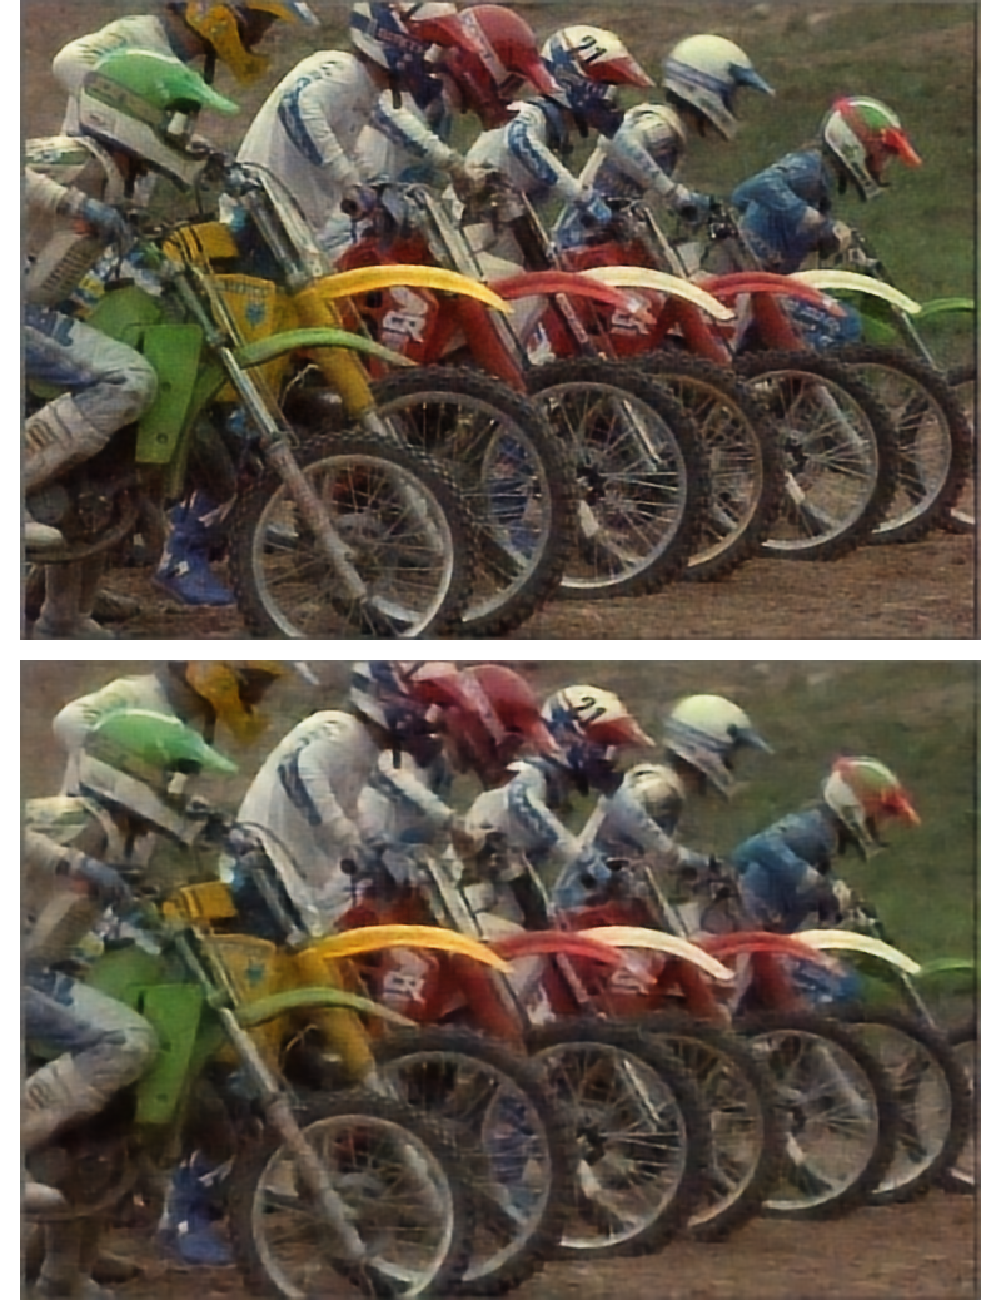
\includegraphics[width=\textwidth]{pln_003_01_k05.png}
  \caption[PLN reconstructions of \texttt{kodim05}.]
  {PLN reconstructions of \texttt{kodim05}. \textbf{Top:} $\beta =
    0.03$, 0.810 bpp, MS-SSIM: $0.913$, PSNR: $23.053$ dB \textbf{Bottom:}
    $\beta = 0.1$, 0.354 bpp, MS-SSIM: $0.848$, PSNR: $21.495$ dB.}
  \label{fig:pln_reconstruction}
\end{figure}
\begin{figure}
  \centering
  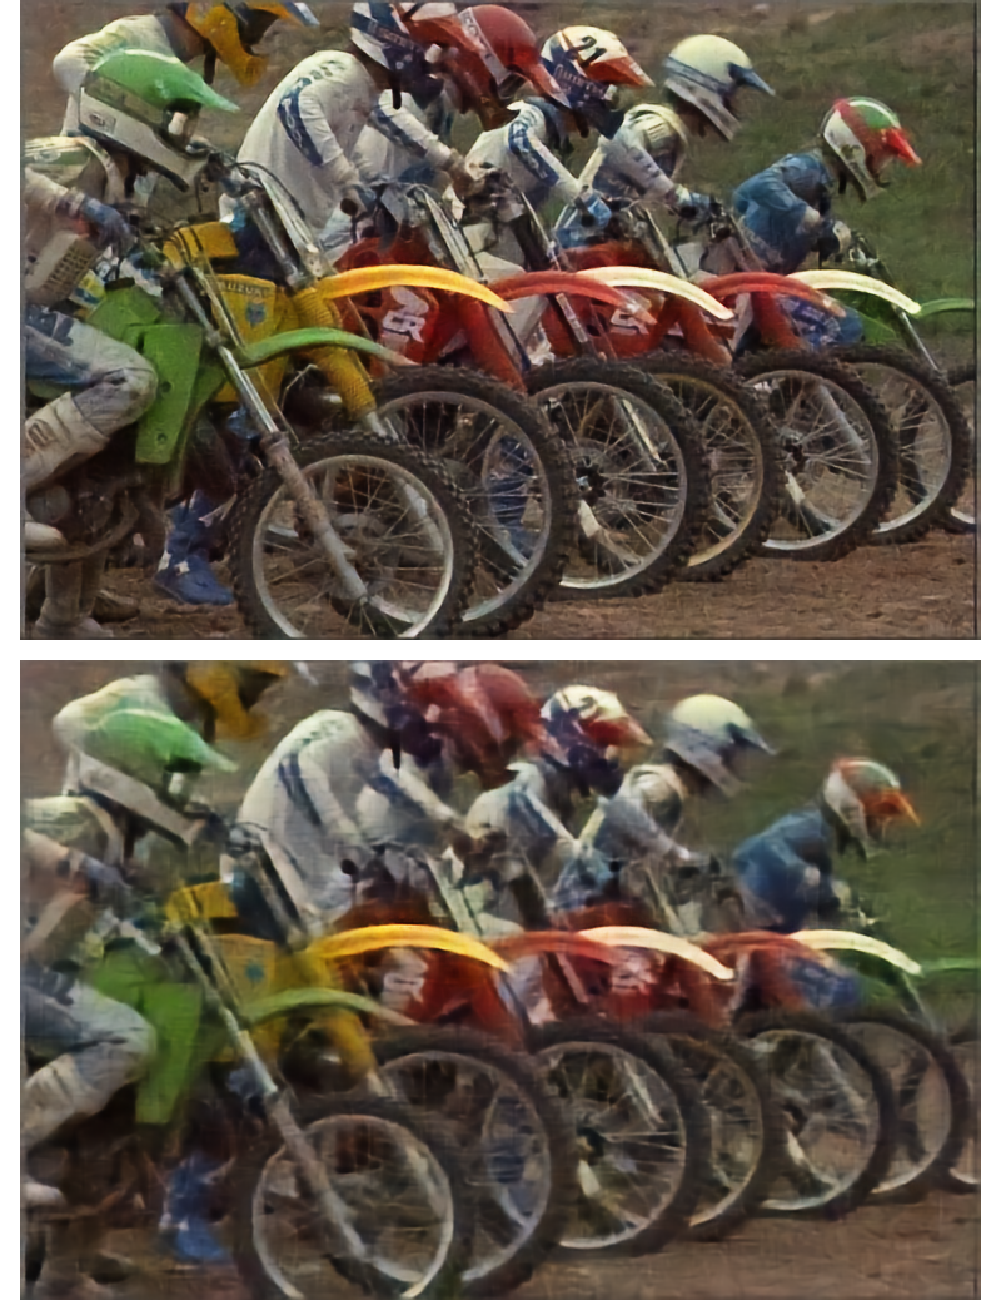
\includegraphics[width=\textwidth]{log_gamma_3_10_k05.png}
  \caption[$\gamma$-PLN reconstructions of \texttt{kodim05}.]
  {$\gamma$-PLN reconstructions of \texttt{kodim05}. \textbf{Top:}
    $\beta = 3$, 0.354 bpp, MS-SSIM: $0.937$, PSNR: $21.397$ dB \textbf{Bottom:}
    $\beta = 10$, 0.189 bpp, MS-SSIM: $0.824$, PSNR: $21.068$ dB.}
  \label{fig:gamma_reconstruction}
\end{figure}
\par

We present the rate-distorsion curves for the following:
\begin{itemize}
\item JPEG, with quality settings from 1 to 92, with increments of 7 between
  settings. As this is the most widely used lossy image compression codec
  (\cite{bull2014communicating}), it is
  crucial to demonstrate that our method is at least competitive with it, and
  ideally beats it.
\item BPG\footnotemark with 4:4:4 chroma sampling, as we are comparing against
  RGB-based compression techniques. We used quantization settings between 51 to
  33 with decrements of 3 between settings.
\item Two models with the same architecture from \cite{balle2018variational},
  one optimized for a MSE training objective, and one optimized for the
  MS-SSIM perceptual metric.
\item Two of our models, all of which were optimized with Laplacian likelihoods,
  one PLN and one $\gamma$-PLN. We trained the PLNs using $\beta =
  \{1, 0.3, 0.1, 0.03\}$ and the $\gamma$-PLNs using $\beta =
  \{10, 3, 1, 0.3, 0.1\}$. We plot both their theoretically optimal
  performance as well as their actual performance, with the differences
  explained below. The reason for not presenting results of the VAEs, is because
  their rate-distrotion curves are quite a lot worse than the other
  models', and would have distorted the figures too much.
\end{itemize}

\par
When presenting our method, for each model we present two results: the \textit{theoretically
optimal} performance, and the \textit{actual} performance. The theoretically
optimal bits per pixel (BPP) was calculated using the theoretically
achievable upper bound for the compression size in bits as given by
Theorem \ref{thm:bits-back_efficiency}, without the constant term. Concretely,
for a drawn latent sample $\tilde{\vec{z}}$ for image $\vec{x}$, it is 
\[
  \KL{q_\phi(\vec{x} \mid \tilde{\vec{z}})}{p_\theta(\tilde{\vec{z}})}
  + 2 \log \left( \KL{q_\phi(\vec{x}
      \mid \tilde{\vec{z}})}{p_\theta(\tilde{\vec{z}})} + 1 \right).
\]
The optimal reconstruction error was calculated by passing an image through the
PLN using a normal forward pass, instead of using the IS-GS approximate sample. Thus, any
actual method's performance using the same setup should appear to the right of
(worse rate) or below (worse distrotion) the theoretical position.

\footnotetext{We used the implementation available at \url{http://bellard.org/bpg}}

\par
We show a comparison between reconstructions at different rates of
\texttt{kodim05} from the Kodak Dataset (\cite{kodakdataset}) for PLNs in Figure
\ref{fig:pln_reconstruction} and for $\gamma$-PLNs in Figure
\ref{fig:gamma_reconstruction}. A much more thorough comparison of
reconstructions is given at the end of the thesis in Appendix \ref{chapter:appendix_b}.
\par
The rate-distortion curves for \texttt{kodim05} are shown in Figure
\ref{fig:kodim05_comp}. We observe a similar phenomenon as
\cite{balle2018variational}: there is a mismatch in the comparison
of models according to different perceptual metrics, depending on what objective
they have been optimized for. In particular, JPEG and BPG have both been
optimized so that they give high PSNR (thus, low MSE), whereas they underperform
on the newer MS-SSIM metric. MS-SSIM correlates better with how
the human visual system (HVS) perceives quality (\cite{msssim}),
hence it is generally more desirable to perform well on that metric
(\cite{toderici2017full}, \cite{rippel2017real}, \cite{balle2018variational}).
The fact that our models perform well on MS-SSIM also justifies our choice of
the MAE as the training objective.
\begin{figure}
  \centering
  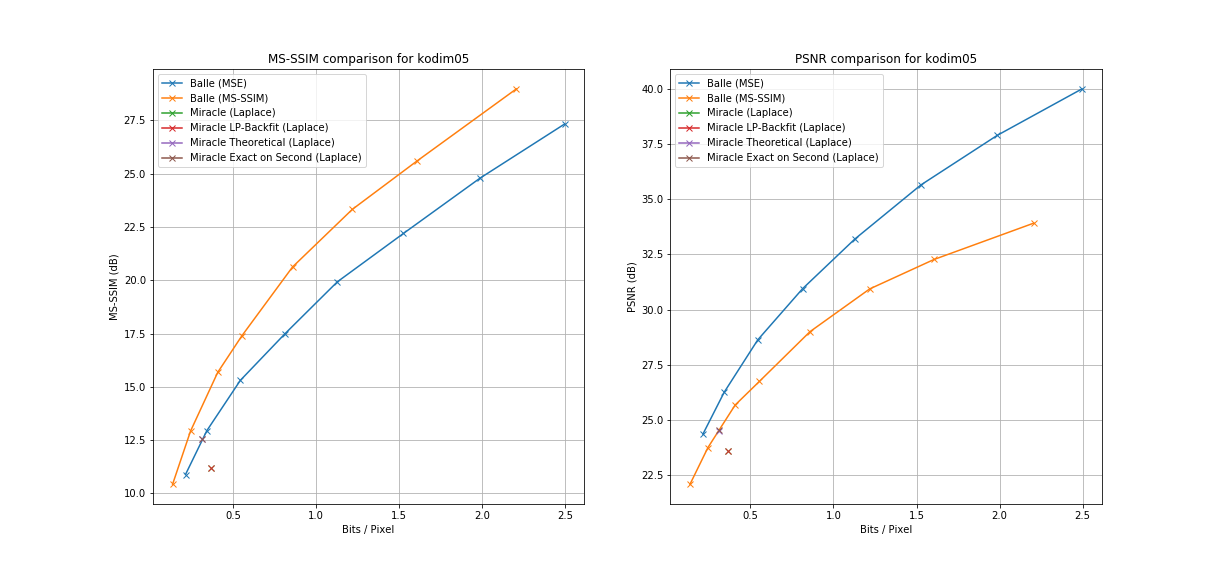
\includegraphics[width=\textwidth]{kodim05_comparison.png}
  \caption[Rate-Distorsion curves of several methods on \texttt{kodim05}]
  {Rate-Distorsion curves of several methods on \texttt{kodim05}. Please see
    Section \ref{sec:experimental_results} for the description of how we
    obtained each curve. MS-SSIM results are presented in
    decibels, where the conversion is done using the formula $-10 \cdot
    \log_{10}\left( 1 - \text{MS-SSIM}(\vec{x}, \hat{\vec{x}}) \right)$.
    PSNR is computed from the mean squared error, using the formula 
    $-10 \cdot \log_{10}\text{MSE}(\vec{x}, \hat{\vec{x}})$.}
  \label{fig:kodim05_comp}
\end{figure}

\par
Somewhat surprisingly, with no fine-tuning, our results, especially the
$\gamma$-PLNs get very close to the state-of-the-art results of
\cite{balle2018variational}. The distrotion gap caused by the greedy method is
clearly exposed: there is an approximately 1-2 dB gap for both PLNs and
$\gamma$-PLNs across all bitrates for both MS-SSIM and PSNR.
The theoretically optimal performance of $\gamma$-PLNs is competitive with the
state-of-the-art on lower bitrates, so finding a better sampling algorithm
is of paramount importance to make our method competitive in general.
\par
On the other hand, we see that the actual bitrates are not much higher than the
theoretically optimal ones, even
though the \textit{actual} numbers include the overheads, such as the list of
group indices for importance sampling.

\par
Interestingly, our methods' curves tail off much more heavily as the bitrate increases,
than other methods. The fact that distortion gap remains the same between the
theoretical and actual curves for both models though indicates that the discrepancy
does not come from the sampling techniques' degrading performance, rather it
must come from the model itself. One contributing factor is the inherent
blurriness of VAE (and by extension PLN) reconstructions with Gaussian latent
distributions. A key indication of this is that the technique of learning
$\gamma$ was introduced by \cite{dai2019diagnosing} with the precise reason of
ameliorating this issue, and indeed our $\gamma$-PLNs do perform significantly
better than the regular ones. Another likely reason is the capacity limitation
of the second level to 24 channels only, although we have not performed
experiments to confirm this due to time constraints. Other possible limitations
might come from a small training dataset size (\cite{balle2018variational} train
on 1,000,000 high resolution images, we train on 585), as well as from the loss
(\cite{balle2018variational} directly optimize a MS-SSIM loss). We leave
investigating all of these reasons to future work.

\paragraph{Contribution of second levels}
An important part of verifying the validity of using PLNs is to analyze the
contribution of the second level. Comparing Figure \ref{fig:vae_rand_posterior}
to Figures \ref{fig:ladder_rand_posterior} and \ref{fig:gamma_rand_posterior},
we saw how using the conditional independence structure instead of the
full independence assumption allows us to model the spatial dependencies between
dimensions far better, which is the clear reason why PLNs heavily outperform VAEs.
As Figure \ref{fig:kodim05_side_info} shows, the second level does not only
greatly improve the distortion, it also does this very efficiently, as we see that
above very low bitrates, it does not contribute more than 10\% of the total bits
per pixel.
\begin{figure}
  \centering
  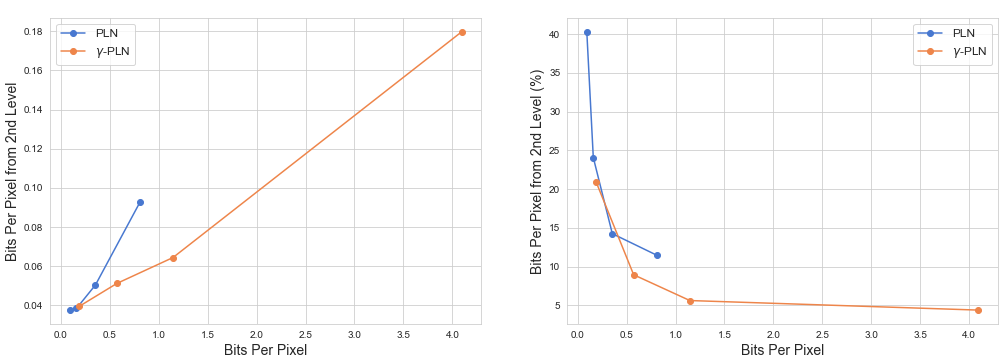
\includegraphics[width=\textwidth]{kodim05_side_info.png}
  \caption[Contribution of the second level to the rate, plotted agains the
    actual rate.]{Contribution of the second level to the rate, plotted agains the
    actual rate. \textbf{Left:} Contribution in BPP, \textbf{Right:}
    Contribution in percentages. We see that for lower bitrates there is more
    contribution from the second level and it quickly decreases for higher
    rates. It is also clear that on the same bitrates, the $\gamma$-PLN requires
    less contribution from the second level than regular PLN.}
  \label{fig:kodim05_side_info}
\end{figure}

\subsection{Compression Speed}
\par
Although not a focus of our project, we now briefly examine the the encoding and
decoding speed of our method. We have plotted the compression ratios of our
models against the time it took them to encode / decode them using IS-GS in
Figure \ref{fig:kodim05_coding_time}. As increasing the reconstruction quality
leads to higher KL divergences between the latent posteriors and priors, both the
importance sampler and the greedy sampler will need to split up a higher total
KL. Thus, we expect the coding to become slower, and is precisely what we
observe, with a seemingly approximately linear growth. We also see that encoding
consistently takes around 3 times as long as decoding. It is clear that our
method is not yet practical:
even the fastest case takes around a minute to encode and about 20 seconds to
decode, which very far away for real-time applications for now. The precise
values are reported in Table \ref{tab:kodim05_coding_time}.
\begin{figure}
  \centering
  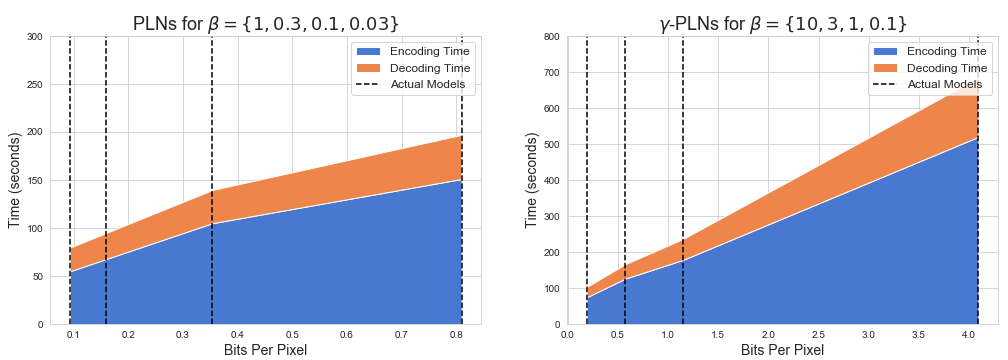
\includegraphics[width=\textwidth]{kodim05_coding_time.png}
  \caption[Coding times of models plotted agains their rates.]
  {Coding times of models plotted agains their rates. \textbf{Left:}
    Regular PLNs. \textbf{Right:} $\gamma$-PLNs. The striped lines indicate
    the concrete positions of our models in the rate line. While it seems
    that there is a
    linear relationship between rate and coding time, we do not have enough
    datapoints to conclude this.}
  \label{fig:kodim05_coding_time}
\end{figure}

\begin{table}[]
  \centering
  \begin{tabular}{|r||c|c|c|c||c|c|c|c|}
    \hline
    & \multicolumn{4}{c||}{\textbf{PLNs}} & \multicolumn{4}{c|}{\textbf{$\gamma$-PLNs}} \\
    \hline 
    $\beta$ & 1 & 0.3 & 0.1 & 0.03 & 10 & 3 & 1 & 0.1 \\ 
    \hline\hline
    Encoding Time (s) & 55.91 & 64.95 & 98.85 & 145.38 & 71.40 & 120.54 & 172.34 & 452.49 \\
    \hline
    Decoding Time (s) & 24.85 & 26.61 & 33.34 & 44.85 & 27.81 & 38.87 & 54.86 & 140.52 \\
    \hline
  \end{tabular}
  \caption{Compression times of our models for various compression rates.}
  \label{tab:kodim05_coding_time}
\end{table}



% ********************************** Back Matter *******************************
% Backmatter should be commented out, if you are using appendices after References
%\backmatter

% ********************************** Bibliography ******************************
\begin{spacing}{0.9}

% To use the conventional natbib style referencing
% Bibliography style previews: http://nodonn.tipido.net/bibstyle.php
% Reference styles: http://sites.stat.psu.edu/~surajit/present/bib.htm

\bibliographystyle{apalike}
%\bibliographystyle{unsrt} % Use for unsorted references  
%\bibliographystyle{plainnat} % use this to have URLs listed in References
\cleardoublepage
\bibliography{References/references} % Path to your References.bib file


% If you would like to use BibLaTeX for your references, pass `custombib' as
% an option in the document class. The location of 'reference.bib' should be
% specified in the preamble.tex file in the custombib section.
% Comment out the lines related to natbib above and uncomment the following line.

%\printbibliography[heading=bibintoc, title={References}]


\end{spacing}

% ********************************** Appendices ********************************

\begin{appendices} % Using appendices environment for more functunality

%!TEX root = ../thesis.tex
% ******************************* Thesis Appendix A ****************************
\chapter{Appendix A} 

\subsection*{Rejection Sampling}
\par
The rejection sampling algorithm presented here is due to
\cite{harsha2007communication}.

\begin{algorithm}
  \caption{Rejection sampling presented in \cite{harsha2007communication}.}
  \label{alg:harsha_rej_sampling}
  \begin{algorithmic}[1]
    \Procedure{Rej-Sampler}{$P, Q, \langle x_i \sim Q \mid i \in \Nats \rangle$}
    \Comment $P$ is the prior
    \Statex
    \Comment $Q$ is the posterior
    \Statex
    \Comment $x_i$ are i.i.d. samples from $Q$
    \State $p_0(x) \gets 0 \quad \forall x \in \X$.
    \State $p_0^* \gets 0$.
    \For{$i \gets 1, \hdots \infty$}

    \State
    $\alpha_i(x) \gets \min{P(x) - p_{i - 1}(x), (1 - p_{i - 1}^*)Q(x)}\quad
    \forall x \in \X$

    \State $p_i(x) \gets p_{i - 1}(x) + \alpha_i(x)$
    
    \State $p_i^* \gets \sum_{x \in \X}p_i(x)$

    \State $\beta_i(x_i) \gets \frac{\alpha_i(x)}{(1 - p_i^*)Q(x)}$

    \State Draw $u \sim \Unif{0, 1}$

    \Statex

    \If{$u < \beta_i(x_i)$}

    \State\Return $i, x_i$

    \EndIf
    
    \EndFor
    \EndProcedure
  \end{algorithmic}
\end{algorithm}

\begin{algorithm}
  \caption{Importance sampling algorithm proposed by \cite{havasi2018minimal}}
  \label{alg:miracle_imp_samp}
  \begin{algorithmic}
    \Procedure{Importance-Sampler}{$P, Q, \langle x_i \sim Q \mid i \in \Nats \rangle$}
    \Comment $P$ is the prior
    \Statex
    \Comment $Q$ is the posterior
    \Statex
    \Comment $x_i$ are i.i.d. samples from $Q$

    \State $K \gets \exp\{\KL{Q}{P}\}$

    \State $\tilde{w}_i \gets \frac{Q(x_i)}{P(x_i)} \quad \forall i =
    1,\hdots K$

    \State Sample $j \sim p(\tilde{w})$

    \Return $j, x_j$
    \Statex
    \EndProcedure
  \end{algorithmic}
\end{algorithm}

%!TEX root = ../thesis.tex
% ******************************* Thesis Appendix B ********************************

\chapter{Further Image Comparisons}
\label{chapter:appendix_b}

\graphicspath{{../img/plots/kodak_comparison/}{../img/plots/kodak_coding_time/}{../img/plots/kodak_side_info/}{../img/plots/reconstructions/}}


\par In this appendix we present some further reconstruction comparisons for the
models we trained. All of the plots presented in this appendix as well as plots
for images are available online at
\url{https://github.com/gergely-flamich/miracle-compression/tree/master/img/plots}. 

\paragraph{}
The images and their statistics are displayed in the following order:
\texttt{kodim04}, \texttt{kodim10} and \texttt{kodim17}.
For each image, we first present their regular PLN and then their $\gamma$-PLN
reconstructions.
The $\beta$s corresponding to the images in the quartered comparison plots are
shown in Table \ref{tab:beta_layout}.
We also present the compression comparison plot and the side information plot
as described in Chapter \ref{chapter:experiments}.
\begin{table}[H]
  \centering
  \begin{tabular}{|r|c|c|c|c|}
    \hline
    & \textbf{Top Left} & \textbf{Top Right} & \textbf{Bottom Left} & \textbf{Bottom Right} \\
    \hline\hline
    Regular PLNs & 0.03 & 0.1 & 0.3 & 1 \\
    \hline
    $\gamma$-PLNs & 0.1 & 1 & 3 & 10 \\
    \hline
  \end{tabular}
  \caption{$\beta$s used in the quartered comparison plots for PLNs and $\gamma$-PLNs.}
  \label{tab:beta_layout}
\end{table}


% ======================================================================
% Kodak 04
% ======================================================================
\begin{figure}
  \centering
  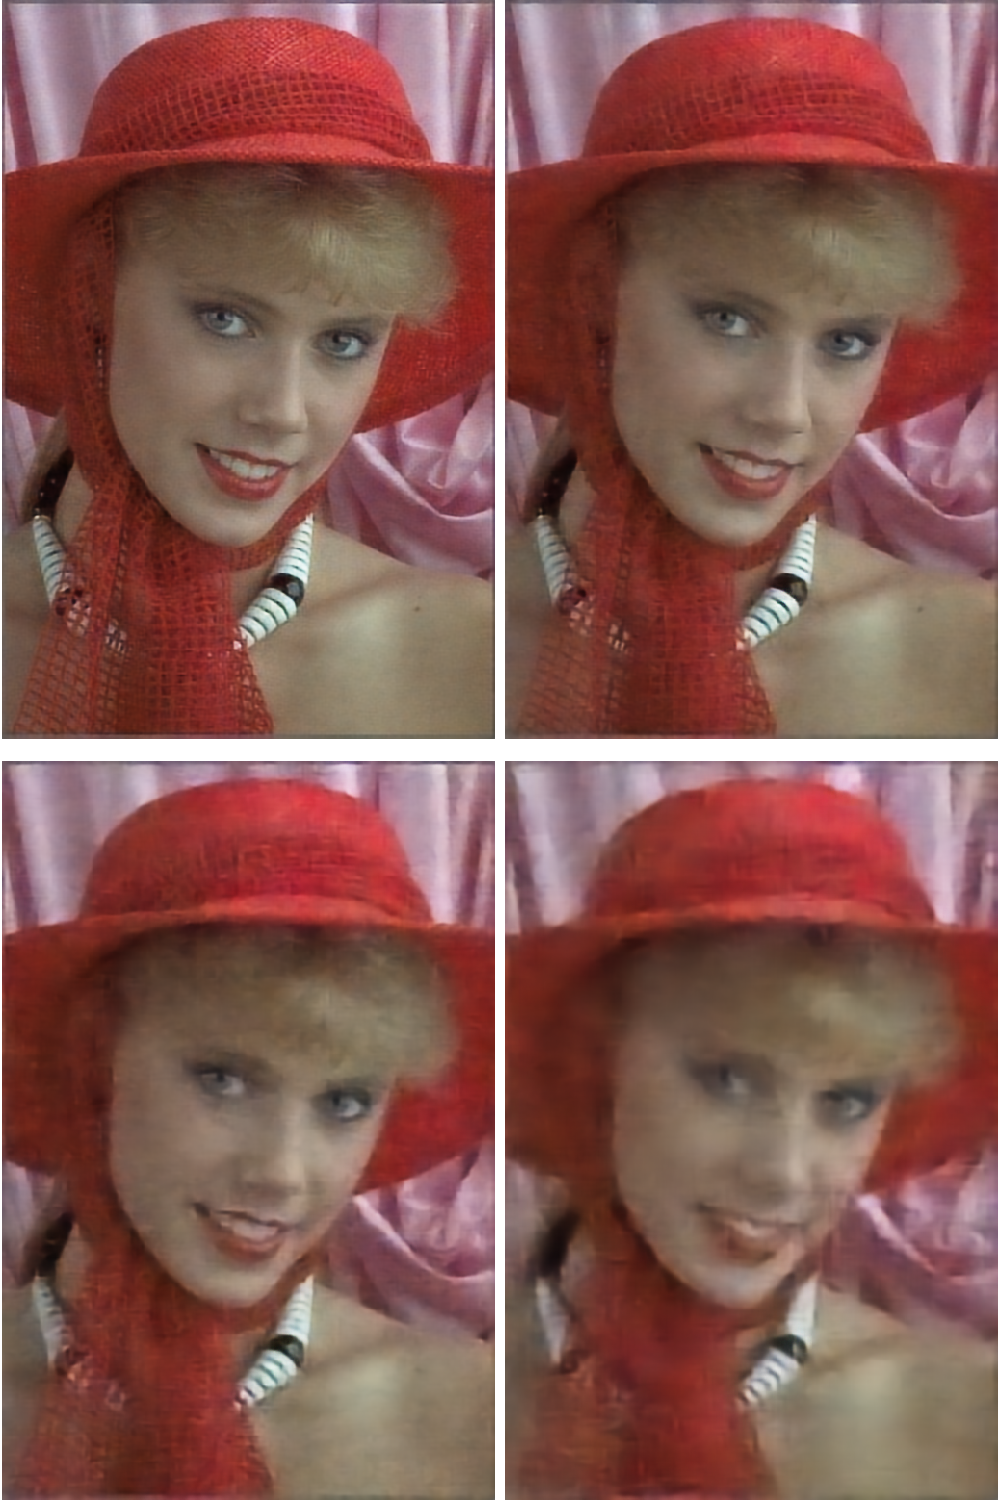
\includegraphics[width=\textwidth]{pln_003_01_03_1_k04.png}
\end{figure}
\begin{figure}
  \centering
  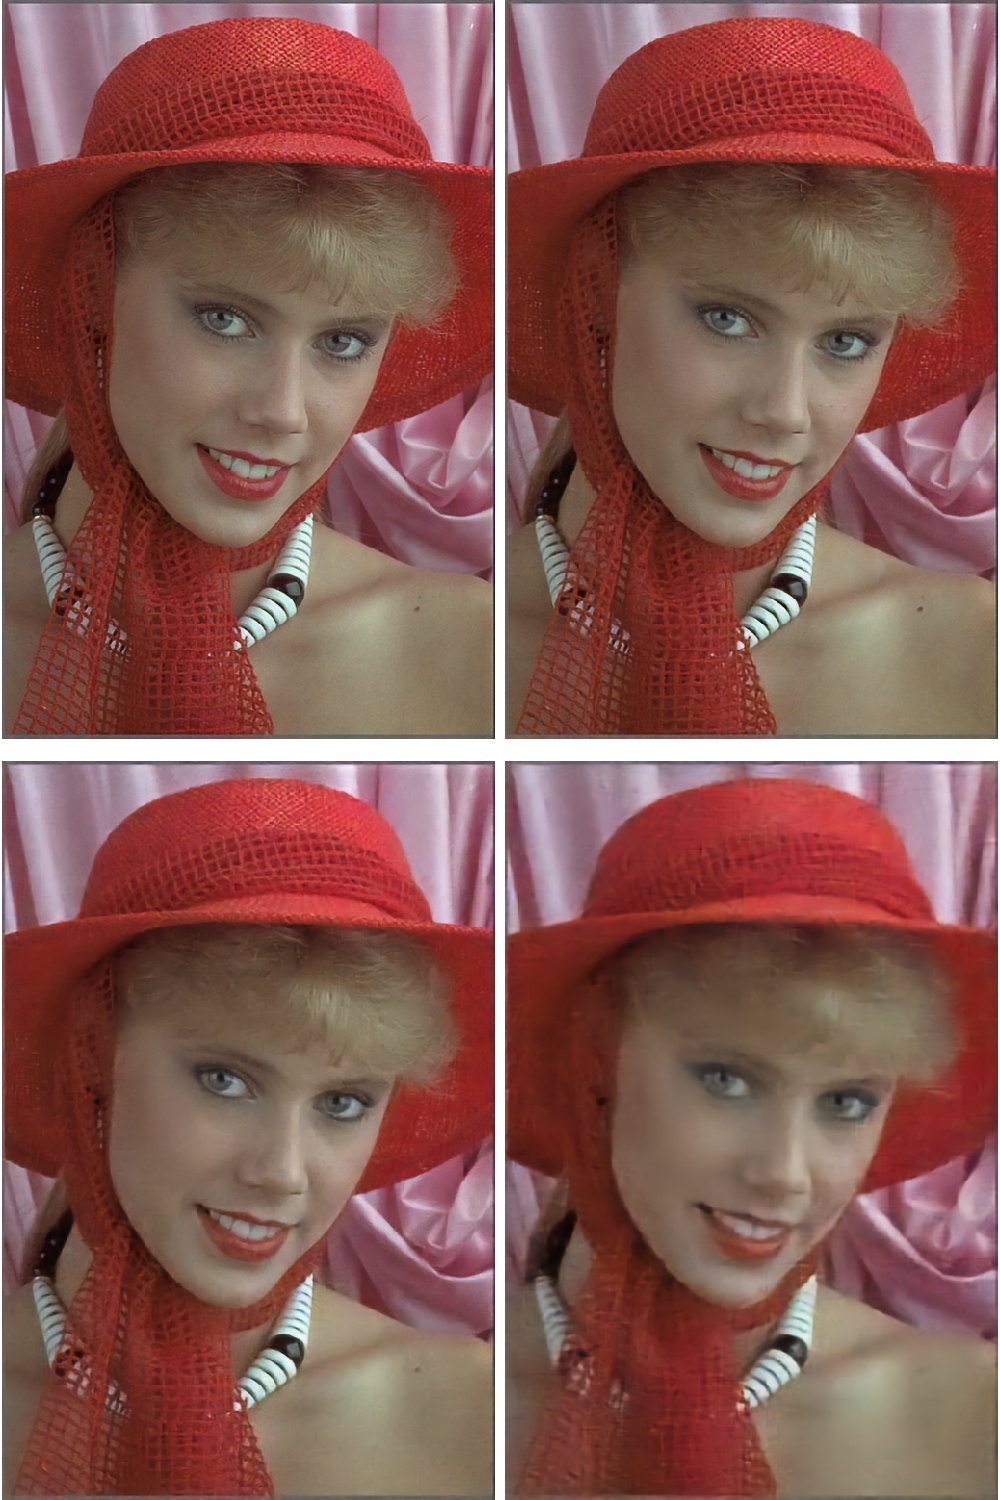
\includegraphics[width=\textwidth]{log_gamma_01_1_3_10_k04.png}
\end{figure}
\begin{figure}
  \centering
  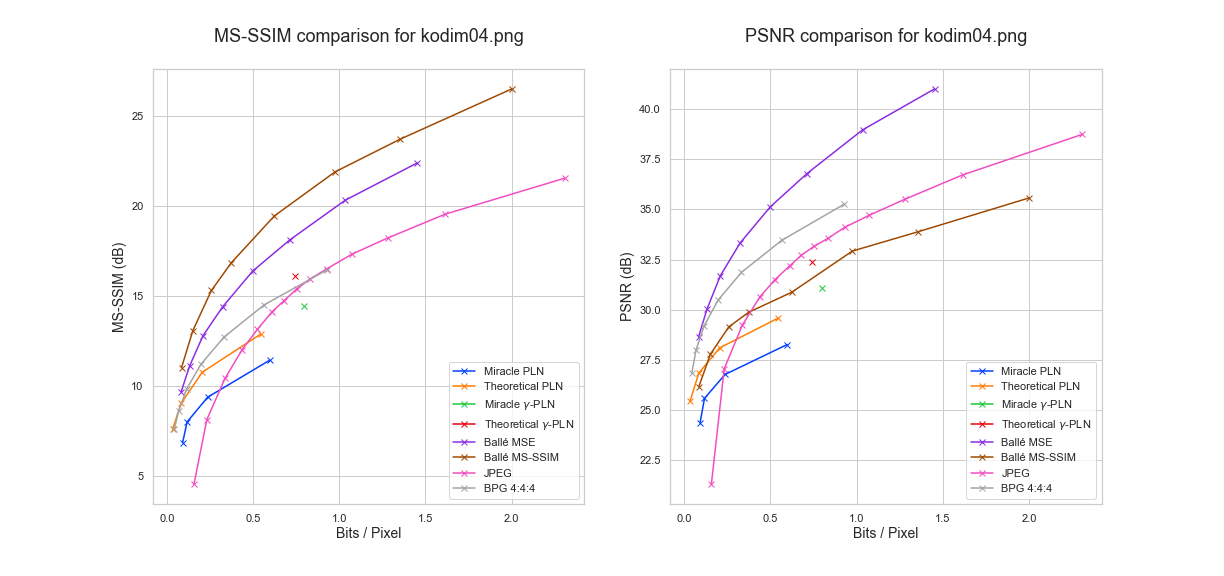
\includegraphics[width=\textwidth]{kodim04_comparison.png}
\end{figure}
\begin{figure}
  \centering
  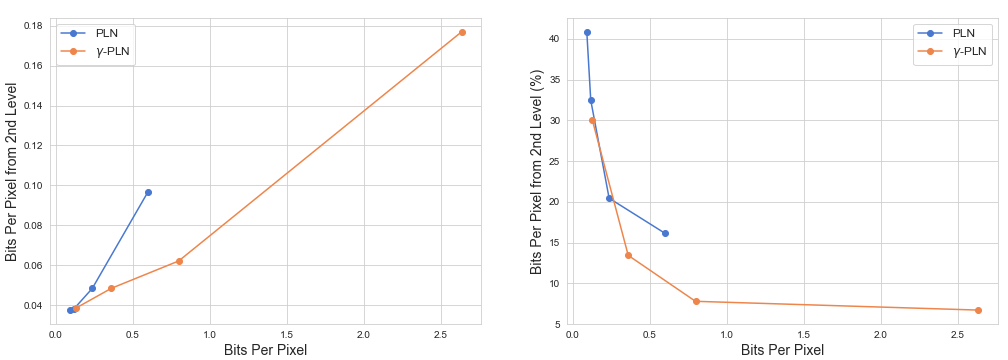
\includegraphics[width=\textwidth]{kodim04_side_info.png}
\end{figure}

% ======================================================================
% Kodak 10
% ======================================================================
\begin{figure}
  \centering
  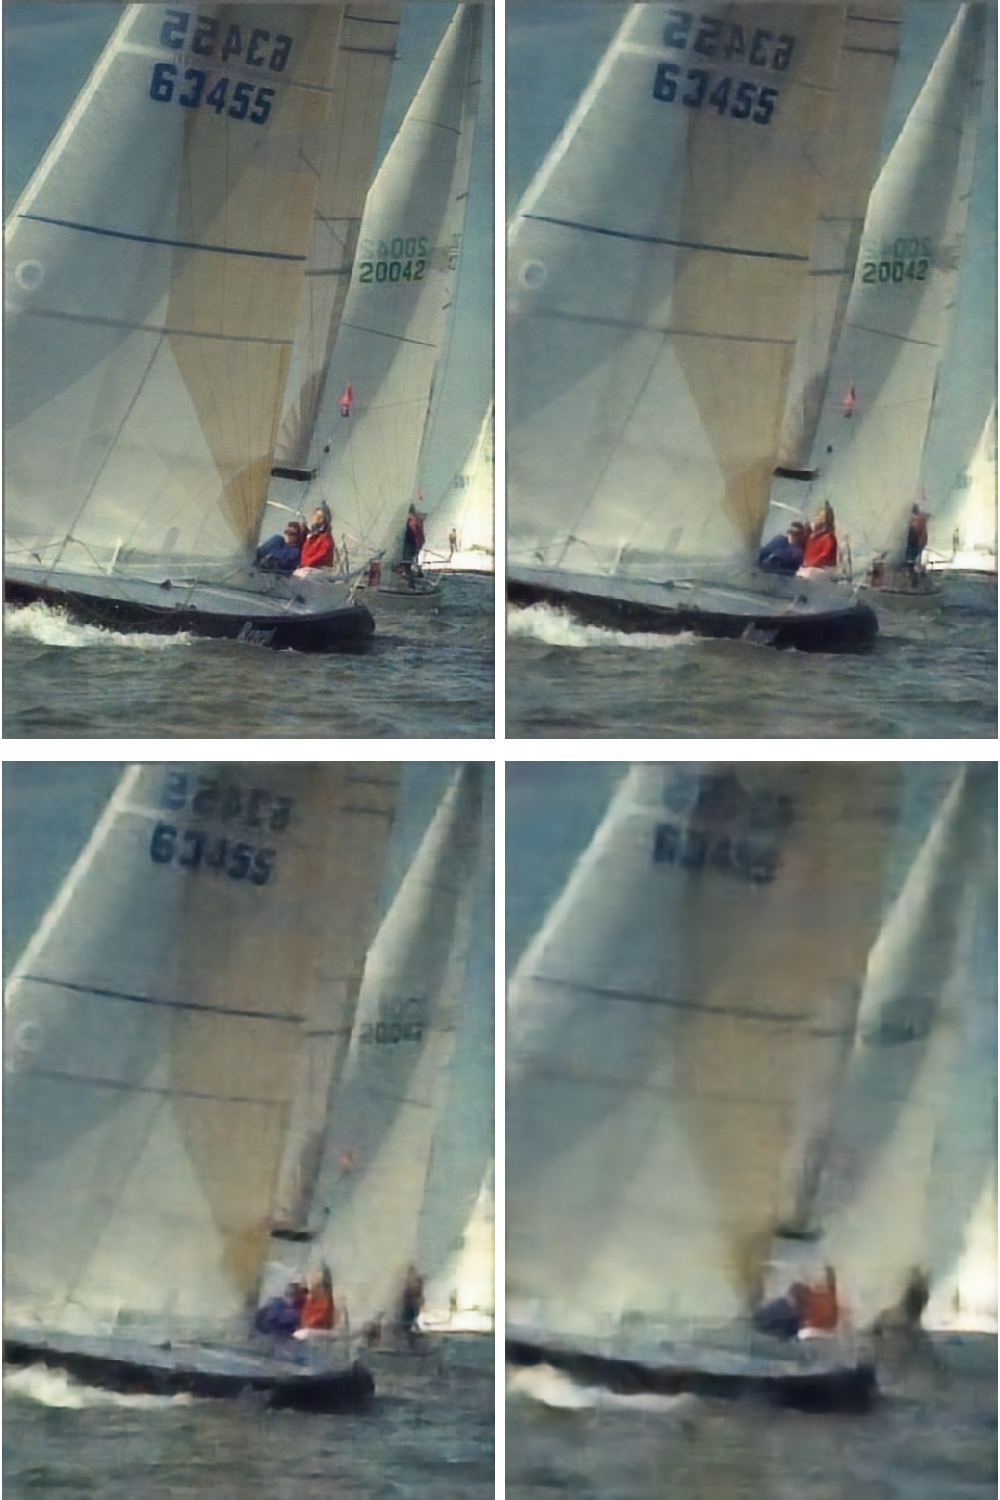
\includegraphics[width=\textwidth]{pln_003_01_03_1_k10.png}
\end{figure}
\begin{figure}
  \centering
  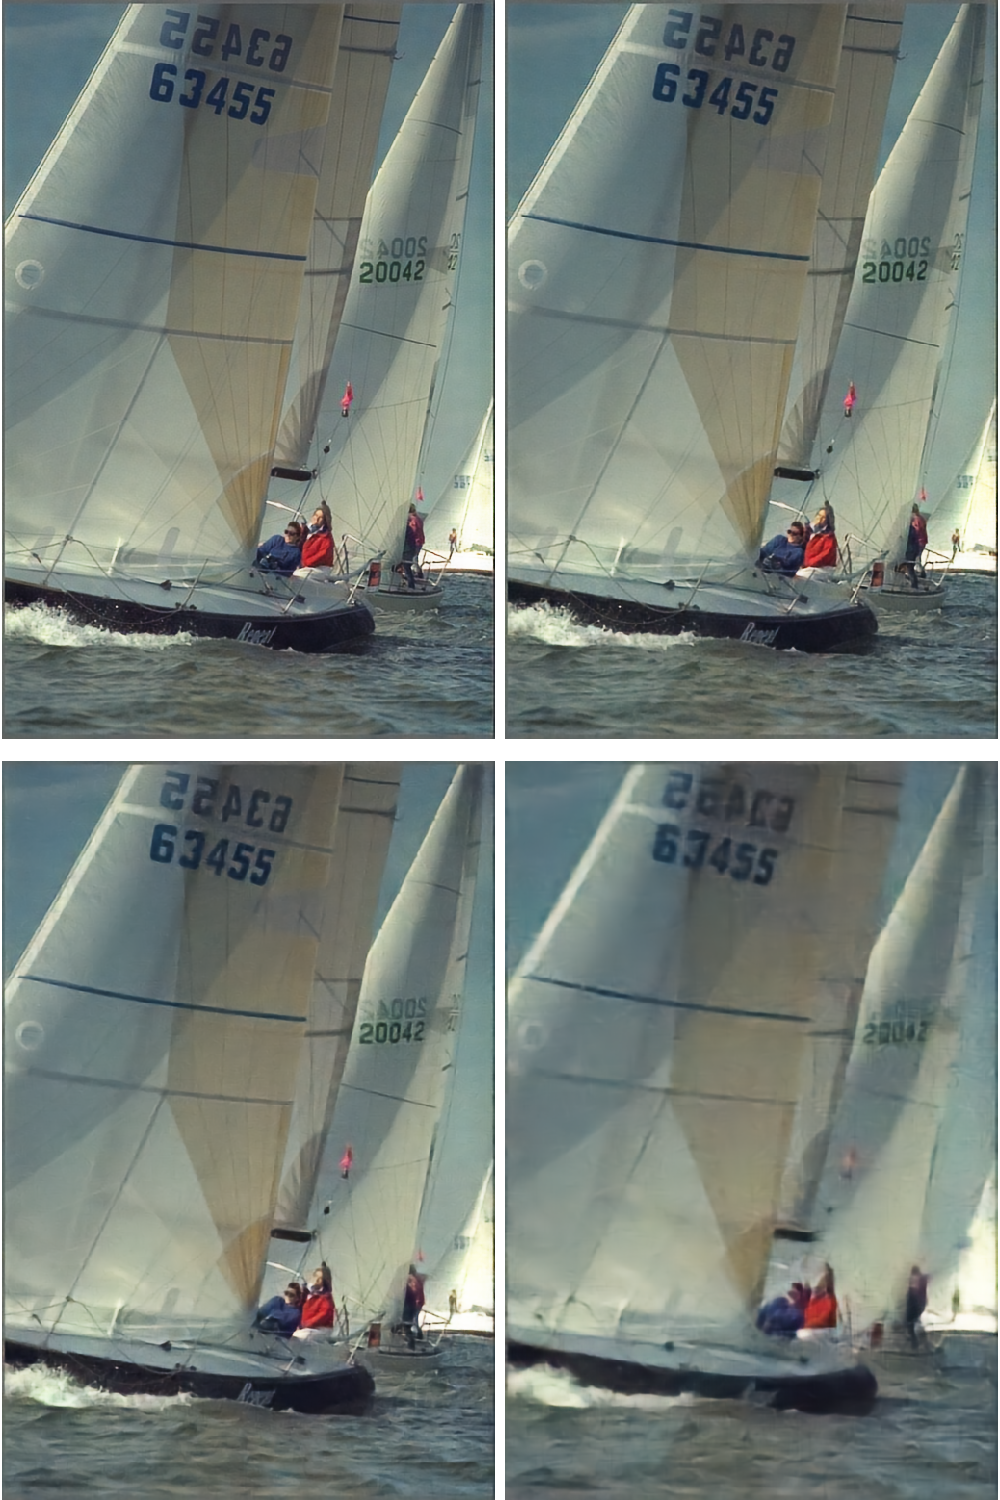
\includegraphics[width=\textwidth]{log_gamma_01_1_3_10_k10.png}
\end{figure}
\begin{figure}
  \centering
  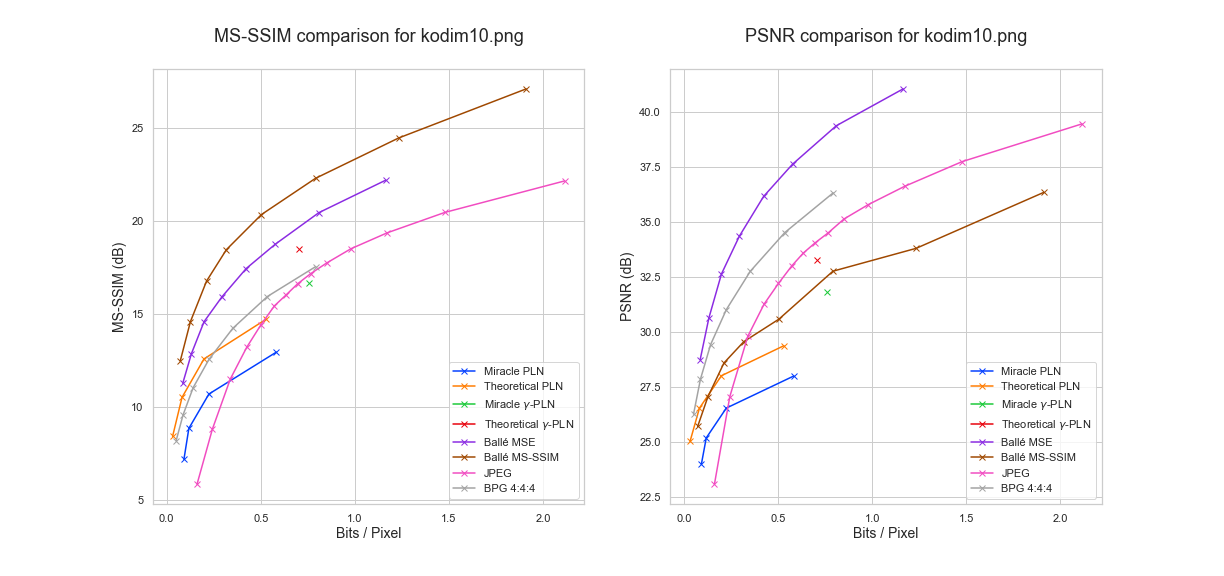
\includegraphics[width=\textwidth]{kodim10_comparison.png}
\end{figure}
\begin{figure}
  \centering
  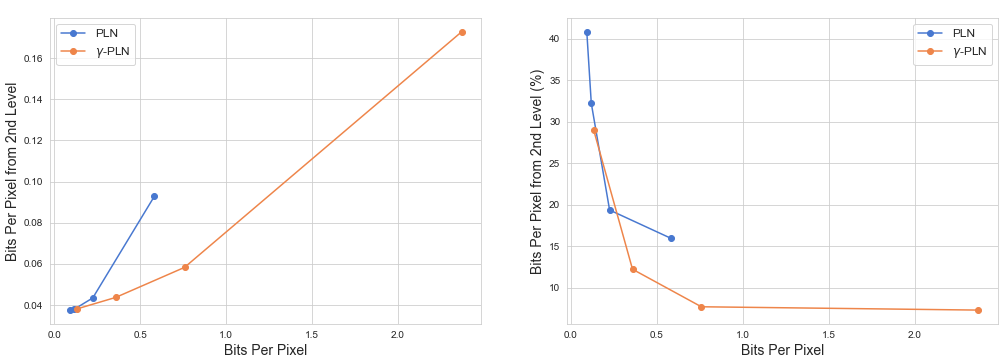
\includegraphics[width=\textwidth]{kodim10_side_info.png}
\end{figure}

% ======================================================================
% Kodak 17
% ======================================================================
\begin{figure}
  \centering
  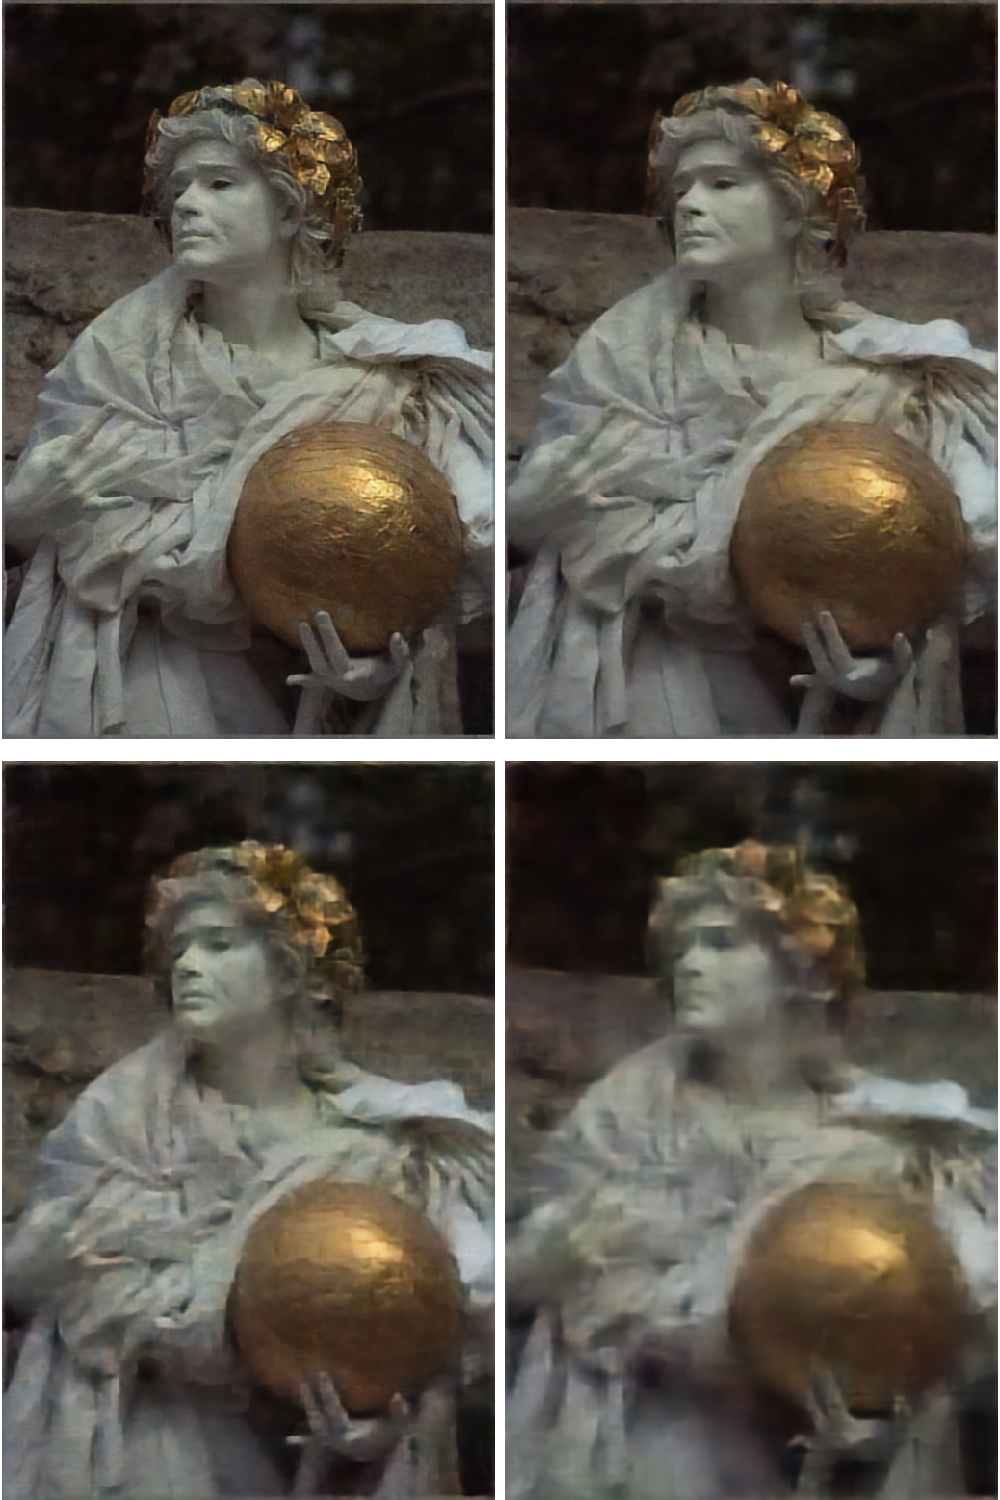
\includegraphics[width=\textwidth]{pln_003_01_03_1_k17.png}
\end{figure}
\begin{figure}
  \centering
  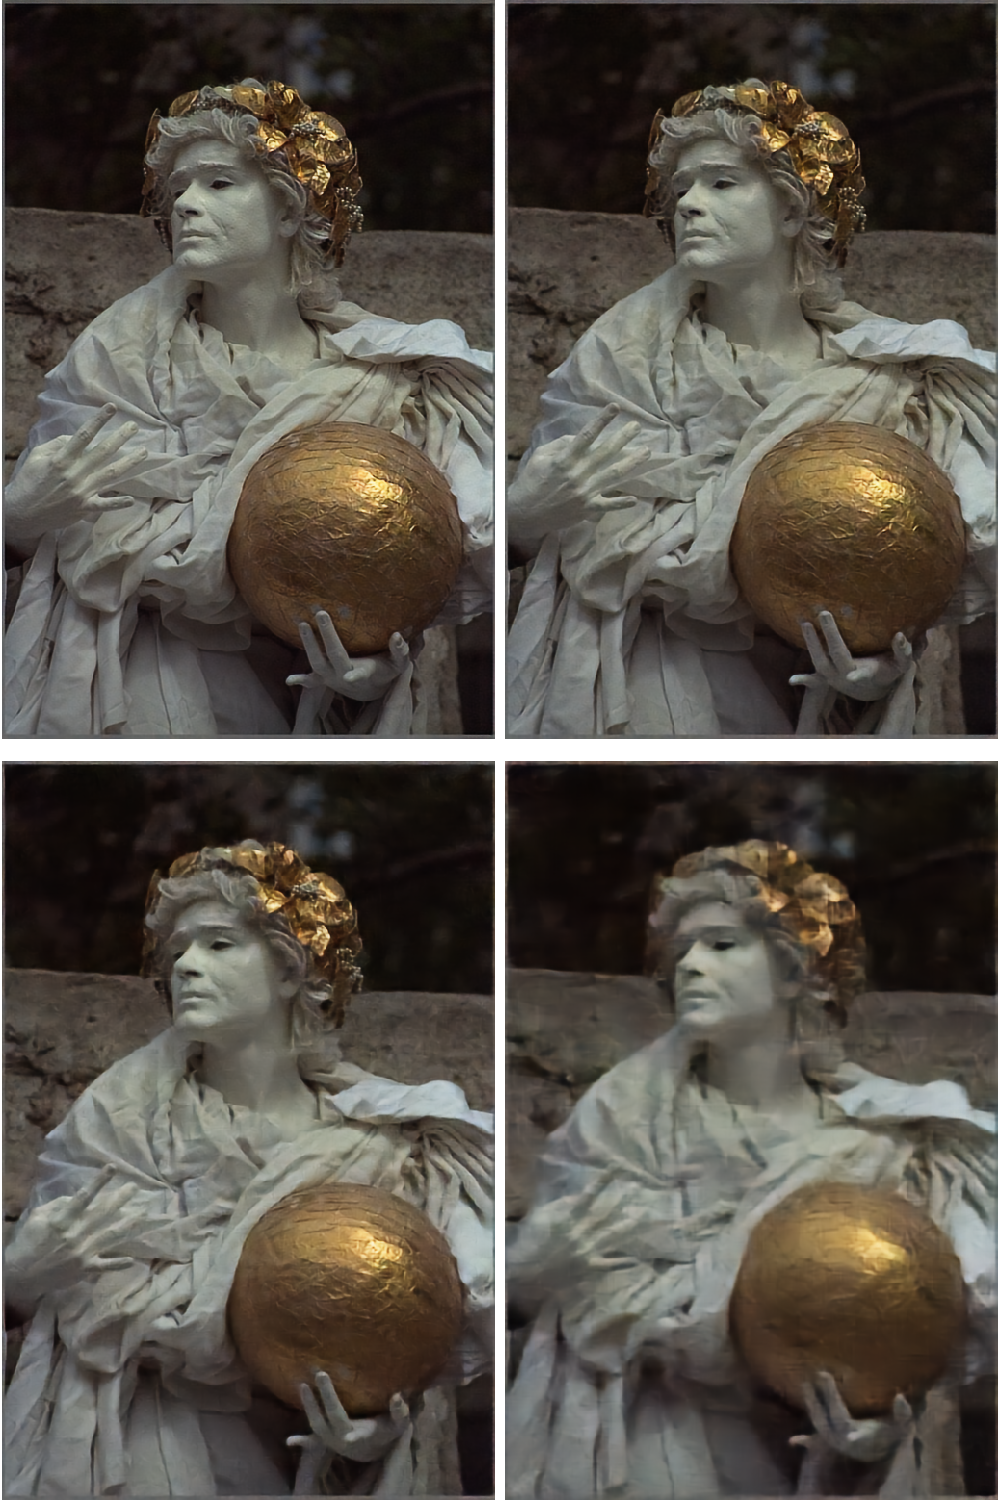
\includegraphics[width=\textwidth]{log_gamma_01_1_3_10_k17.png}
\end{figure}
\begin{figure}
  \centering
  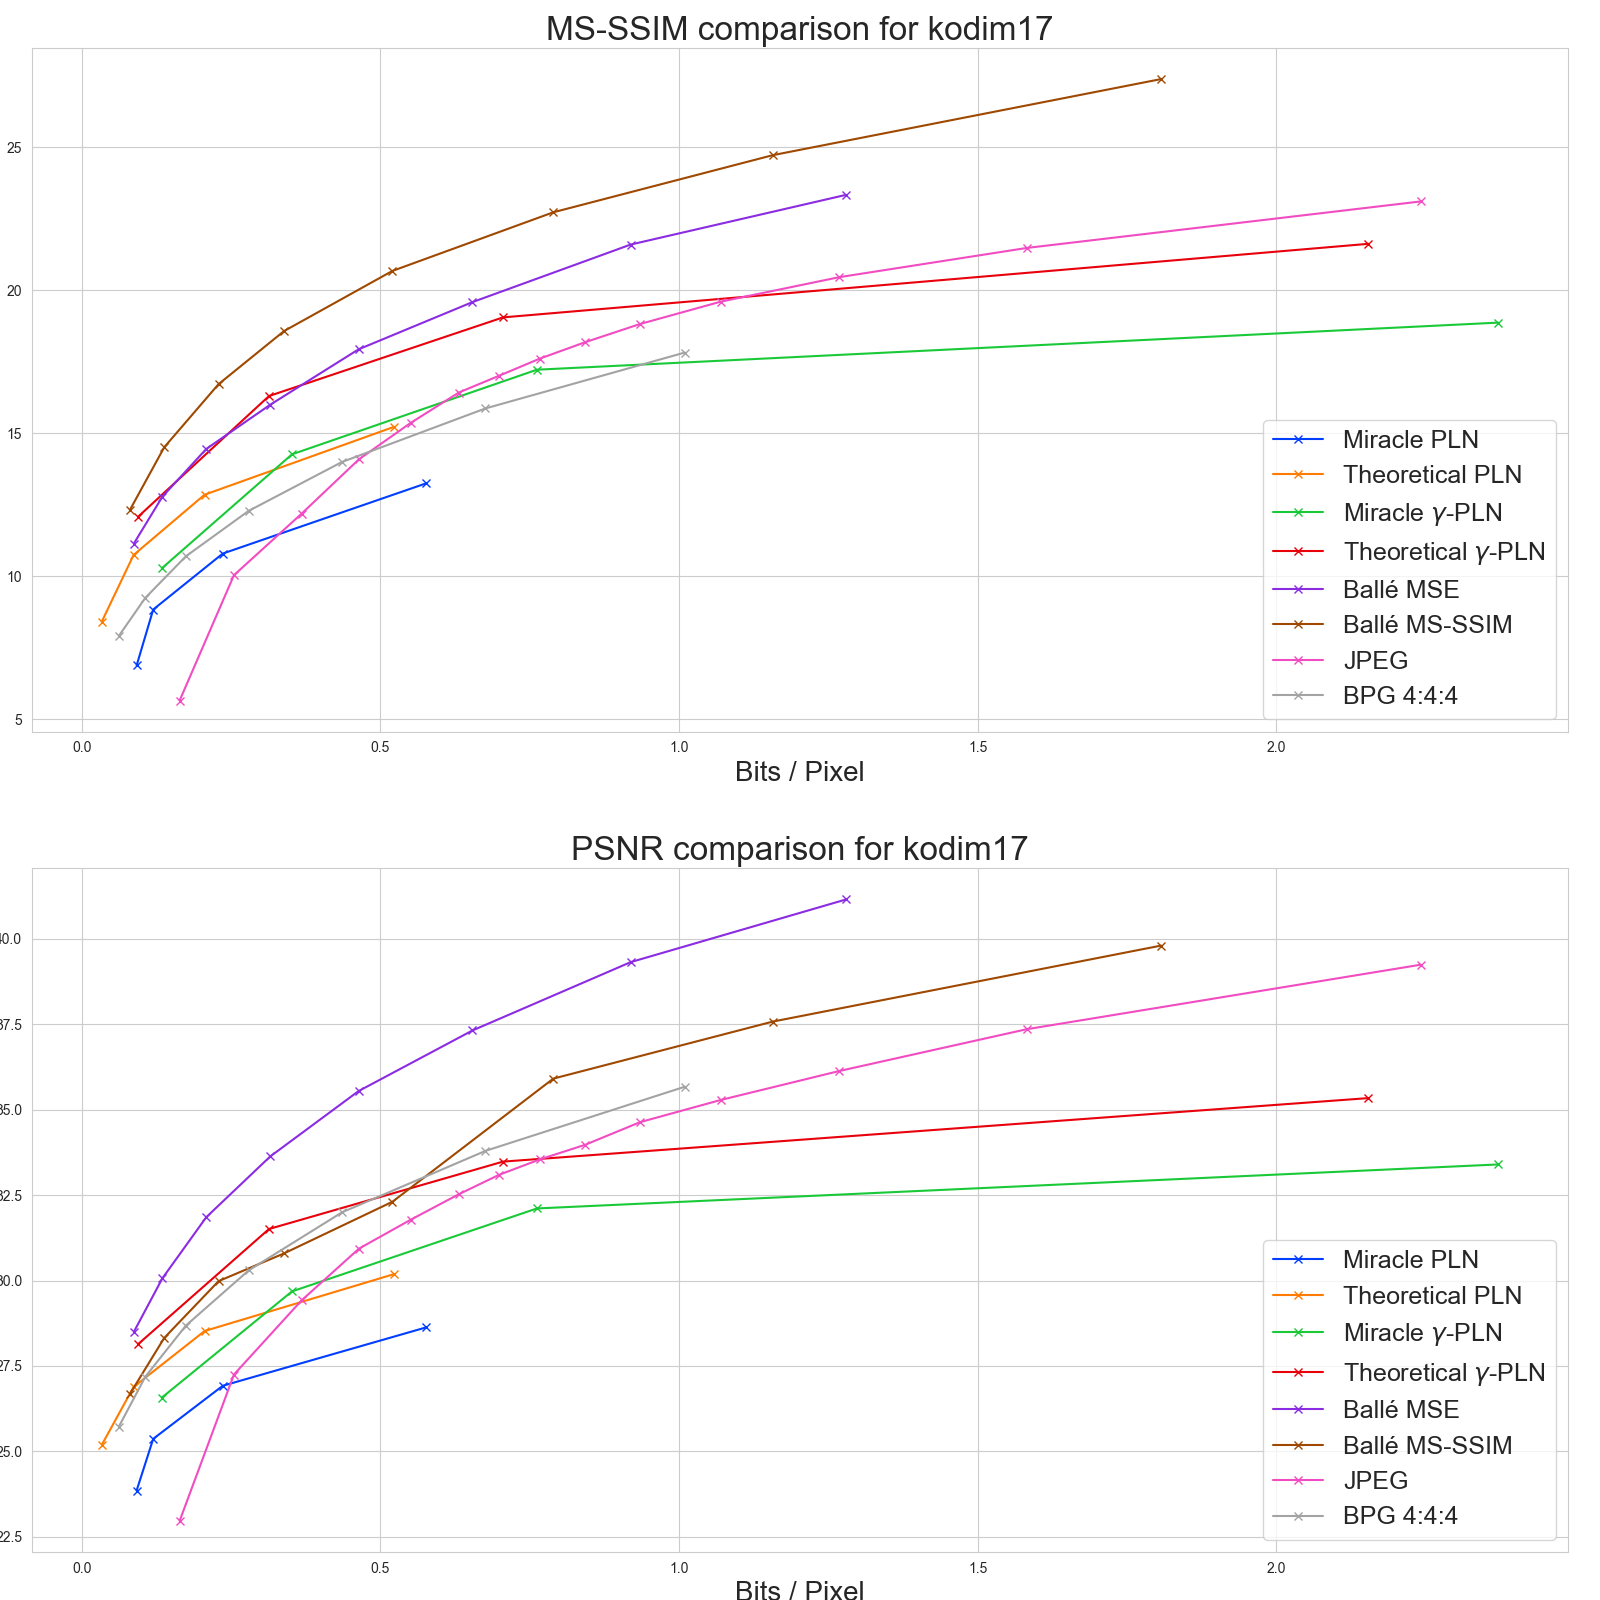
\includegraphics[width=\textwidth]{kodim17_comparison.png}
\end{figure}
\begin{figure}
  \centering
  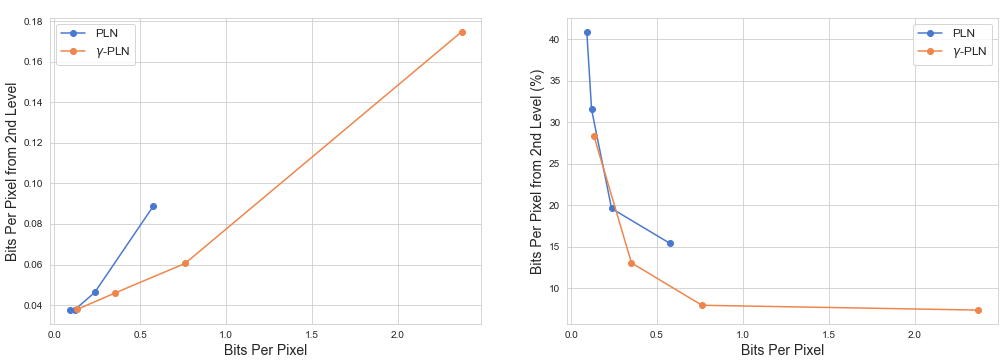
\includegraphics[width=\textwidth]{kodim17_side_info.png}
\end{figure}

\end{appendices}

% *************************************** Index ********************************
\printthesisindex % If index is present

\end{document}
